% Options for packages loaded elsewhere
\PassOptionsToPackage{unicode}{hyperref}
\PassOptionsToPackage{hyphens}{url}
%
\documentclass[
]{article}
\usepackage{amsmath,amssymb}
\usepackage{lmodern}
\usepackage{ifxetex,ifluatex}
\ifnum 0\ifxetex 1\fi\ifluatex 1\fi=0 % if pdftex
  \usepackage[T1]{fontenc}
  \usepackage[utf8]{inputenc}
  \usepackage{textcomp} % provide euro and other symbols
\else % if luatex or xetex
  \usepackage{unicode-math}
  \defaultfontfeatures{Scale=MatchLowercase}
  \defaultfontfeatures[\rmfamily]{Ligatures=TeX,Scale=1}
\fi
% Use upquote if available, for straight quotes in verbatim environments
\IfFileExists{upquote.sty}{\usepackage{upquote}}{}
\IfFileExists{microtype.sty}{% use microtype if available
  \usepackage[]{microtype}
  \UseMicrotypeSet[protrusion]{basicmath} % disable protrusion for tt fonts
}{}
\makeatletter
\@ifundefined{KOMAClassName}{% if non-KOMA class
  \IfFileExists{parskip.sty}{%
    \usepackage{parskip}
  }{% else
    \setlength{\parindent}{0pt}
    \setlength{\parskip}{6pt plus 2pt minus 1pt}}
}{% if KOMA class
  \KOMAoptions{parskip=half}}
\makeatother
\usepackage{xcolor}
\IfFileExists{xurl.sty}{\usepackage{xurl}}{} % add URL line breaks if available
\IfFileExists{bookmark.sty}{\usepackage{bookmark}}{\usepackage{hyperref}}
\hypersetup{
  pdftitle={Supplement for: Carbon cycling in mature and regrowth forests globally},
  hidelinks,
  pdfcreator={LaTeX via pandoc}}
\urlstyle{same} % disable monospaced font for URLs
\usepackage[margin=1in]{geometry}
\usepackage{graphicx}
\makeatletter
\def\maxwidth{\ifdim\Gin@nat@width>\linewidth\linewidth\else\Gin@nat@width\fi}
\def\maxheight{\ifdim\Gin@nat@height>\textheight\textheight\else\Gin@nat@height\fi}
\makeatother
% Scale images if necessary, so that they will not overflow the page
% margins by default, and it is still possible to overwrite the defaults
% using explicit options in \includegraphics[width, height, ...]{}
\setkeys{Gin}{width=\maxwidth,height=\maxheight,keepaspectratio}
% Set default figure placement to htbp
\makeatletter
\def\fps@figure{htbp}
\makeatother
\setlength{\emergencystretch}{3em} % prevent overfull lines
\providecommand{\tightlist}{%
  \setlength{\itemsep}{0pt}\setlength{\parskip}{0pt}}
\setcounter{secnumdepth}{-\maxdimen} % remove section numbering
\usepackage{float} \usepackage{caption} \captionsetup[table]{font=footnotesize} \captionsetup[figure]{font=footnotesize} \captionsetup[figure]{labelformat=empty} \captionsetup[table]{labelformat=empty} \usepackage{pdflscape} \newcommand{\blandscape}{\begin{landscape}} \newcommand{\elandscape}{\end{landscape}}
\usepackage{setspace}\onehalfspacing
\usepackage{booktabs}
\usepackage{longtable}
\usepackage{array}
\usepackage{multirow}
\usepackage{wrapfig}
\usepackage{float}
\usepackage{colortbl}
\usepackage{pdflscape}
\usepackage{tabu}
\usepackage{threeparttable}
\usepackage{threeparttablex}
\usepackage[normalem]{ulem}
\usepackage{makecell}
\usepackage{xcolor}
\ifluatex
  \usepackage{selnolig}  % disable illegal ligatures
\fi

\title{Supplement for: Carbon cycling in mature and regrowth forests
globally}
\author{}
\date{\vspace{-2.5em}}

\begin{document}
\maketitle

{
\setcounter{tocdepth}{2}
\tableofcontents
}
\raggedright

\newpage

\hypertarget{appendix-s1.-duplicates-and-conflicting-records-within-forc}{%
\subsection{Appendix S1. Duplicates and Conflicting Records within
ForC}\label{appendix-s1.-duplicates-and-conflicting-records-within-forc}}

\hypertarget{status-of-duplicates-and-conflicting-records-within-forc}{%
\subsubsection{Status of duplicates and conflicting records within
ForC}\label{status-of-duplicates-and-conflicting-records-within-forc}}

\emph{ForC} v3.0 contains potential duplicates that have arisen from
importing intermediary data sets with overlap in data. In particular,
the recent imports of \emph{SRDB} and \emph{GROA} resulted in the
introduction of numerous potential duplicates. \emph{SRDB} and
\emph{ForC} were developed independently (but with different foci),
resulting in numerous duplicates. The \emph{GROA} database was developed
semi-independently, incorporating \emph{ForC} data partway through its
development. For records retaining the same site names, \emph{GROA}
duplicates were not imported into \emph{ForC} (although they were
checked against corresponding \emph{ForC} records, and differences
reconciled). There were, however, some records entered into \emph{GROA}
independently of \emph{ForC}, resulting in mismatched names.

Prior to the merging of the three databases (\emph{ForC} v2.0,
\emph{SRDB}, and \emph{GROA}), there were potential duplicates within
the \emph{ForC} and \emph{SRDB} portions, the latter an artifact of how
data were recorded in \emph{SRDB} and imported into \emph{ForC.}
\emph{GROA} has no known duplicates, with several steps having been
taken to ensure independence of the records within the database.

To the extent possible, we used automated scripts in R to detect and
remove duplicate records in the creation of \emph{ForC-simplified}.

\hypertarget{handling-within-plot-duplicates}{%
\subsubsection{Handling within-plot
duplicates}\label{handling-within-plot-duplicates}}

Duplicate records within a plot and taken in the same year were
reconciled as follows. Replicate measurements (\emph{i.e.}, replicates
from within a single study) were averaged. Records that subsumed
others---- \emph{i.e.}, the time period included that of \(\ge\) 2 other
records or dates were unknown and therefore conflicted with \(\ge\) 2
other records---were removed. For each group of duplicate
records---\emph{i.e.}, measurements of the same variable in the same
plot at the same time---one record was assigned precedence as follows.
If duplicates were exact matches, one was dropped. When measurement
periods overlapped or were not specified, precedence was given first to
records representing longer measurement periods (\emph{i.e.}, multi-year
mean over a single year) and then to more recently published values. We
manually reviewed duplicates that differed only in methodology,
assigning precedence to the record employing a more comprehensive
approach (\emph{e.g.}, inclusion of understory, lianas, or bamboo as
opposed to just trees) or using a favored methodology.

\hypertarget{handling-duplicate-sites}{%
\subsubsection{Handling duplicate
sites}\label{handling-duplicate-sites}}

To handle cases where duplicate records had different site and/or plot
names (and often slightly different geographic coordinates), we detected
potential duplicates and, for those that had not yet been resolved,
included only one in \emph{ForC-simplified} and the analyses that were
based on it. Potential duplicates were defined as records for the same
variable made in the same year (when known) on stands of similar age and
in the same geographic area (see Methods). Because records of stand age
often lack precision and were sometimes recorded differently in
different intermediary databases, we considered records to be potential
duplicates when ages fell within one of several broad age groups:
\textless10, 10-50, 50-100, and \textgreater100 years (or mature and of
undefined age). We then generated groups of potential duplicates grouped
by variable, geographic area, stand age grouping, and measurement year.

Within each group, we flagged records as potential duplicates--and
excluded them from \emph{ForC-simplified} until they can be
reconciled--as follows. Because \emph{GROA} is believed to contain no
duplicates, all records originating from \emph{GROA} were assumed
independent, and any other records within the group flagged as potential
duplicates. If all records originated from \emph{ForC v2.0} or
\emph{SRDB}, we gave precedence to \emph{ForC} records, flagging
\emph{SRDB} records as potential duplicates. If duplicates remained
(within \emph{ForC v2.0} or \emph{SRDB}), we selected a record for
retention based on citation year, keeping the oldest (presumably
original) citations for most variables. For eddy-covariance variables
(\(NEP\), \(GPP\), \(R_{eco}\)), we retained the record associated with
the most recent publication (most often FLUXNET2015), as these data are
commonly re-assessed using new analysis methods. If publication years
were the same, we randomly selected one record.

This approach was conservative in that it removed some legitimately
independent records. Future refinement of this process and manual review
of potential duplicates will be needed to include
legitimately-independent records in ForC-simplified and in analyses.

\newpage

\hypertarget{table-s1.-numbers-of-records-by-biome-and-age-class}{%
\subsection{Table S1. Numbers of records by biome and age
class}\label{table-s1.-numbers-of-records-by-biome-and-age-class}}

\begin{table}
\centering\begingroup\fontsize{10}{12}\selectfont

\begin{tabular}{lrr}
\toprule
\multicolumn{1}{c}{ } & \multicolumn{2}{c}{n records} \\
\cmidrule(l{3pt}r{3pt}){2-3}
Biome & Mature & Young\\
\midrule
\addlinespace[1em]
\multicolumn{3}{l}{\textbf{Boreal climate zones}}\\
\hspace{1em}Boreal broadleaf & 3 & 326\\
\textbf{\hspace{1em}Boreal conifer} & \textbf{491} & \textbf{919}\\
\hspace{1em}Boreal Other & 46 & 151\\
\addlinespace[1em]
\multicolumn{3}{l}{\textbf{Excluded climate zones}}\\
\hspace{1em}Other broadleaf & 6 & 111\\
\hspace{1em}Other conifer & 30 & 45\\
\hspace{1em}Other Other & 6 & 29\\
\addlinespace[1em]
\multicolumn{3}{l}{\textbf{Temperate climate zones}}\\
\textbf{\hspace{1em}Temperate broadleaf} & \textbf{650} & \textbf{3159}\\
\textbf{\hspace{1em}Temperate conifer} & \textbf{563} & \textbf{2730}\\
\hspace{1em}Temperate Other & 159 & 2363\\
\addlinespace[1em]
\multicolumn{3}{l}{\textbf{Tropical climate zones}}\\
\textbf{\hspace{1em}Tropical broadleaf} & \textbf{835} & \textbf{2576}\\
\hspace{1em}Tropical conifer & 3 & 1\\
\hspace{1em}Tropical Other & 8 & 0\\
\bottomrule
\end{tabular}
\endgroup{}
\end{table}

Sample sizes refer to data set after merging of duplicates, removal of
stands with no age or history data, and removal of managed and disturbed
stands. For vegetation type, ``Other'' refers to stands that are mixed
broadleaf/ conifer or that have not been classified. Focal biomes are
indicated in bold.

\newpage

\hypertarget{table-s2.-model-parameter-estimates-for-age-trends-and-biome-differences-in-young-forests}{%
\subsection{Table S2. Model parameter estimates for age trends and biome
differences in young
forests}\label{table-s2.-model-parameter-estimates-for-age-trends-and-biome-differences-in-young-forests}}

\begingroup\fontsize{7}{9}\selectfont

\begin{longtable}{lllll}
\toprule
Variable & Parameter & Estimate & SE & $t_{value}$\\
\midrule
\endfirsthead
\multicolumn{5}{@{}l}{\textit{(continued)}}\\
\toprule
Variable & Parameter & Estimate & SE & $t_{value}$\\
\midrule
\endhead

\endfoot
\bottomrule
\endlastfoot
\addlinespace[1em]
\multicolumn{4}{l}{\textbf{}}\\
\hspace{1em}$NEP$ & log10(stand.age) & 0.58 & 0.76 & 0.77\\
\hspace{1em} & BiomeTemperate broadleaf & 1.33 & 1.26 & 1.05\\
\hspace{1em} & BiomeTemperate conifer & -2.52 & 0.7 & -3.59\\
\hspace{1em} & BiomeBoreal conifer & 0.2 & 1.05 & 0.19\\
\hspace{1em} & log10(stand.age):BiomeTemperate conifer & 3.35 & 0.88 & 3.83\\
\hspace{1em} & log10(stand.age):BiomeBoreal conifer & -0.16 & 0.97 & -0.16\\
\addlinespace[1em]
\multicolumn{4}{l}{\textbf{}}\\
\hspace{1em}$GPP$ & log10(stand.age) & 1.99 & 2.31 & 0.86\\
\hspace{1em} & BiomeTemperate broadleaf & 11.76 & 3.86 & 3.05\\
\hspace{1em} & BiomeTemperate conifer & 11.15 & 2.08 & 5.35\\
\hspace{1em} & BiomeBoreal conifer & 5.23 & 3.96 & 1.32\\
\hspace{1em} & log10(stand.age):BiomeTemperate conifer & 1.44 & 2.69 & 0.54\\
\hspace{1em} & log10(stand.age):BiomeBoreal conifer & 0.13 & 3.31 & 0.04\\
\addlinespace[1em]
\multicolumn{4}{l}{\textbf{}}\\
\hspace{1em}$NPP$ & log10(stand.age) & -0.27 & 0.68 & -0.4\\
\hspace{1em} & BiomeTropical broadleaf & 12.05 & 1.83 & 6.59\\
\hspace{1em} & BiomeTemperate broadleaf & 7.29 & 1.31 & 5.58\\
\hspace{1em} & BiomeTemperate conifer & 5.63 & 1.33 & 4.22\\
\hspace{1em} & BiomeBoreal conifer & 4.34 & 1.56 & 2.79\\
\addlinespace[1em]
\multicolumn{4}{l}{\textbf{}}\\
\hspace{1em}$ANPP$ & log10(stand.age) & 6.48 & 0.95 & 6.83\\
\hspace{1em} & BiomeTropical broadleaf & -2.56 & 1.54 & -1.66\\
\hspace{1em} & BiomeTemperate broadleaf & 4.86 & 1.32 & 3.69\\
\hspace{1em} & BiomeTemperate conifer & 1.37 & 1.18 & 1.16\\
\hspace{1em} & BiomeBoreal conifer & 2.93 & 2.75 & 1.06\\
\hspace{1em} & log10(stand.age):BiomeTemperate broadleaf & -6.76 & 1.24 & -5.45\\
\hspace{1em} & log10(stand.age):BiomeTemperate conifer & -5.29 & 1.24 & -4.28\\
\hspace{1em} & log10(stand.age):BiomeBoreal conifer & -6.8 & 1.91 & -3.55\\
\addlinespace[1em]
\multicolumn{4}{l}{\textbf{}}\\
\hspace{1em}$ANPP_{woody}$ & log10(stand.age) & 2.31 & 0.68 & 3.4\\
\hspace{1em} & BiomeTemperate broadleaf & -1.21 & 1.28 & -0.94\\
\hspace{1em} & BiomeTemperate conifer & -0.76 & 0.91 & -0.83\\
\hspace{1em} & BiomeBoreal conifer & -2.34 & 1.21 & -1.94\\
\addlinespace[1em]
\multicolumn{4}{l}{\textbf{}}\\
\hspace{1em}$ANPP_{stem}$ & log10(stand.age) & 0.06 & 0.46 & 0.14\\
\hspace{1em} & BiomeTropical broadleaf & 2.25 & 0.96 & 2.33\\
\hspace{1em} & BiomeTemperate broadleaf & 2.68 & 0.72 & 3.73\\
\hspace{1em} & BiomeTemperate conifer & 1.93 & 0.71 & 2.7\\
\hspace{1em} & BiomeBoreal conifer & 0.72 & 0.92 & 0.78\\
\addlinespace[1em]
\multicolumn{4}{l}{\textbf{}}\\
\hspace{1em}$ANPP_{branch}$ & log10(stand.age) & 0.24 & 0.23 & 1.08\\
\hspace{1em} & BiomeTemperate broadleaf & 0.18 & 0.45 & 0.4\\
\hspace{1em} & BiomeTemperate conifer & -0.01 & 0.35 & -0.03\\
\addlinespace[1em]
\multicolumn{4}{l}{\textbf{}}\\
\hspace{1em}$ANPP_{foliage}$ & log10(stand.age) & 1.66 & 0.2 & 8.12\\
\hspace{1em} & BiomeTropical broadleaf & 0.24 & 0.6 & 0.41\\
\hspace{1em} & BiomeTemperate broadleaf & -0.61 & 0.4 & -1.54\\
\hspace{1em} & BiomeTemperate conifer & -1.26 & 0.39 & -3.23\\
\hspace{1em} & BiomeBoreal conifer & -2 & 0.46 & -4.34\\
\addlinespace[1em]
\multicolumn{4}{l}{\textbf{}}\\
\hspace{1em}$ANPP_{litterfall}$ & log10(stand.age) & 0.74 & 1.84 & 0.4\\
\hspace{1em} & BiomeTropical broadleaf & 2.97 & 2.88 & 1.03\\
\hspace{1em} & BiomeTemperate broadleaf & 0.68 & 3.34 & 0.2\\
\addlinespace[1em]
\multicolumn{4}{l}{\textbf{}}\\
\hspace{1em}$ANPP_{repro}$ & - & - & - & -\\
\hspace{1em}$ANPP_{folivory}$ & - & - & - & -\\
\hspace{1em}$M_{woody}$ & - & - & - & -\\
\addlinespace[1em]
\multicolumn{4}{l}{\textbf{}}\\
\hspace{1em}$BNPP$ & log10(stand.age) & 0.97 & 0.39 & 2.5\\
\hspace{1em} & BiomeTropical broadleaf & 2.85 & 0.88 & 3.24\\
\hspace{1em} & BiomeTemperate broadleaf & 0.66 & 0.7 & 0.94\\
\hspace{1em} & BiomeTemperate conifer & 0.67 & 0.65 & 1.03\\
\hspace{1em} & BiomeBoreal conifer & -0.16 & 0.8 & -0.2\\
\addlinespace[1em]
\multicolumn{4}{l}{\textbf{}}\\
\hspace{1em}$BNPP_{coarse}$ & log10(stand.age) & 0.04 & 0.09 & 0.41\\
\hspace{1em} & BiomeTemperate broadleaf & 0.42 & 0.2 & 2.14\\
\hspace{1em} & BiomeTemperate conifer & 0.52 & 0.16 & 3.17\\
\hspace{1em} & BiomeBoreal conifer & 0.26 & 0.21 & 1.22\\
\addlinespace[1em]
\multicolumn{4}{l}{\textbf{}}\\
\hspace{1em}$BNPP_{fine}$ & log10(stand.age) & 1.46 & 0.32 & 4.56\\
\hspace{1em} & BiomeTropical broadleaf & 2.6 & 0.61 & 4.29\\
\hspace{1em} & BiomeTemperate broadleaf & -0.87 & 0.54 & -1.62\\
\hspace{1em} & BiomeTemperate conifer & -0.14 & 0.5 & -0.29\\
\hspace{1em} & BiomeBoreal conifer & -1.05 & 0.63 & -1.66\\
\addlinespace[1em]
\multicolumn{4}{l}{\textbf{}}\\
\hspace{1em}$R_{eco}$ & log10(stand.age) & 0.91 & 0.6 & 1.52\\
\hspace{1em} & BiomeTropical broadleaf & 22.74 & 2.28 & 9.95\\
\hspace{1em} & BiomeTemperate broadleaf & 10.5 & 1.36 & 7.71\\
\hspace{1em} & BiomeTemperate conifer & 11.08 & 1.17 & 9.5\\
\hspace{1em} & BiomeBoreal conifer & 6.02 & 1.56 & 3.87\\
\addlinespace[1em]
\multicolumn{4}{l}{\textbf{}}\\
\hspace{1em}$R_{auto}$ & - & - & - & -\\
\hspace{1em}$R_{auto-ag}$ & - & - & - & -\\
\addlinespace[1em]
\multicolumn{4}{l}{\textbf{}}\\
\hspace{1em}$R_{root}$ & log10(stand.age) & 1.04 & 0.5 & 2.07\\
\hspace{1em} & BiomeTropical broadleaf & 6.31 & 1.01 & 6.27\\
\hspace{1em} & BiomeTemperate broadleaf & 2 & 0.89 & 2.25\\
\hspace{1em} & BiomeTemperate conifer & 2.39 & 0.86 & 2.79\\
\hspace{1em} & BiomeBoreal conifer & -0.15 & 1.2 & -0.13\\
\addlinespace[1em]
\multicolumn{4}{l}{\textbf{}}\\
\hspace{1em}$R_{soil}$ & log10(stand.age) & 0.31 & 0.33 & 0.93\\
\hspace{1em} & BiomeTropical broadleaf & 12.55 & 0.85 & 14.83\\
\hspace{1em} & BiomeTemperate broadleaf & 8.99 & 0.64 & 13.99\\
\hspace{1em} & BiomeTemperate conifer & 7.96 & 0.6 & 13.26\\
\hspace{1em} & BiomeBoreal conifer & 4.98 & 1.03 & 4.81\\
\addlinespace[1em]
\multicolumn{4}{l}{\textbf{}}\\
\hspace{1em}$R_{het-soil}$ & log10(stand.age) & 0.18 & 0.42 & 0.42\\
\hspace{1em} & BiomeTropical broadleaf & 5.88 & 0.75 & 7.84\\
\hspace{1em} & BiomeTemperate broadleaf & 4.15 & 0.74 & 5.64\\
\hspace{1em} & BiomeTemperate conifer & 3.88 & 0.68 & 5.72\\
\hspace{1em} & BiomeBoreal conifer & 3.29 & 0.94 & 3.49\\
\addlinespace[1em]
\multicolumn{4}{l}{\textbf{}}\\
\hspace{1em}$B_{tot}$ & log10(stand.age) & 53.84 & 12.49 & 4.31\\
\hspace{1em} & BiomeTropical broadleaf & -8.52 & 16.39 & -0.52\\
\hspace{1em} & BiomeTemperate broadleaf & -42.69 & 33.86 & -1.26\\
\hspace{1em} & BiomeTemperate conifer & -33.81 & 23.78 & -1.42\\
\hspace{1em} & BiomeBoreal conifer & -70.4 & 88.23 & -0.8\\
\hspace{1em} & log10(stand.age):BiomeTemperate broadleaf & 27.83 & 23 & 1.21\\
\hspace{1em} & log10(stand.age):BiomeTemperate conifer & 22.27 & 19.25 & 1.16\\
\hspace{1em} & log10(stand.age):BiomeBoreal conifer & 17.33 & 50.55 & 0.34\\
\addlinespace[1em]
\multicolumn{4}{l}{\textbf{}}\\
\hspace{1em}$B_{ag}$ & log10(stand.age) & 56.94 & 1.89 & 30.11\\
\hspace{1em} & BiomeTropical broadleaf & -16.72 & 3.4 & -4.92\\
\hspace{1em} & BiomeTemperate broadleaf & -59.33 & 5.87 & -10.11\\
\hspace{1em} & BiomeTemperate conifer & -42.82 & 5.24 & -8.17\\
\hspace{1em} & BiomeBoreal conifer & -39.58 & 13.99 & -2.83\\
\hspace{1em} & log10(stand.age):BiomeTemperate broadleaf & 13.16 & 4.04 & 3.26\\
\hspace{1em} & log10(stand.age):BiomeTemperate conifer & -1.5 & 3.69 & -0.41\\
\hspace{1em} & log10(stand.age):BiomeBoreal conifer & -10.67 & 8.09 & -1.32\\
\addlinespace[1em]
\multicolumn{4}{l}{\textbf{}}\\
\hspace{1em}$B_{ag-wood}$ & log10(stand.age) & 43.25 & 28.16 & 1.54\\
\hspace{1em} & BiomeTropical broadleaf & -11.68 & 37.64 & -0.31\\
\hspace{1em} & BiomeTemperate broadleaf & -39.81 & 40.45 & -0.98\\
\hspace{1em} & BiomeTemperate conifer & -138.39 & 42.31 & -3.27\\
\hspace{1em} & BiomeBoreal conifer & -74.75 & 154.24 & -0.48\\
\hspace{1em} & log10(stand.age):BiomeTemperate broadleaf & 29.83 & 38.33 & 0.78\\
\hspace{1em} & log10(stand.age):BiomeTemperate conifer & 100.06 & 40.6 & 2.46\\
\hspace{1em} & log10(stand.age):BiomeBoreal conifer & 23.72 & 93.18 & 0.25\\
\addlinespace[1em]
\multicolumn{4}{l}{\textbf{}}\\
\hspace{1em}$B_{foliage}$ & log10(stand.age) & 2.73 & 0.57 & 4.76\\
\hspace{1em} & BiomeTropical broadleaf & 0.65 & 0.86 & 0.76\\
\hspace{1em} & BiomeTemperate broadleaf & 0.93 & 0.8 & 1.16\\
\hspace{1em} & BiomeTemperate conifer & -4.34 & 1.57 & -2.77\\
\hspace{1em} & BiomeBoreal conifer & -1.29 & 4.42 & -0.29\\
\hspace{1em} & log10(stand.age):BiomeTemperate broadleaf & -2.04 & 0.72 & -2.83\\
\hspace{1em} & log10(stand.age):BiomeTemperate conifer & 3.55 & 1.17 & 3.03\\
\hspace{1em} & log10(stand.age):BiomeBoreal conifer & -0.61 & 2.57 & -0.24\\
\addlinespace[1em]
\multicolumn{4}{l}{\textbf{}}\\
\hspace{1em}$B_{root}$ & log10(stand.age) & 10.34 & 0.93 & 11.14\\
\hspace{1em} & BiomeTropical broadleaf & -1.47 & 1.53 & -0.96\\
\hspace{1em} & BiomeTemperate broadleaf & -8.2 & 1.69 & -4.84\\
\hspace{1em} & BiomeTemperate conifer & -9.72 & 1.59 & -6.13\\
\hspace{1em} & BiomeBoreal conifer & -5.86 & 3.98 & -1.47\\
\hspace{1em} & log10(stand.age):BiomeTemperate broadleaf & 2.04 & 1.4 & 1.45\\
\hspace{1em} & log10(stand.age):BiomeTemperate conifer & 0.81 & 1.36 & 0.59\\
\hspace{1em} & log10(stand.age):BiomeBoreal conifer & -0.19 & 2.49 & -0.08\\
\addlinespace[1em]
\multicolumn{4}{l}{\textbf{}}\\
\hspace{1em}$B_{root-coarse}$ & log10(stand.age) & 5.78 & 1.01 & 5.7\\
\hspace{1em} & BiomeTropical broadleaf & -0.5 & 4.71 & -0.11\\
\hspace{1em} & BiomeTemperate broadleaf & 5.65 & 3.07 & 1.84\\
\hspace{1em} & BiomeTemperate conifer & -16.45 & 8.23 & -2\\
\hspace{1em} & BiomeBoreal conifer & -61.67 & 8.54 & -7.22\\
\hspace{1em} & log10(stand.age):BiomeTemperate broadleaf & -5.56 & 1.64 & -3.39\\
\hspace{1em} & log10(stand.age):BiomeTemperate conifer & 15.29 & 5.89 & 2.6\\
\hspace{1em} & log10(stand.age):BiomeBoreal conifer & 33.3 & 4.28 & 7.79\\
\addlinespace[1em]
\multicolumn{4}{l}{\textbf{}}\\
\hspace{1em}$B_{root-fine}$ & log10(stand.age) & 0.96 & 0.37 & 2.62\\
\hspace{1em} & BiomeTropical broadleaf & 1.37 & 0.67 & 2.05\\
\hspace{1em} & BiomeTemperate broadleaf & 2.24 & 0.5 & 4.46\\
\hspace{1em} & BiomeTemperate conifer & 5.94 & 0.49 & 12.11\\
\hspace{1em} & BiomeBoreal conifer & 0.51 & 2.29 & 0.22\\
\hspace{1em} & log10(stand.age):BiomeTemperate broadleaf & -0.81 & 0.45 & -1.81\\
\hspace{1em} & log10(stand.age):BiomeTemperate conifer & -3.27 & 0.42 & -7.75\\
\hspace{1em} & log10(stand.age):BiomeBoreal conifer & 0.14 & 1.32 & 0.11\\
\addlinespace[1em]
\multicolumn{4}{l}{\textbf{}}\\
\hspace{1em}$DW_{tot}$ & log10(stand.age) & 2.6 & 2.86 & 0.91\\
\hspace{1em} & BiomeTropical broadleaf & 2.1 & 4.04 & 0.52\\
\hspace{1em} & BiomeTemperate broadleaf & 18.37 & 9.48 & 1.94\\
\hspace{1em} & log10(stand.age):BiomeTemperate broadleaf & -1.49 & 5.38 & -0.28\\
\addlinespace[1em]
\multicolumn{4}{l}{\textbf{}}\\
\hspace{1em}$DW_{standing}$ & - & - & - & -\\
\addlinespace[1em]
\multicolumn{4}{l}{\textbf{}}\\
\hspace{1em}$DW_{down}$ & log10(stand.age) & 2.87 & 1.72 & 1.67\\
\hspace{1em} & BiomeTropical broadleaf & 4.26 & 3.59 & 1.19\\
\hspace{1em} & BiomeTemperate broadleaf & 15.46 & 12.05 & 1.28\\
\hspace{1em} & BiomeTemperate conifer & 45.37 & 6.7 & 6.77\\
\hspace{1em} & BiomeBoreal conifer & 45.22 & 11.02 & 4.1\\
\hspace{1em} & log10(stand.age):BiomeTemperate broadleaf & -9.13 & 7.81 & -1.17\\
\hspace{1em} & log10(stand.age):BiomeTemperate conifer & -13.93 & 3.46 & -4.03\\
\hspace{1em} & log10(stand.age):BiomeBoreal conifer & -22.37 & 7.06 & -3.17\\
\addlinespace[1em]
\multicolumn{4}{l}{\textbf{}}\\
\hspace{1em}$OL$ & log10(stand.age) & 0.46 & 0.84 & 0.55\\
\hspace{1em} & BiomeTropical broadleaf & 3.5 & 2.32 & 1.51\\
\hspace{1em} & BiomeTemperate broadleaf & 20.09 & 3.53 & 5.69\\
\hspace{1em} & BiomeTemperate conifer & -1.69 & 3.05 & -0.55\\
\hspace{1em} & BiomeBoreal conifer & 28.53 & 6.53 & 4.37\\
\hspace{1em} & log10(stand.age):BiomeTemperate broadleaf & -4.84 & 2.24 & -2.16\\
\hspace{1em} & log10(stand.age):BiomeTemperate conifer & 6.56 & 1.73 & 3.79\\
\hspace{1em} & log10(stand.age):BiomeBoreal conifer & 4.77 & 4.14 & 1.15\\*
\end{longtable}
\endgroup{}

\begin{landscape}

\hypertarget{figure-s1.-c-cycle-diagram-for-young-tropical-broadleaf-forests.}{%
\subsection{Figure S1. C cycle diagram for young tropical broadleaf
forests.}\label{figure-s1.-c-cycle-diagram-for-young-tropical-broadleaf-forests.}}

\begin{figure}[H]

{\centering 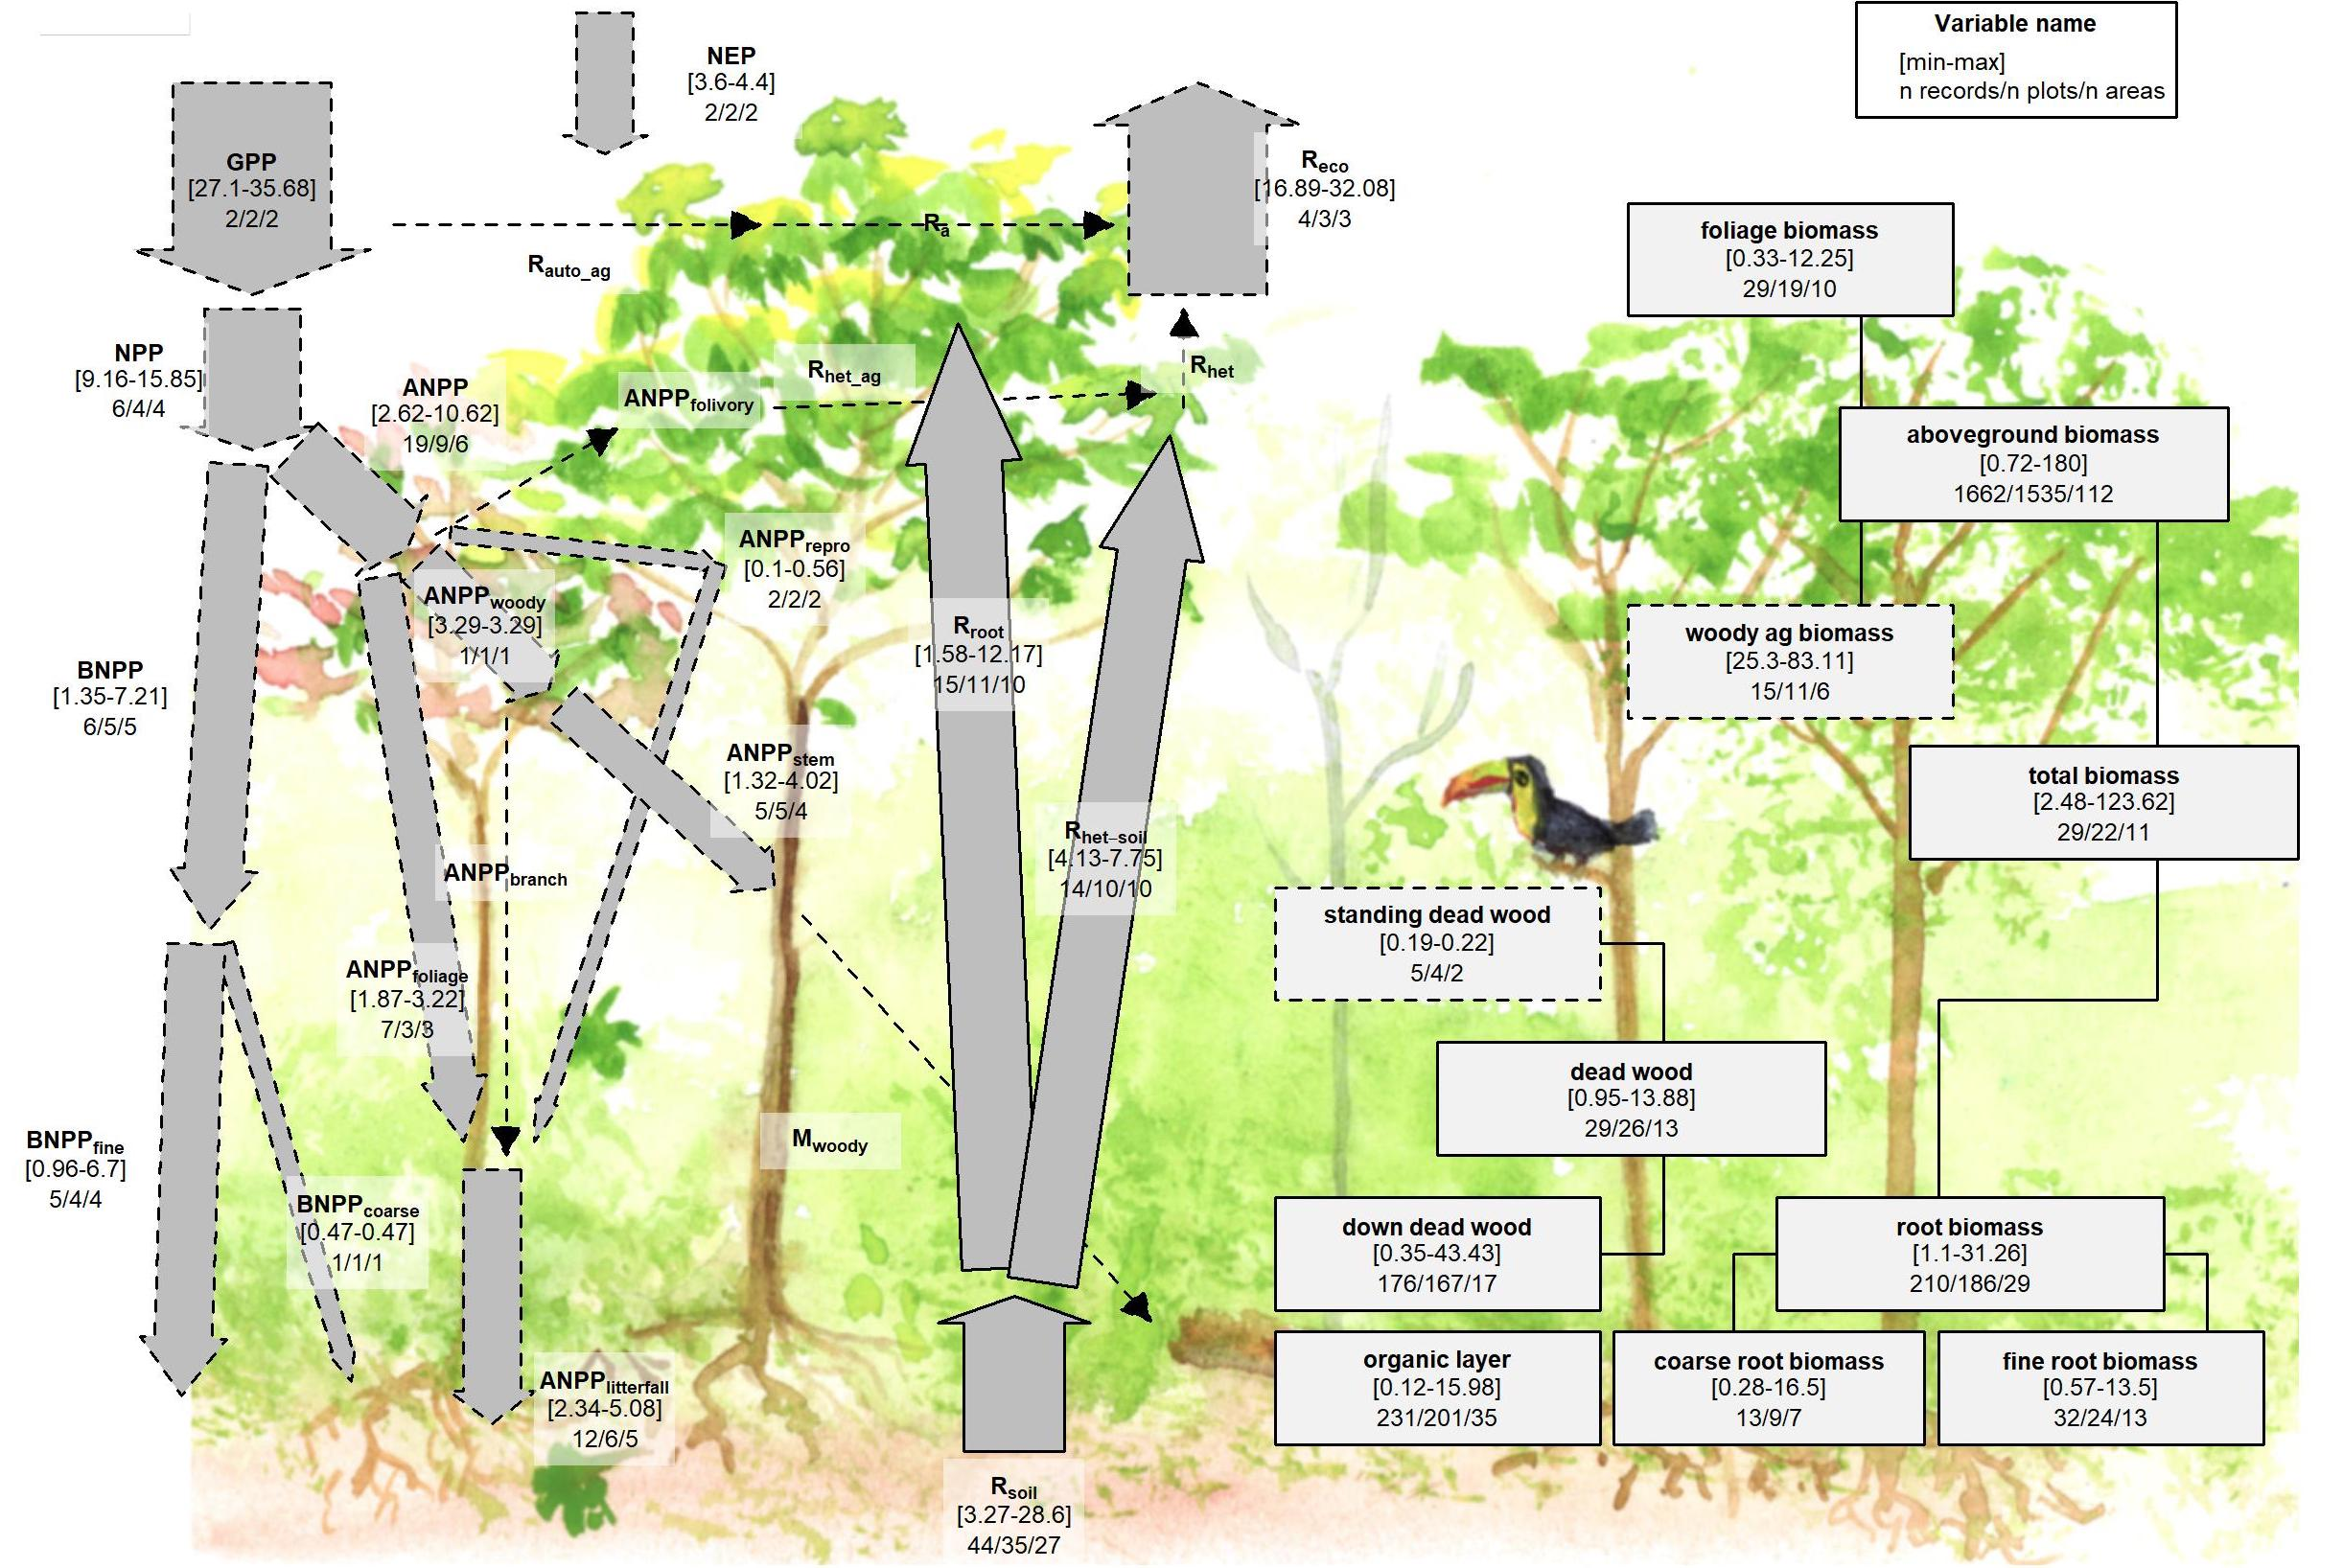
\includegraphics[width=0.84\linewidth]{tables_figures/C_cycle_diagrams/Tropical_broadleaf_YOUNG} 

}

\caption{C cycle diagram for young tropical broadleaf forests. Arrows indicate fluxes (Mg C ha$^{-1}$ yr$^{-1}$); boxes indicate stocks (Mg C ha$^{-1}$), with variables as defined in Table 1. Presented are observed ranges, where geographically distinct areas are treated as the unit of replication. Note that variables differ in geographical and age representation, resulting in potential imbalances (Figs. S5-S30). All units are Mg C ha$^{-1}$ yr$^{-1}$ (fluxes) or Mg C ha$^{-1}$ (stocks). Dashed shape outlines indicate variables with records from <7 distinct geographic areas, and dashed arrows indicate fluxes with no data. To illustrate the magnitude of different fluxes, arrow width is proportional to the square root of the mean of the corresponding flux.}\label{fig:unnamed-chunk-4}
\end{figure}

\hypertarget{figure-s2.-c-cycle-diagram-for-young-temperate-broadleaf-forests.}{%
\subsection{Figure S2. C cycle diagram for young temperate broadleaf
forests.}\label{figure-s2.-c-cycle-diagram-for-young-temperate-broadleaf-forests.}}

\begin{figure}[H]

{\centering 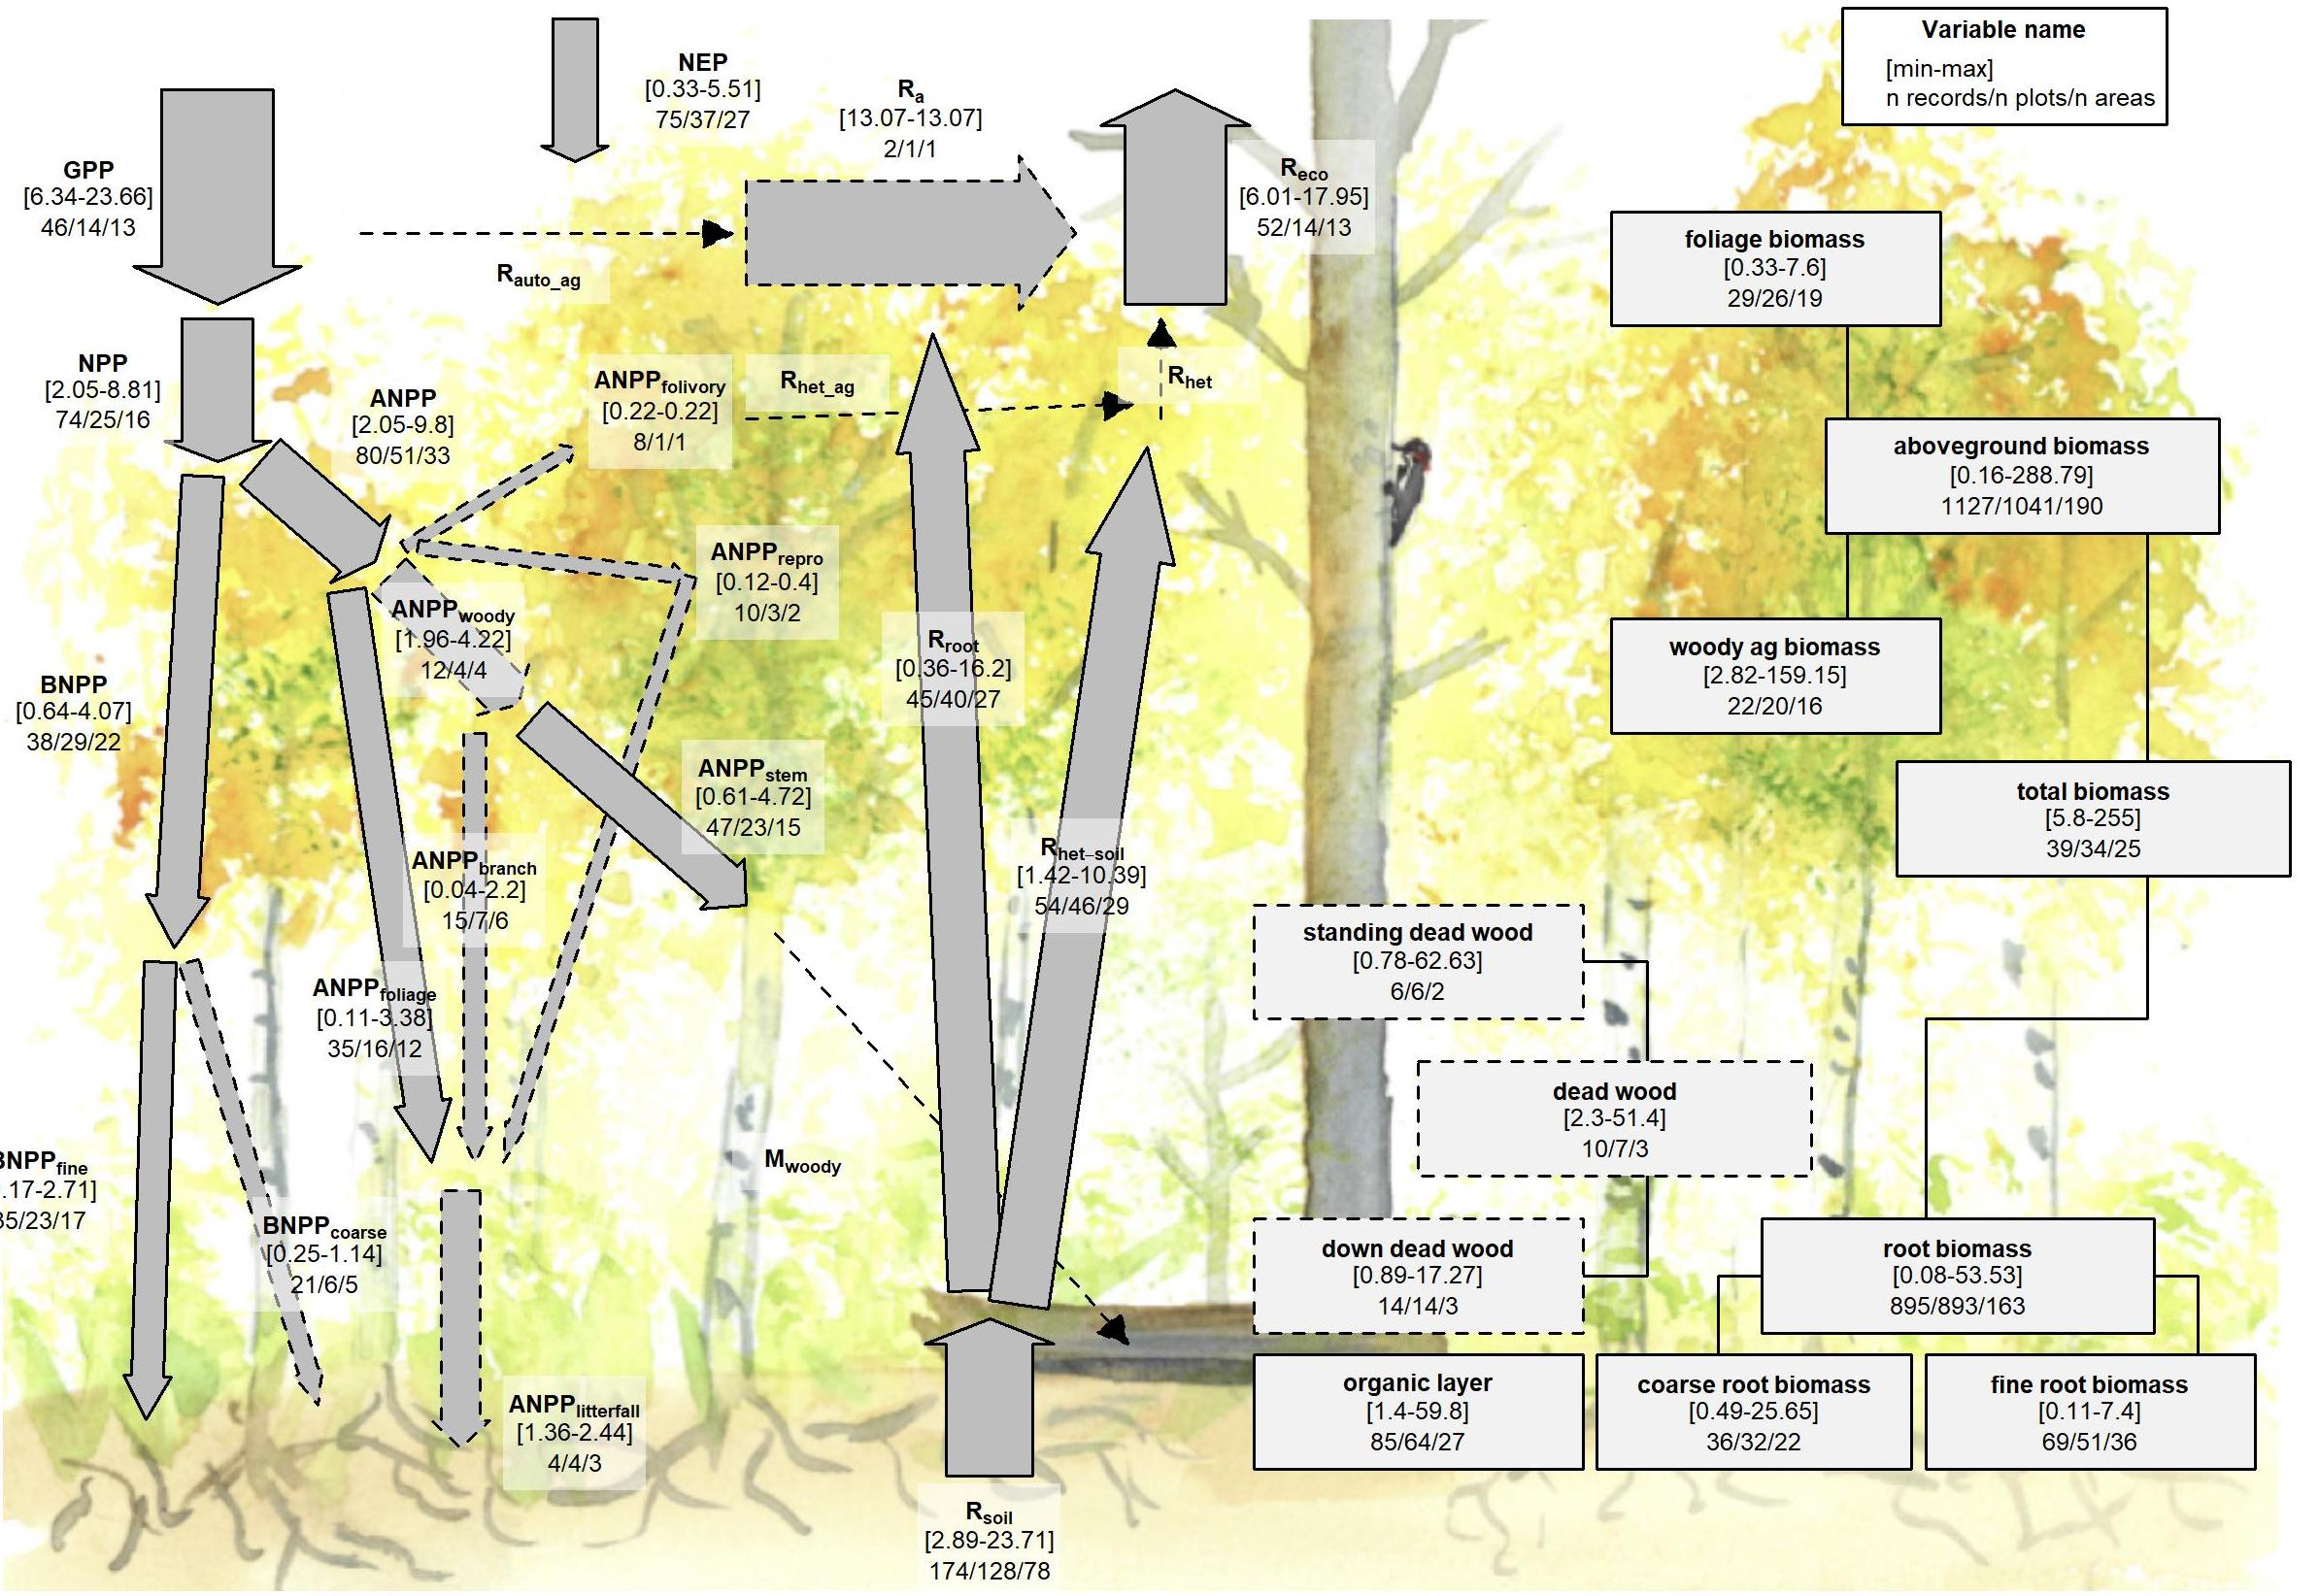
\includegraphics[width=0.84\linewidth]{tables_figures/C_cycle_diagrams/Temperate_broadleaf_YOUNG} 

}

\caption{C cycle diagram for young temperate broadleaf forests. Arrows indicate fluxes (Mg C ha$^{-1}$ yr$^{-1}$); boxes indicate stocks (Mg C ha$^{-1}$), with variables as defined in Table 1. Presented are observed ranges, where geographically distinct areas are treated as the unit of replication. Note that variables differ in geographical and age representation, resulting in potential imbalances (Figs. S5-S30). All units are Mg C ha$^{-1}$ yr$^{-1}$ (fluxes) or Mg C ha$^{-1}$ (stocks). Dashed shape outlines indicate variables with records from <7 distinct geographic areas, and dashed arrows indicate fluxes with no data. To illustrate the magnitude of different fluxes, arrow width is proportional to the square root of the mean of the corresponding flux.}\label{fig:unnamed-chunk-5}
\end{figure}

\hypertarget{figure-s3.-c-cycle-diagram-for-young-temperate-conifer-forests.}{%
\subsection{Figure S3. C cycle diagram for young temperate conifer
forests.}\label{figure-s3.-c-cycle-diagram-for-young-temperate-conifer-forests.}}

\begin{figure}[H]

{\centering 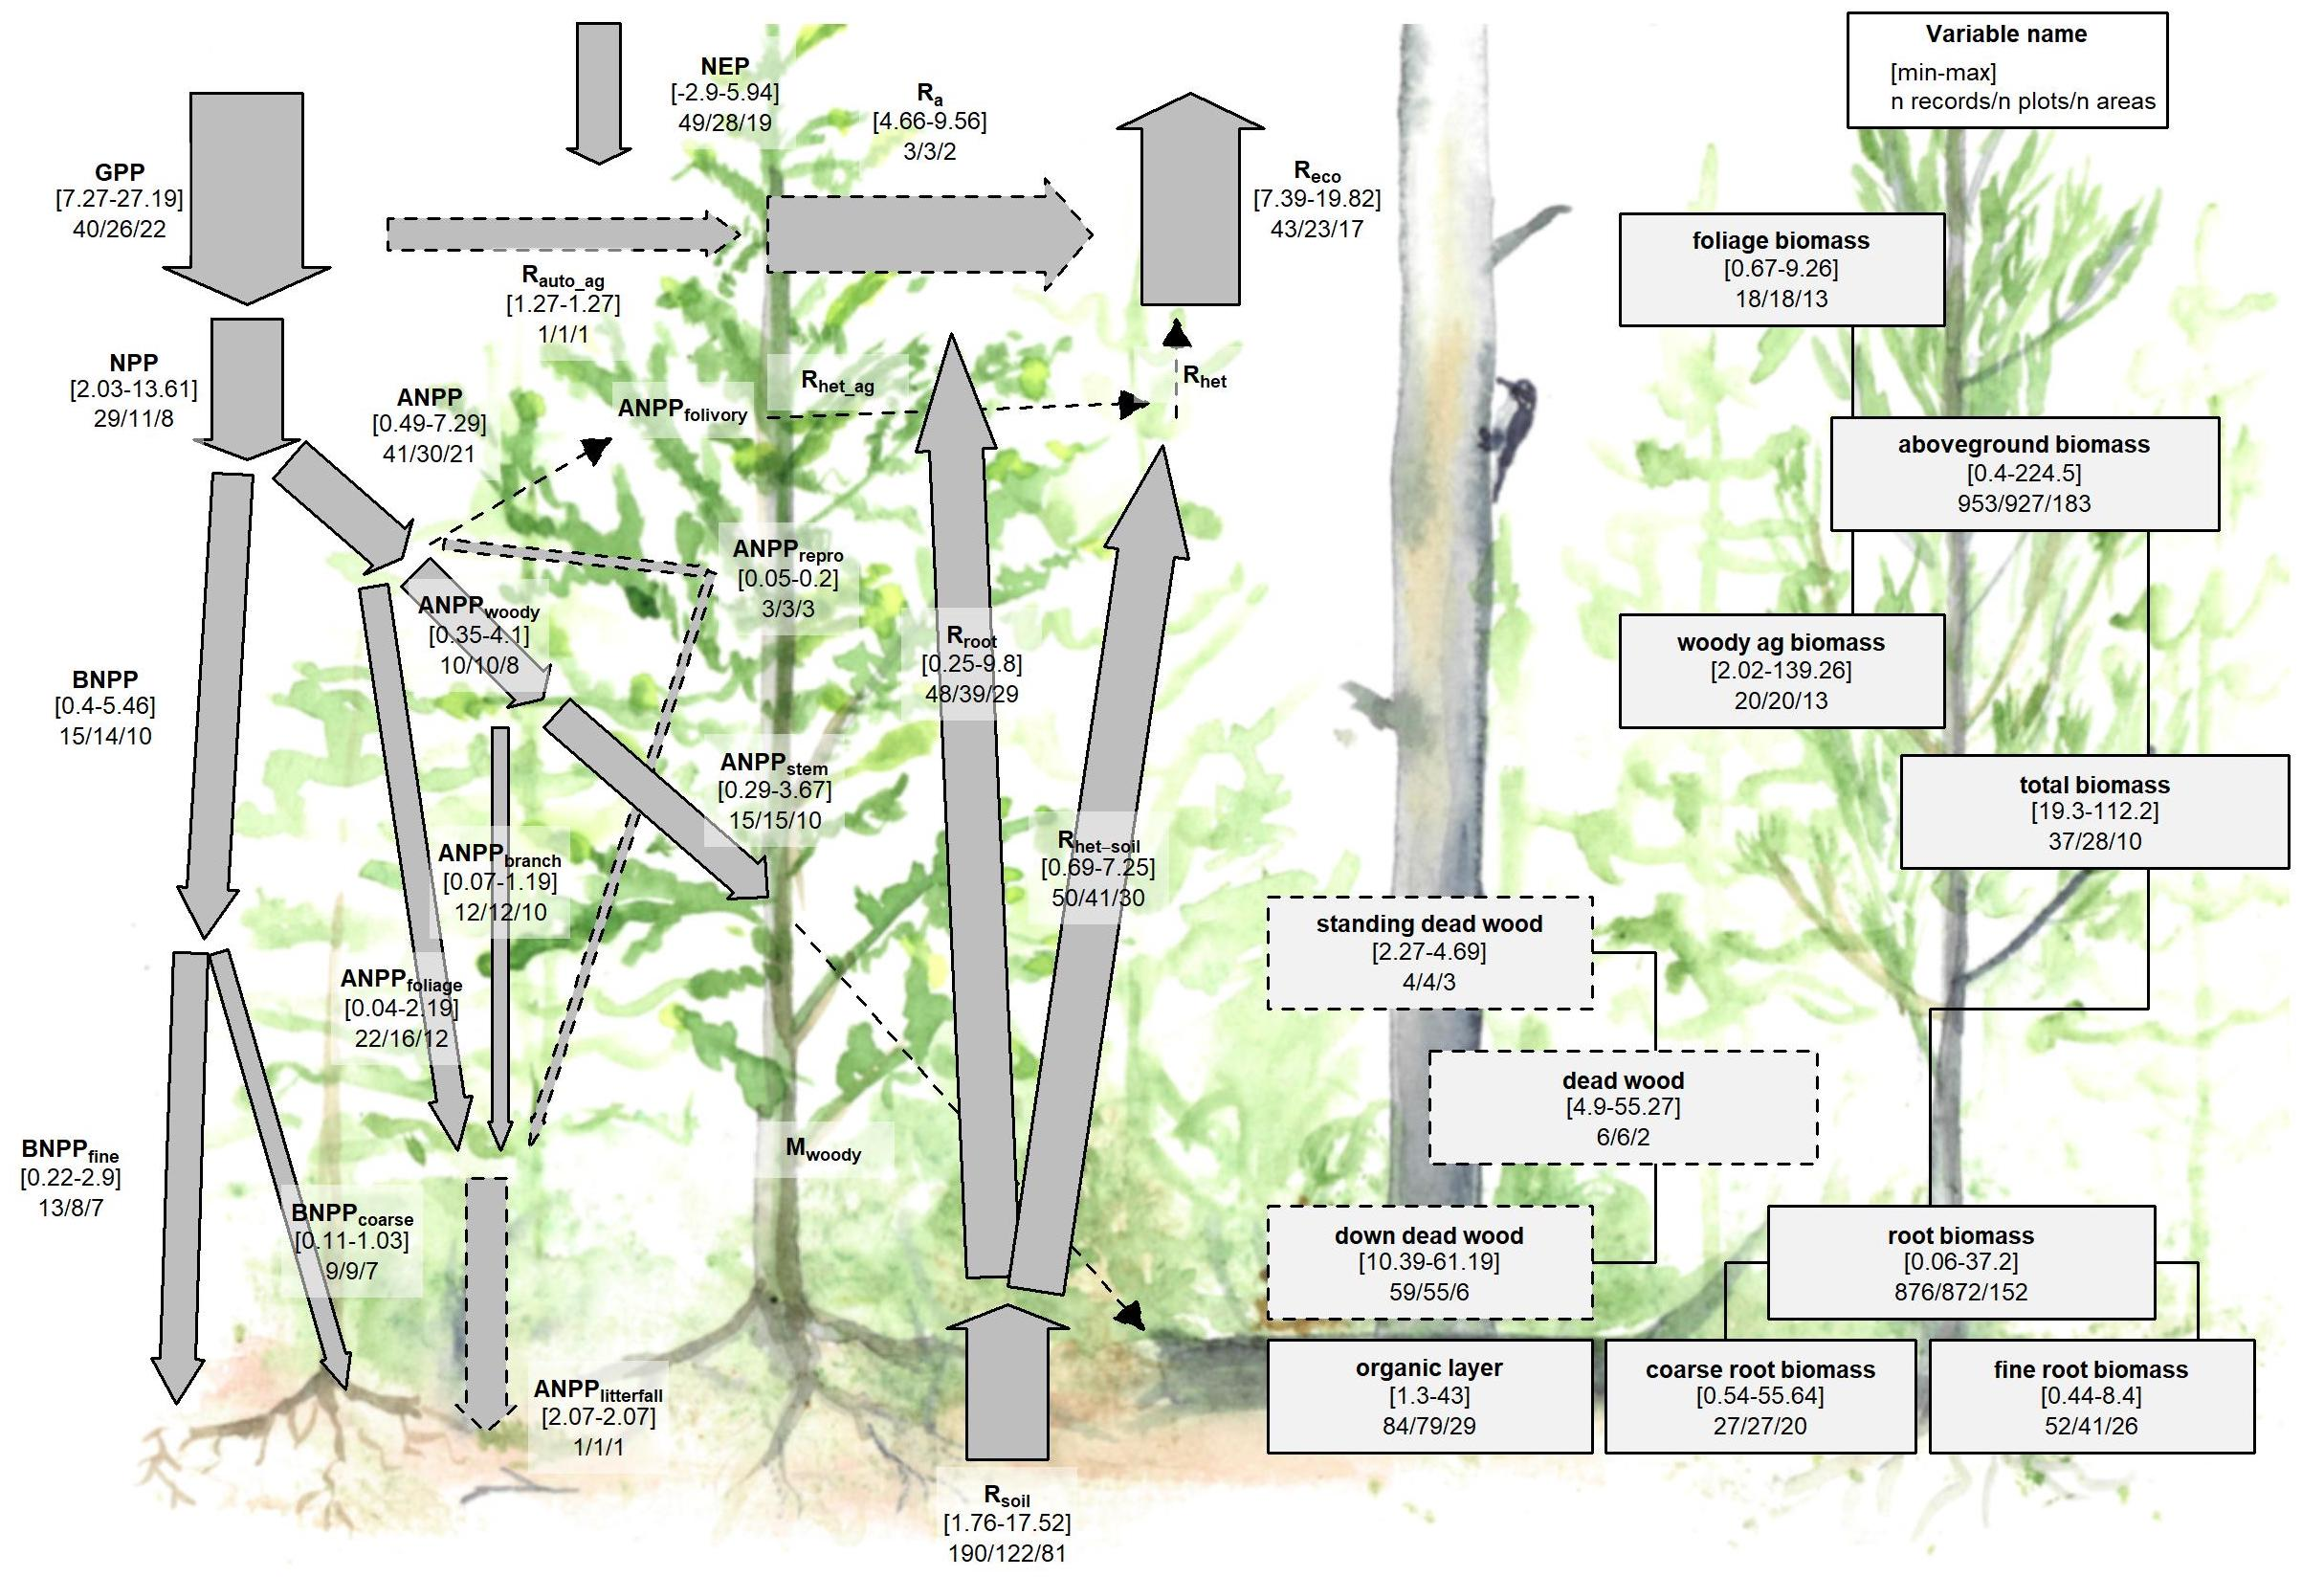
\includegraphics[width=0.84\linewidth]{tables_figures/C_cycle_diagrams/Temperate_conifer_YOUNG} 

}

\caption{ C cycle diagram for young temperate conifer forests. Arrows indicate fluxes (Mg C ha$^{-1}$ yr$^{-1}$); boxes indicate stocks (Mg C ha$^{-1}$), with variables as defined in Table 1. Presented are observed ranges, where geographically distinct areas are treated as the unit of replication. Note that variables differ in geographical and age representation, resulting in potential imbalances (Figs. S5-S30). All units are Mg C ha$^{-1}$ yr$^{-1}$ (fluxes) or Mg C ha$^{-1}$ (stocks). Dashed shape outlines indicate variables with records from <7 distinct geographic areas, and dashed arrows indicate fluxes with no data. To illustrate the magnitude of different fluxes, arrow width is proportional to the square root of the mean of the corresponding flux.}\label{fig:unnamed-chunk-6}
\end{figure}

\hypertarget{figure-s4.-c-cycle-diagram-for-young-boreal-conifer-forests.}{%
\subsection{Figure S4. C cycle diagram for young boreal conifer
forests.}\label{figure-s4.-c-cycle-diagram-for-young-boreal-conifer-forests.}}

\begin{figure}[H]

{\centering 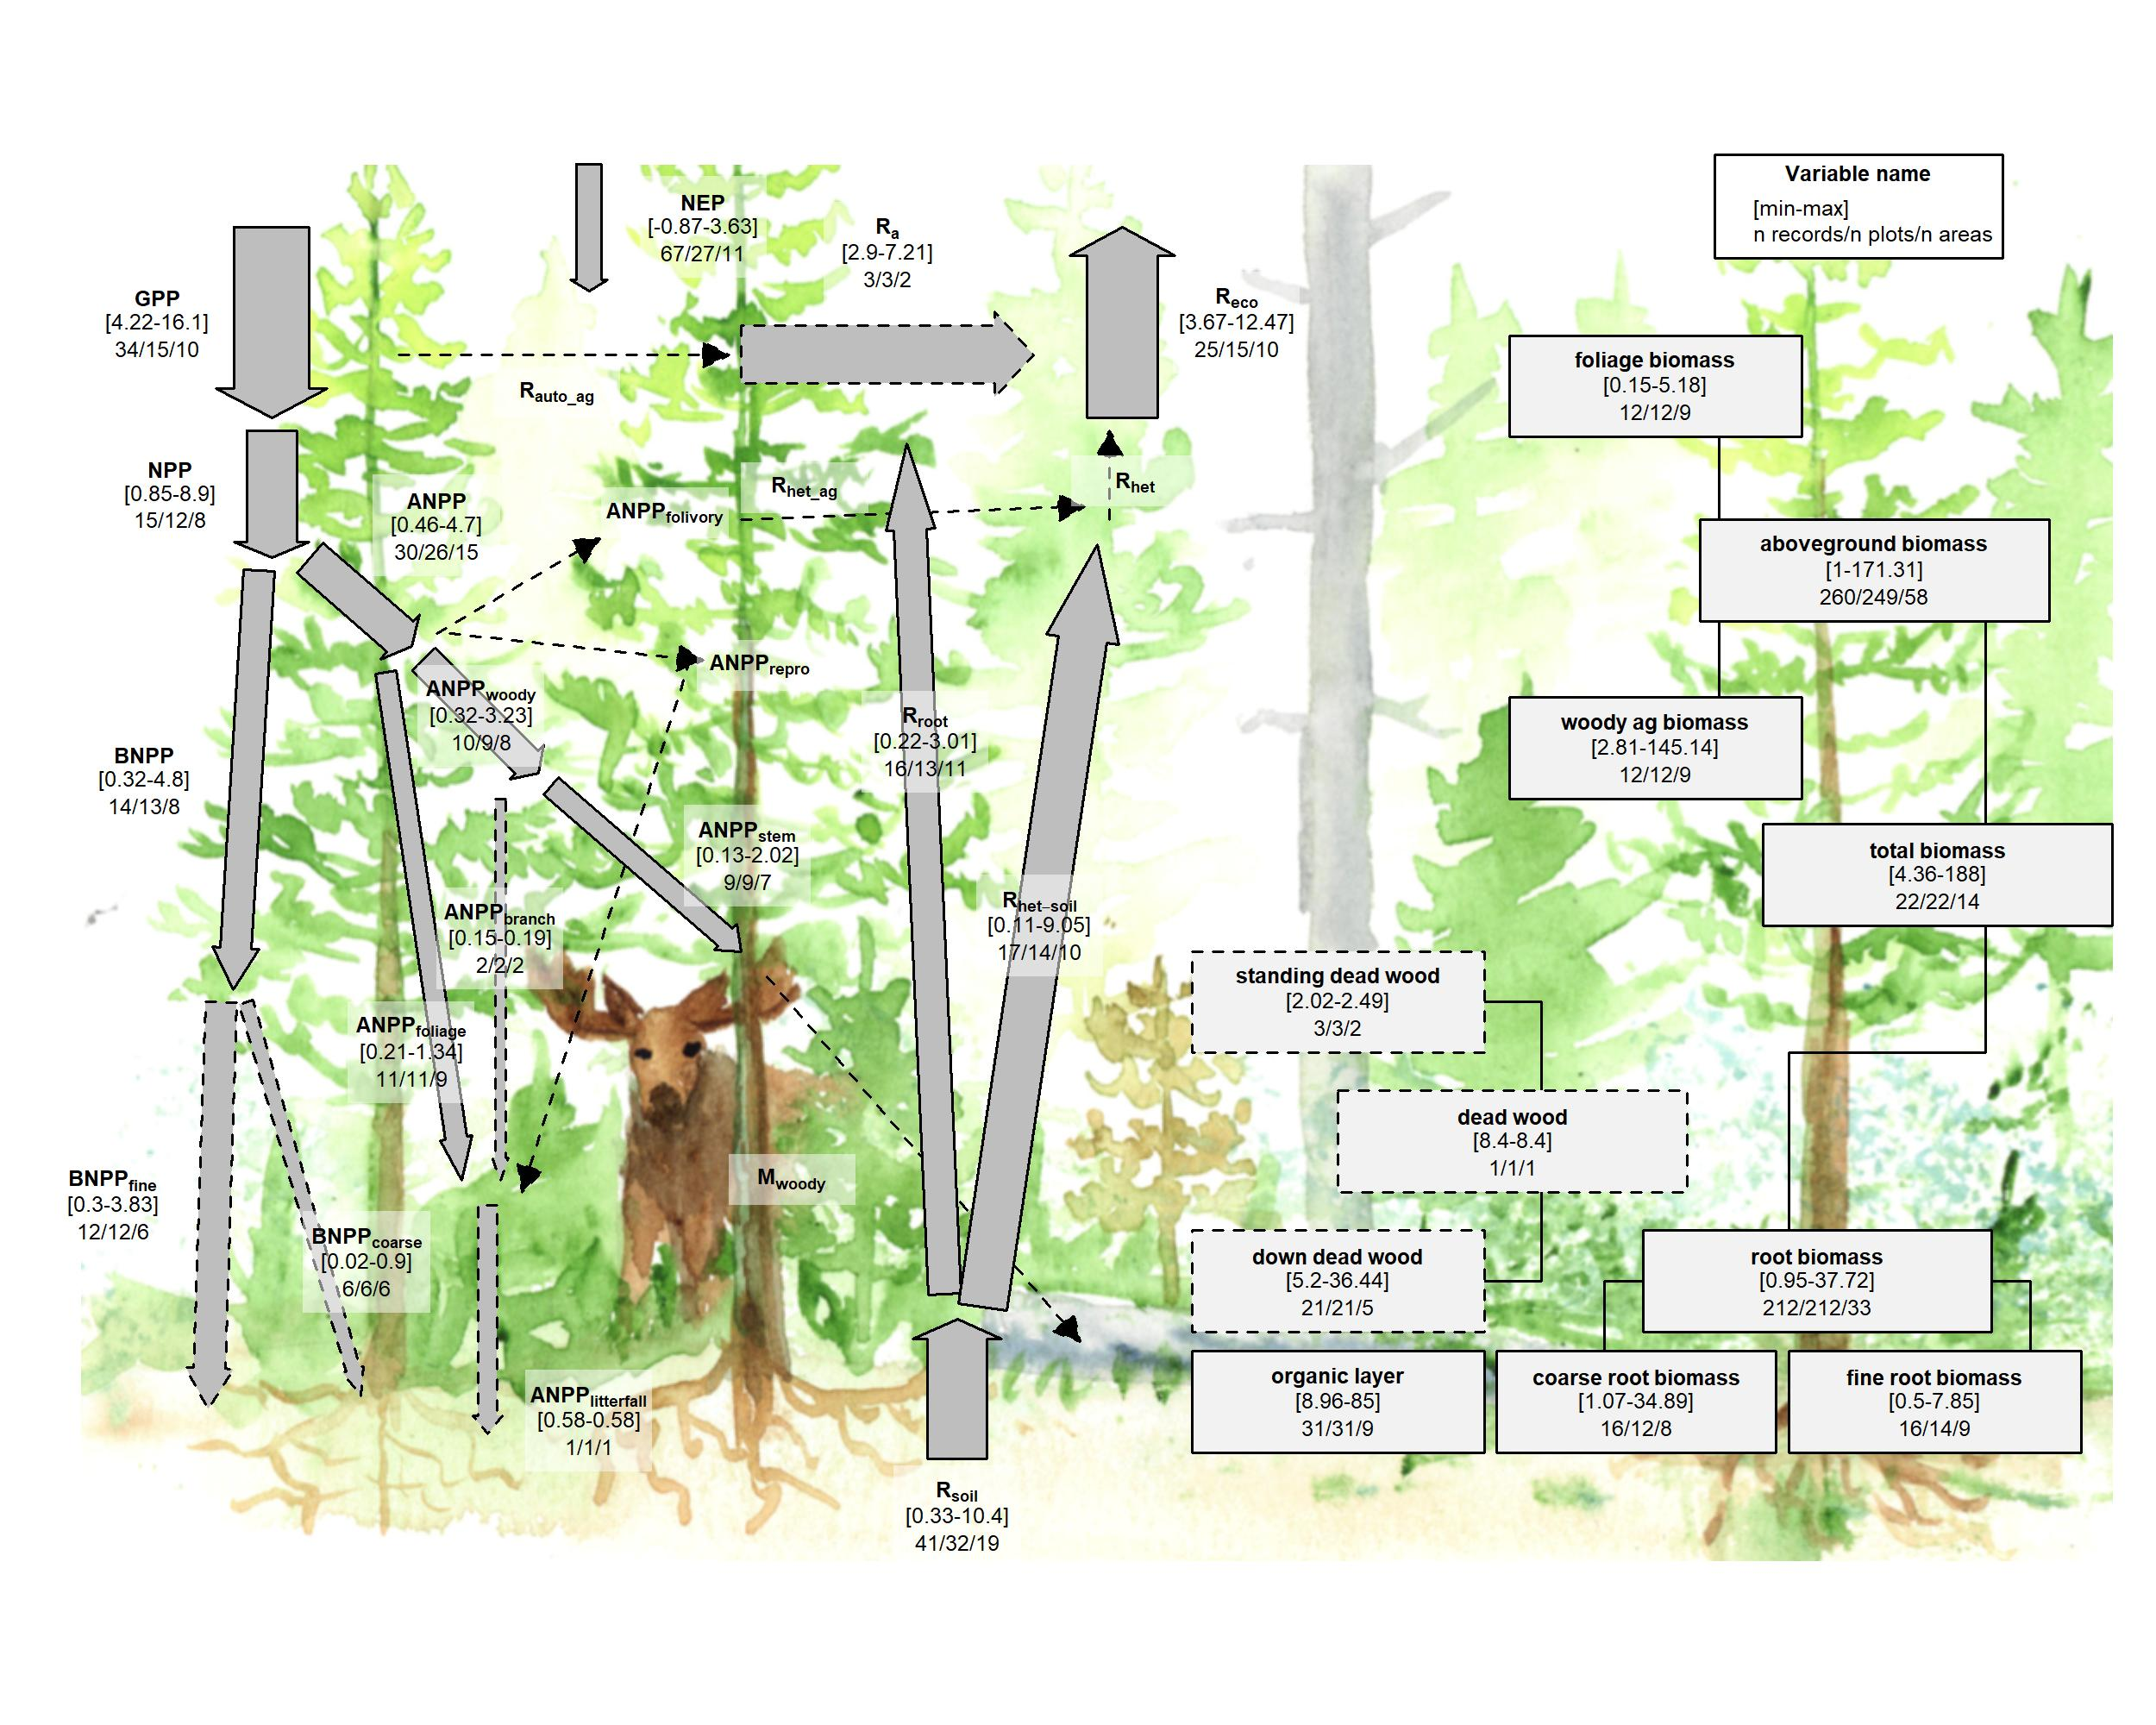
\includegraphics[width=0.84\linewidth]{tables_figures/C_cycle_diagrams/Boreal_conifer_YOUNG} 

}

\caption{C cycle diagram for young boreal conifer forests. Arrows indicate fluxes (Mg C ha$^{-1}$ yr$^{-1}$); boxes indicate stocks (Mg C ha$^{-1}$), with variables as defined in Table 1. Presented are observed ranges, where geographically distinct areas are treated as the unit of replication. Note that variables differ in geographical and age representation, resulting in potential imbalances (Figs. S5-S30). All units are Mg C ha$^{-1}$ yr$^{-1}$ (fluxes) or Mg C ha$^{-1}$ (stocks). Dashed shape outlines indicate variables with records from <7 distinct geographic areas, and dashed arrows indicate fluxes with no data. To illustrate the magnitude of different fluxes, arrow width is proportional to the square root of the mean of the corresponding flux.}\label{fig:unnamed-chunk-7}
\end{figure}
\end{landscape}

\newpage

\hypertarget{figure-s5.-age-trends-and-biome-differences-for-nep}{%
\subsection{\texorpdfstring{Figure S5. Age trends and biome differences
for
\(NEP\)}{Figure S5. Age trends and biome differences for NEP}}\label{figure-s5.-age-trends-and-biome-differences-for-nep}}

\begin{figure}[H]

{\centering 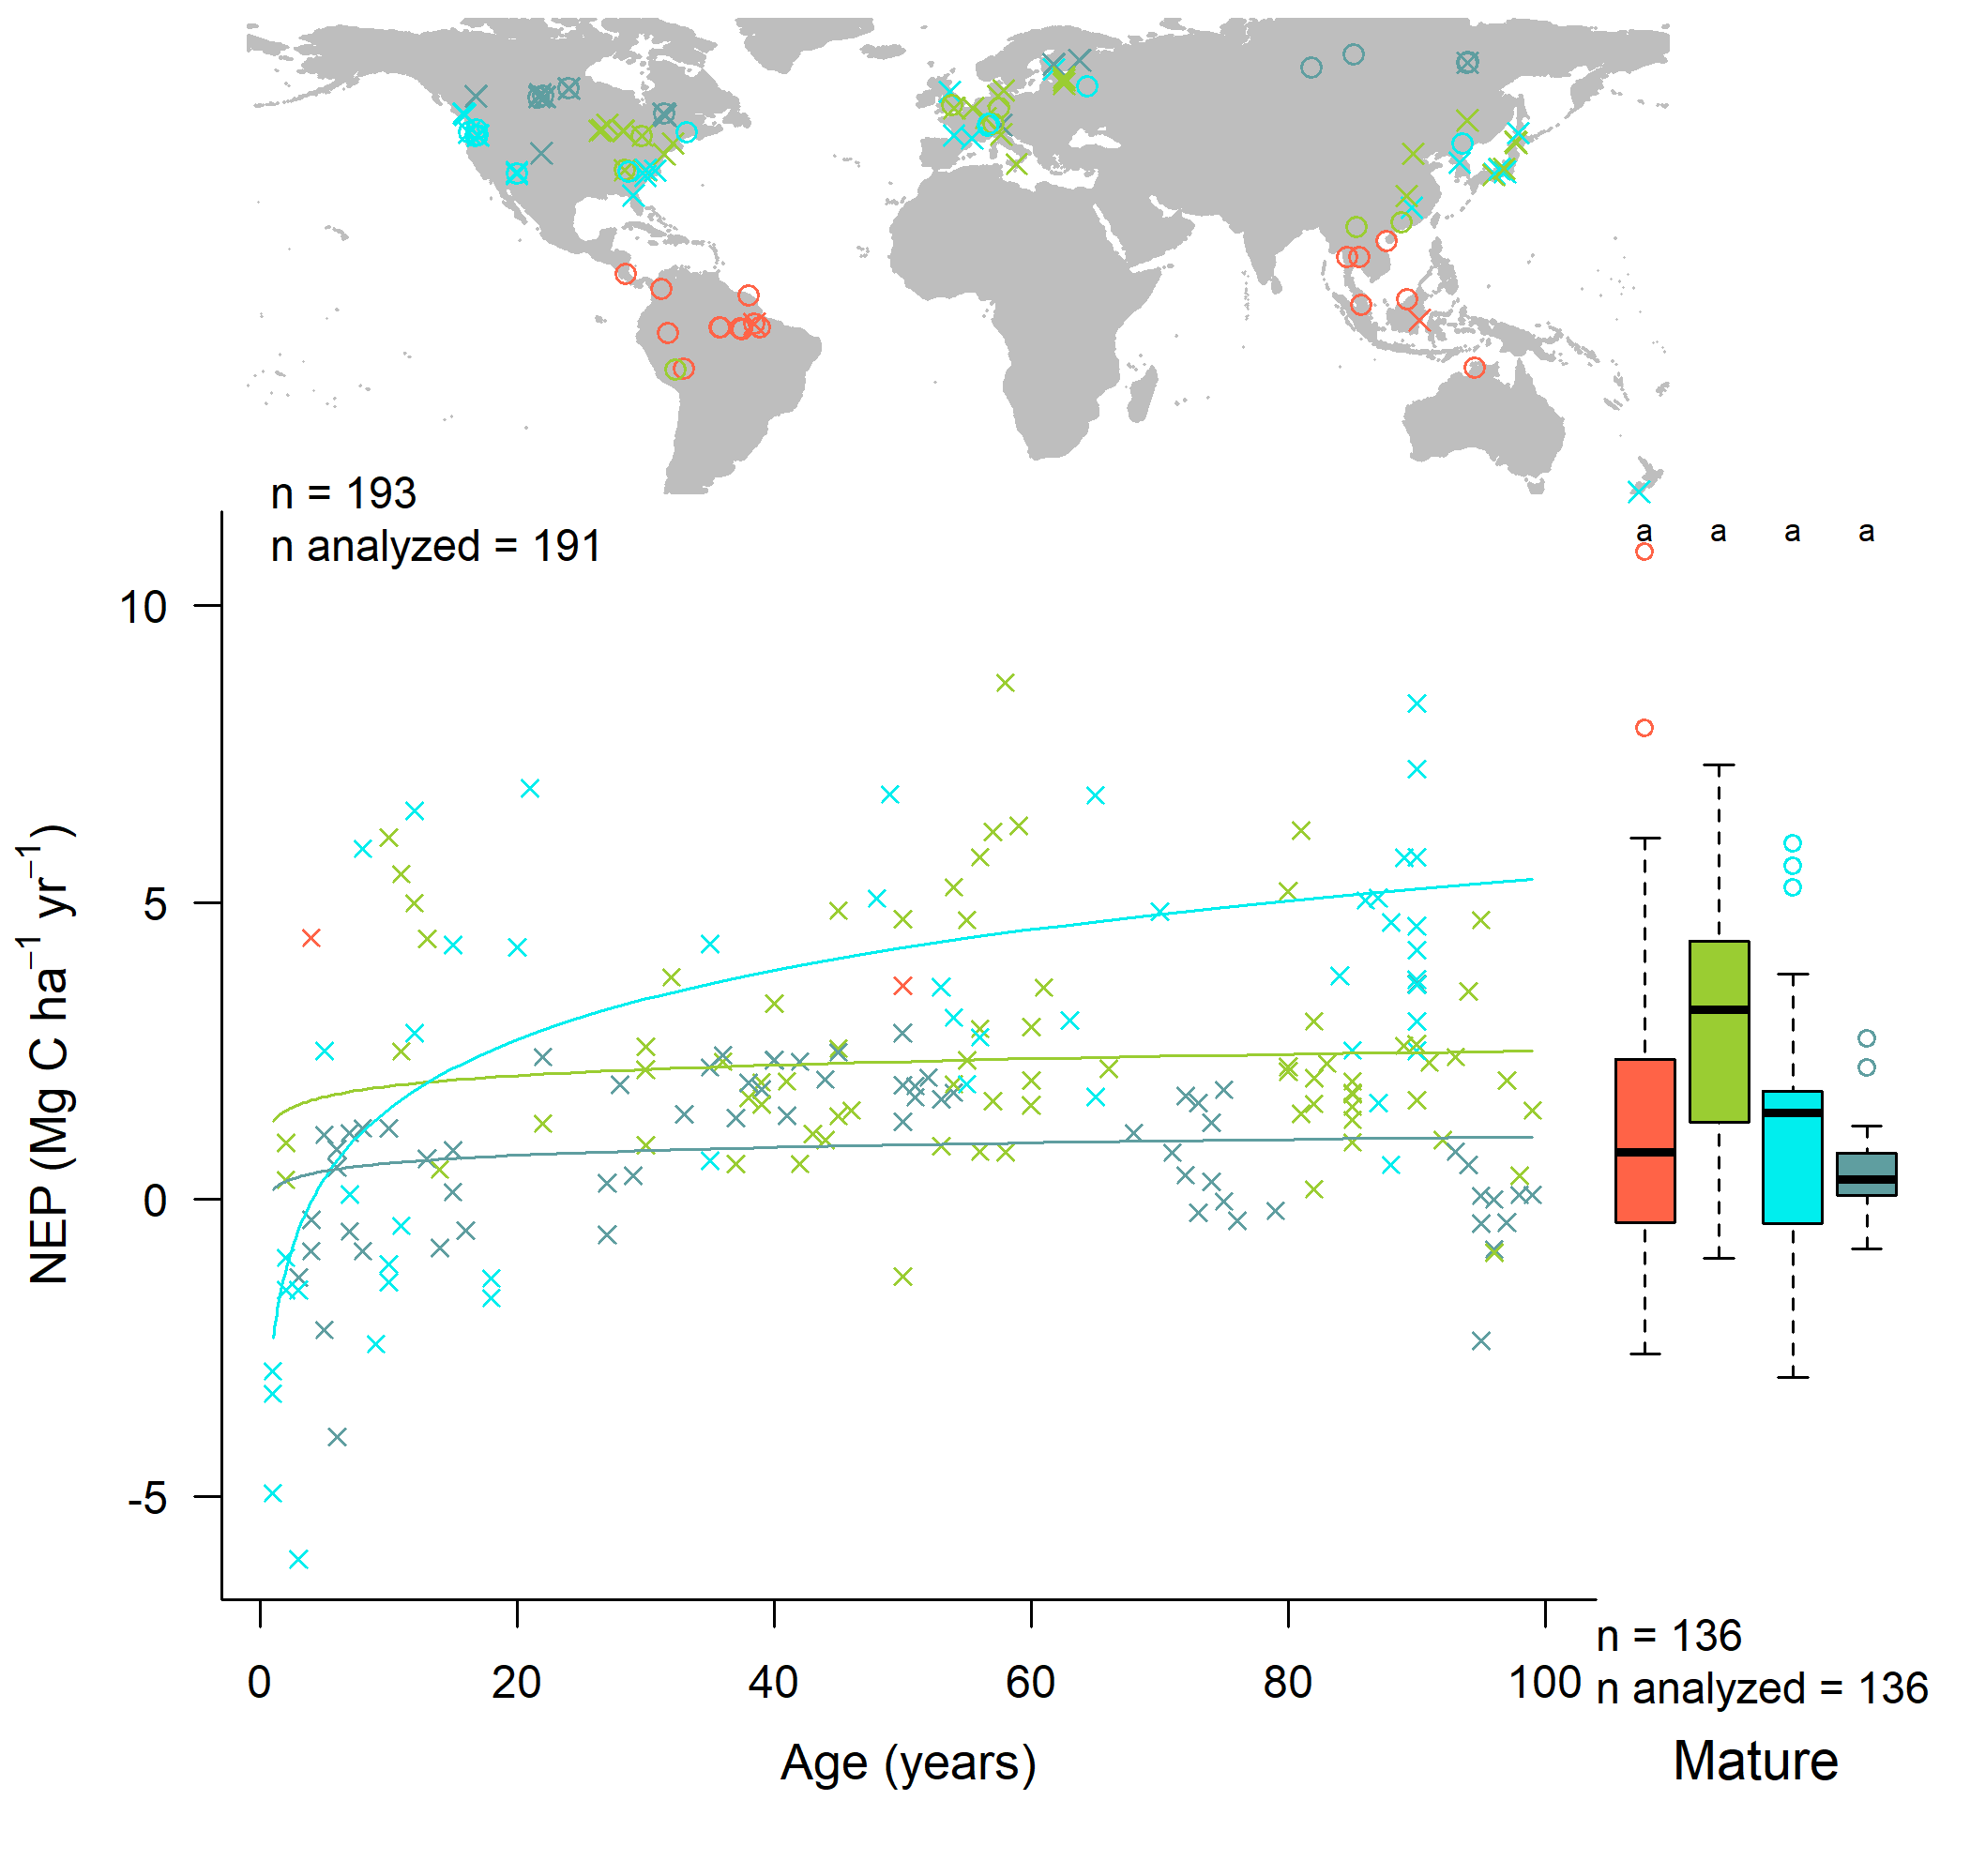
\includegraphics[width=1\linewidth]{tables_figures/age_trends/NEP_with_map} 

}

\caption{Age trends and biome differences for $NEP$. Map shows data sources ('$\times$' and '$\circ$' indicate young and mature stands, respectively). In each panel, the left scatterplot shows age trends in forests up to 100 years old, as characterized by a linear mixed effects model with fixed effects of log10(age) and biome. The fitted line indicates the effect of age (solid lines: significant at p<0.05, dashed lines: non-significant), and non-parallel lines indicate a significant log10(age) $\times$ biome interaction. Boxplot illustrates distribution across mature forests, with different letters indicating significant differences between biomes. Data from biomes that did not meet the sample size criteria (see Methods) are plotted, but lack regression lines (young forests) or test of differences across biomes (mature forests).}\label{fig:unnamed-chunk-8}
\end{figure}

\newpage

\hypertarget{figure-s6.-age-trends-and-biome-differences-for-gpp}{%
\subsection{\texorpdfstring{Figure S6. Age trends and biome differences
for
\(GPP\)}{Figure S6. Age trends and biome differences for GPP}}\label{figure-s6.-age-trends-and-biome-differences-for-gpp}}

\begin{figure}[H]

{\centering 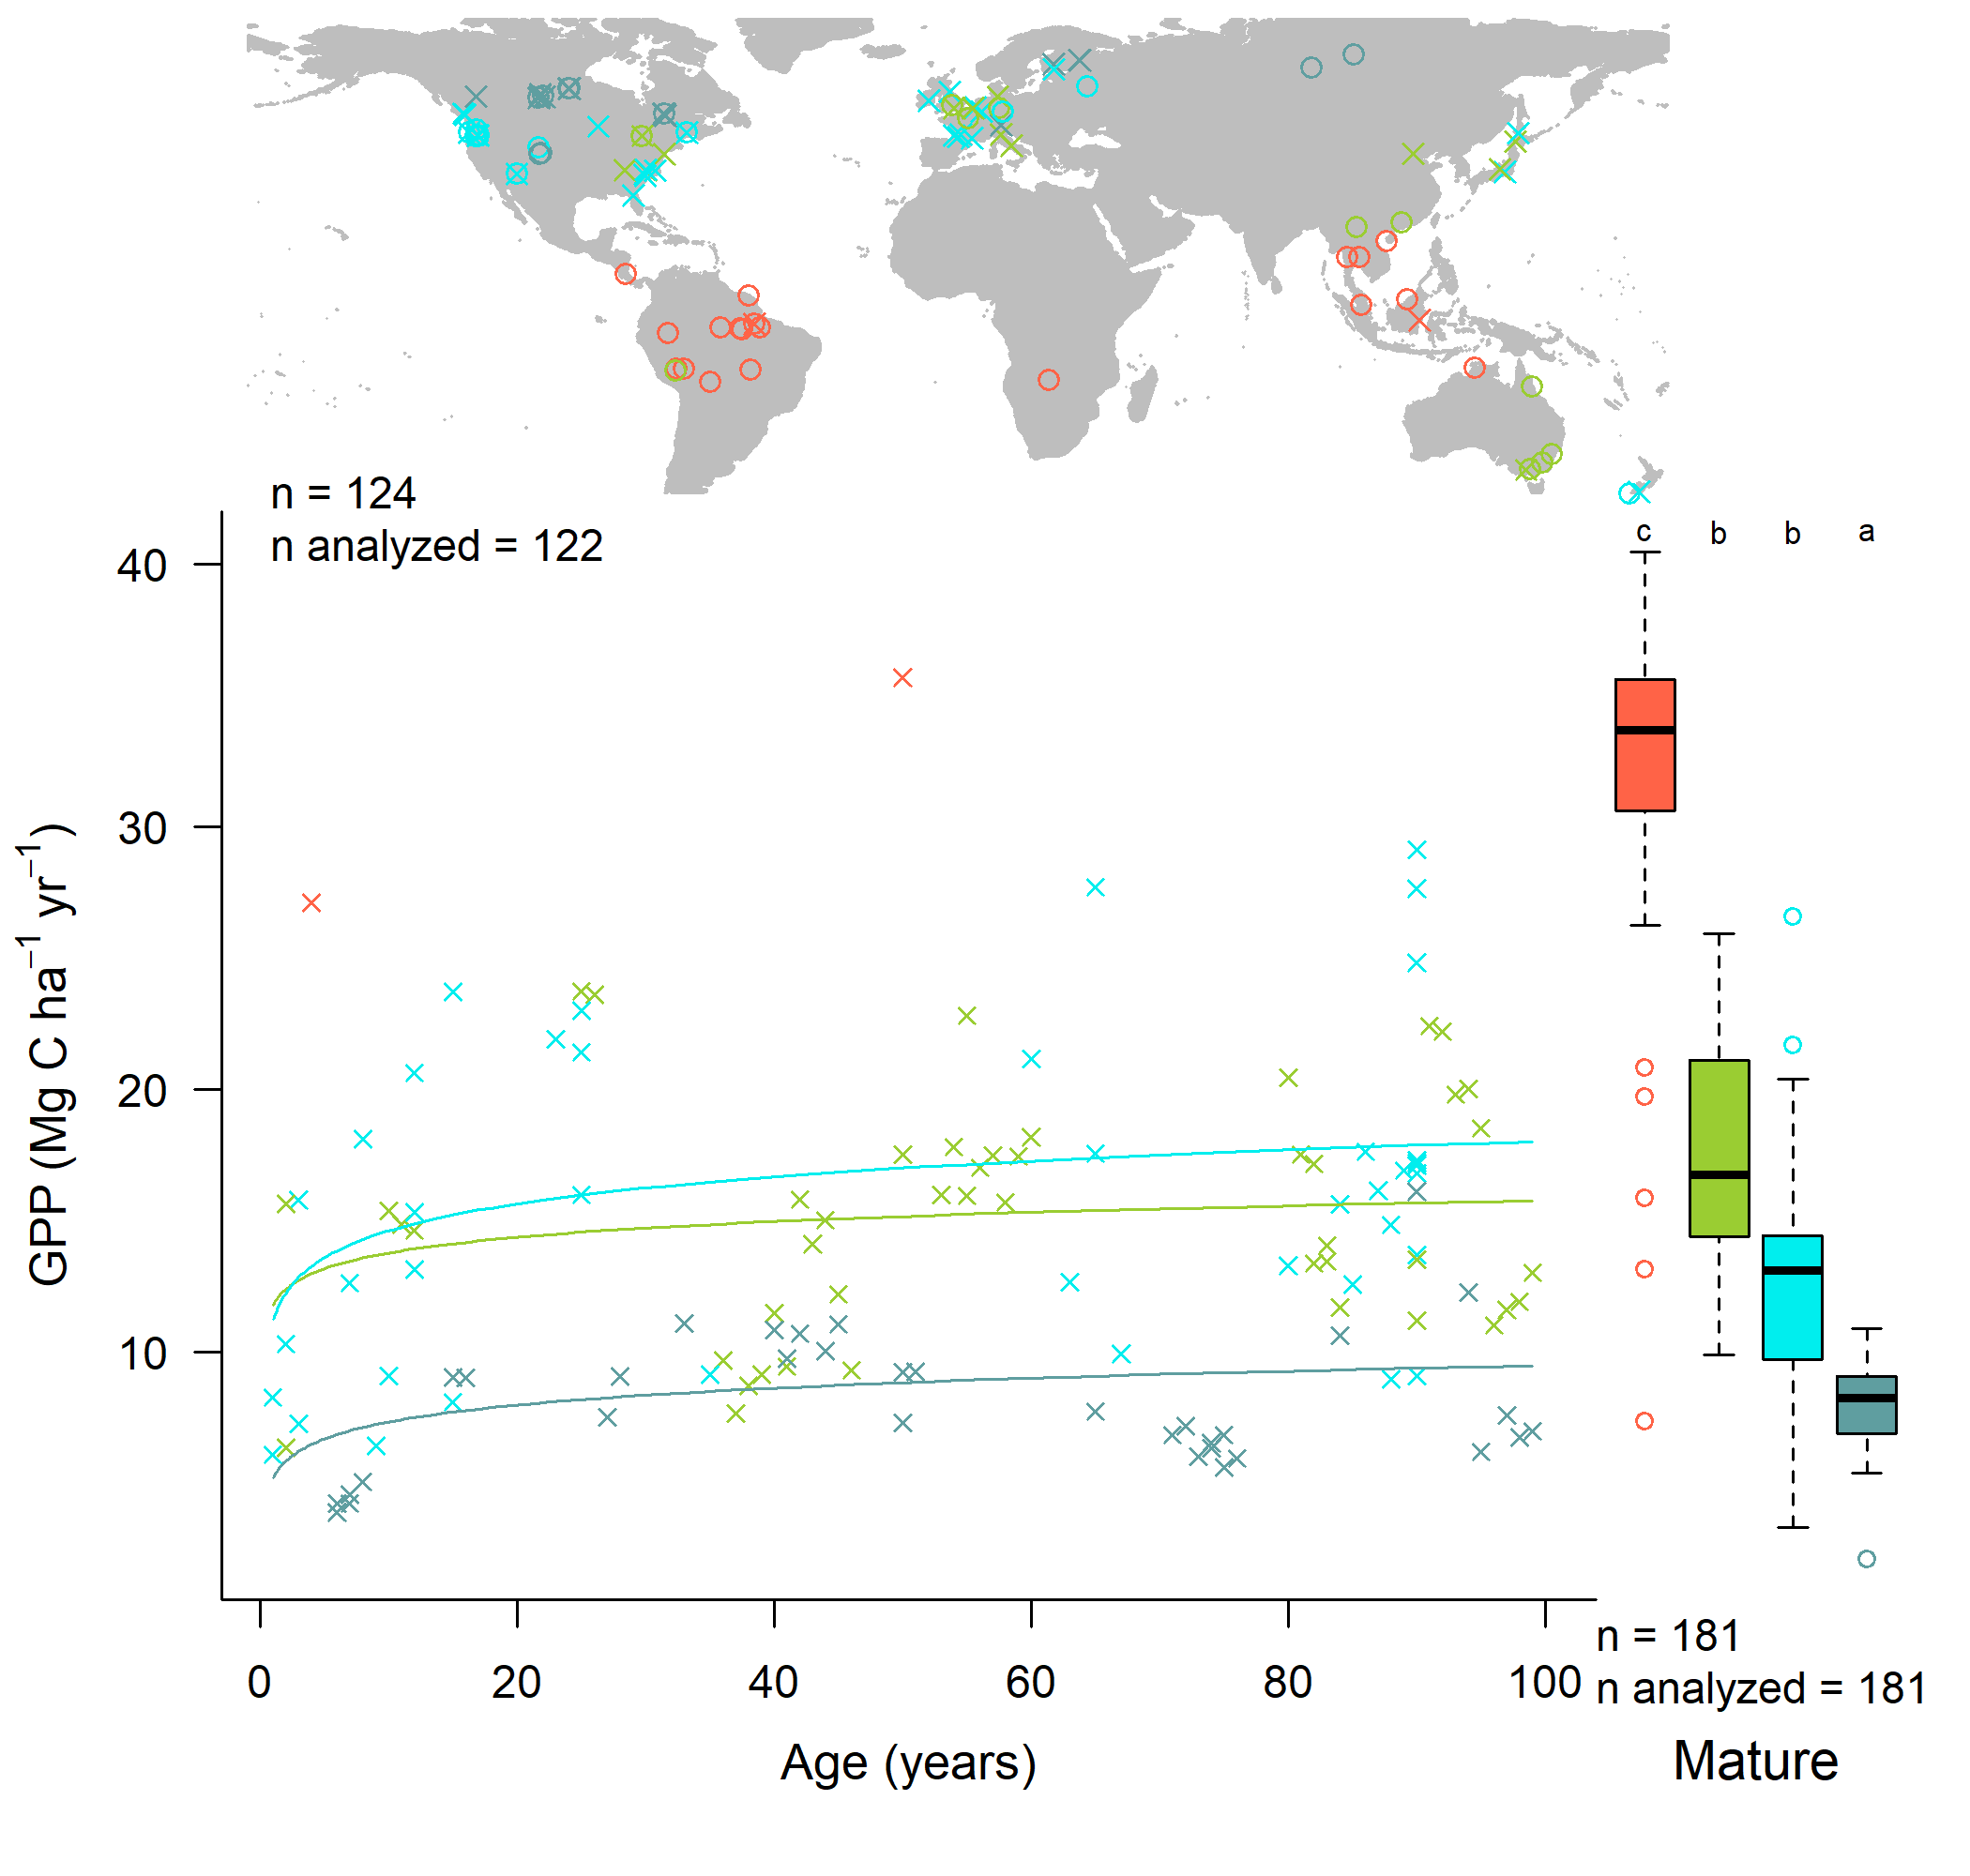
\includegraphics[width=1\linewidth]{tables_figures/age_trends/GPP_with_map} 

}

\caption{Age trends and biome differences for $GPP$. Map shows data sources ('$\times$' and '$\circ$' indicate young and mature stands, respectively). In each panel, the left scatterplot shows age trends in forests up to 100 years old, as characterized by a linear mixed effects model with fixed effects of log10(age) and biome. The fitted line indicates the effect of age (solid lines: significant at p<0.05, dashed lines: non-significant), and non-parallel lines indicate a significant log10(age) $\times$ biome interaction. Boxplot illustrates distribution across mature forests, with different letters indicating significant differences between biomes. Data from biomes that did not meet the sample size criteria (see Methods) are plotted, but lack regression lines (young forests) or test of differences across biomes (mature forests).}\label{fig:unnamed-chunk-9}
\end{figure}

\newpage

\hypertarget{figure-s7.-age-trends-and-biome-differences-for-npp}{%
\subsection{\texorpdfstring{Figure S7. Age trends and biome differences
for
\(NPP\)}{Figure S7. Age trends and biome differences for NPP}}\label{figure-s7.-age-trends-and-biome-differences-for-npp}}

\begin{figure}[H]

{\centering 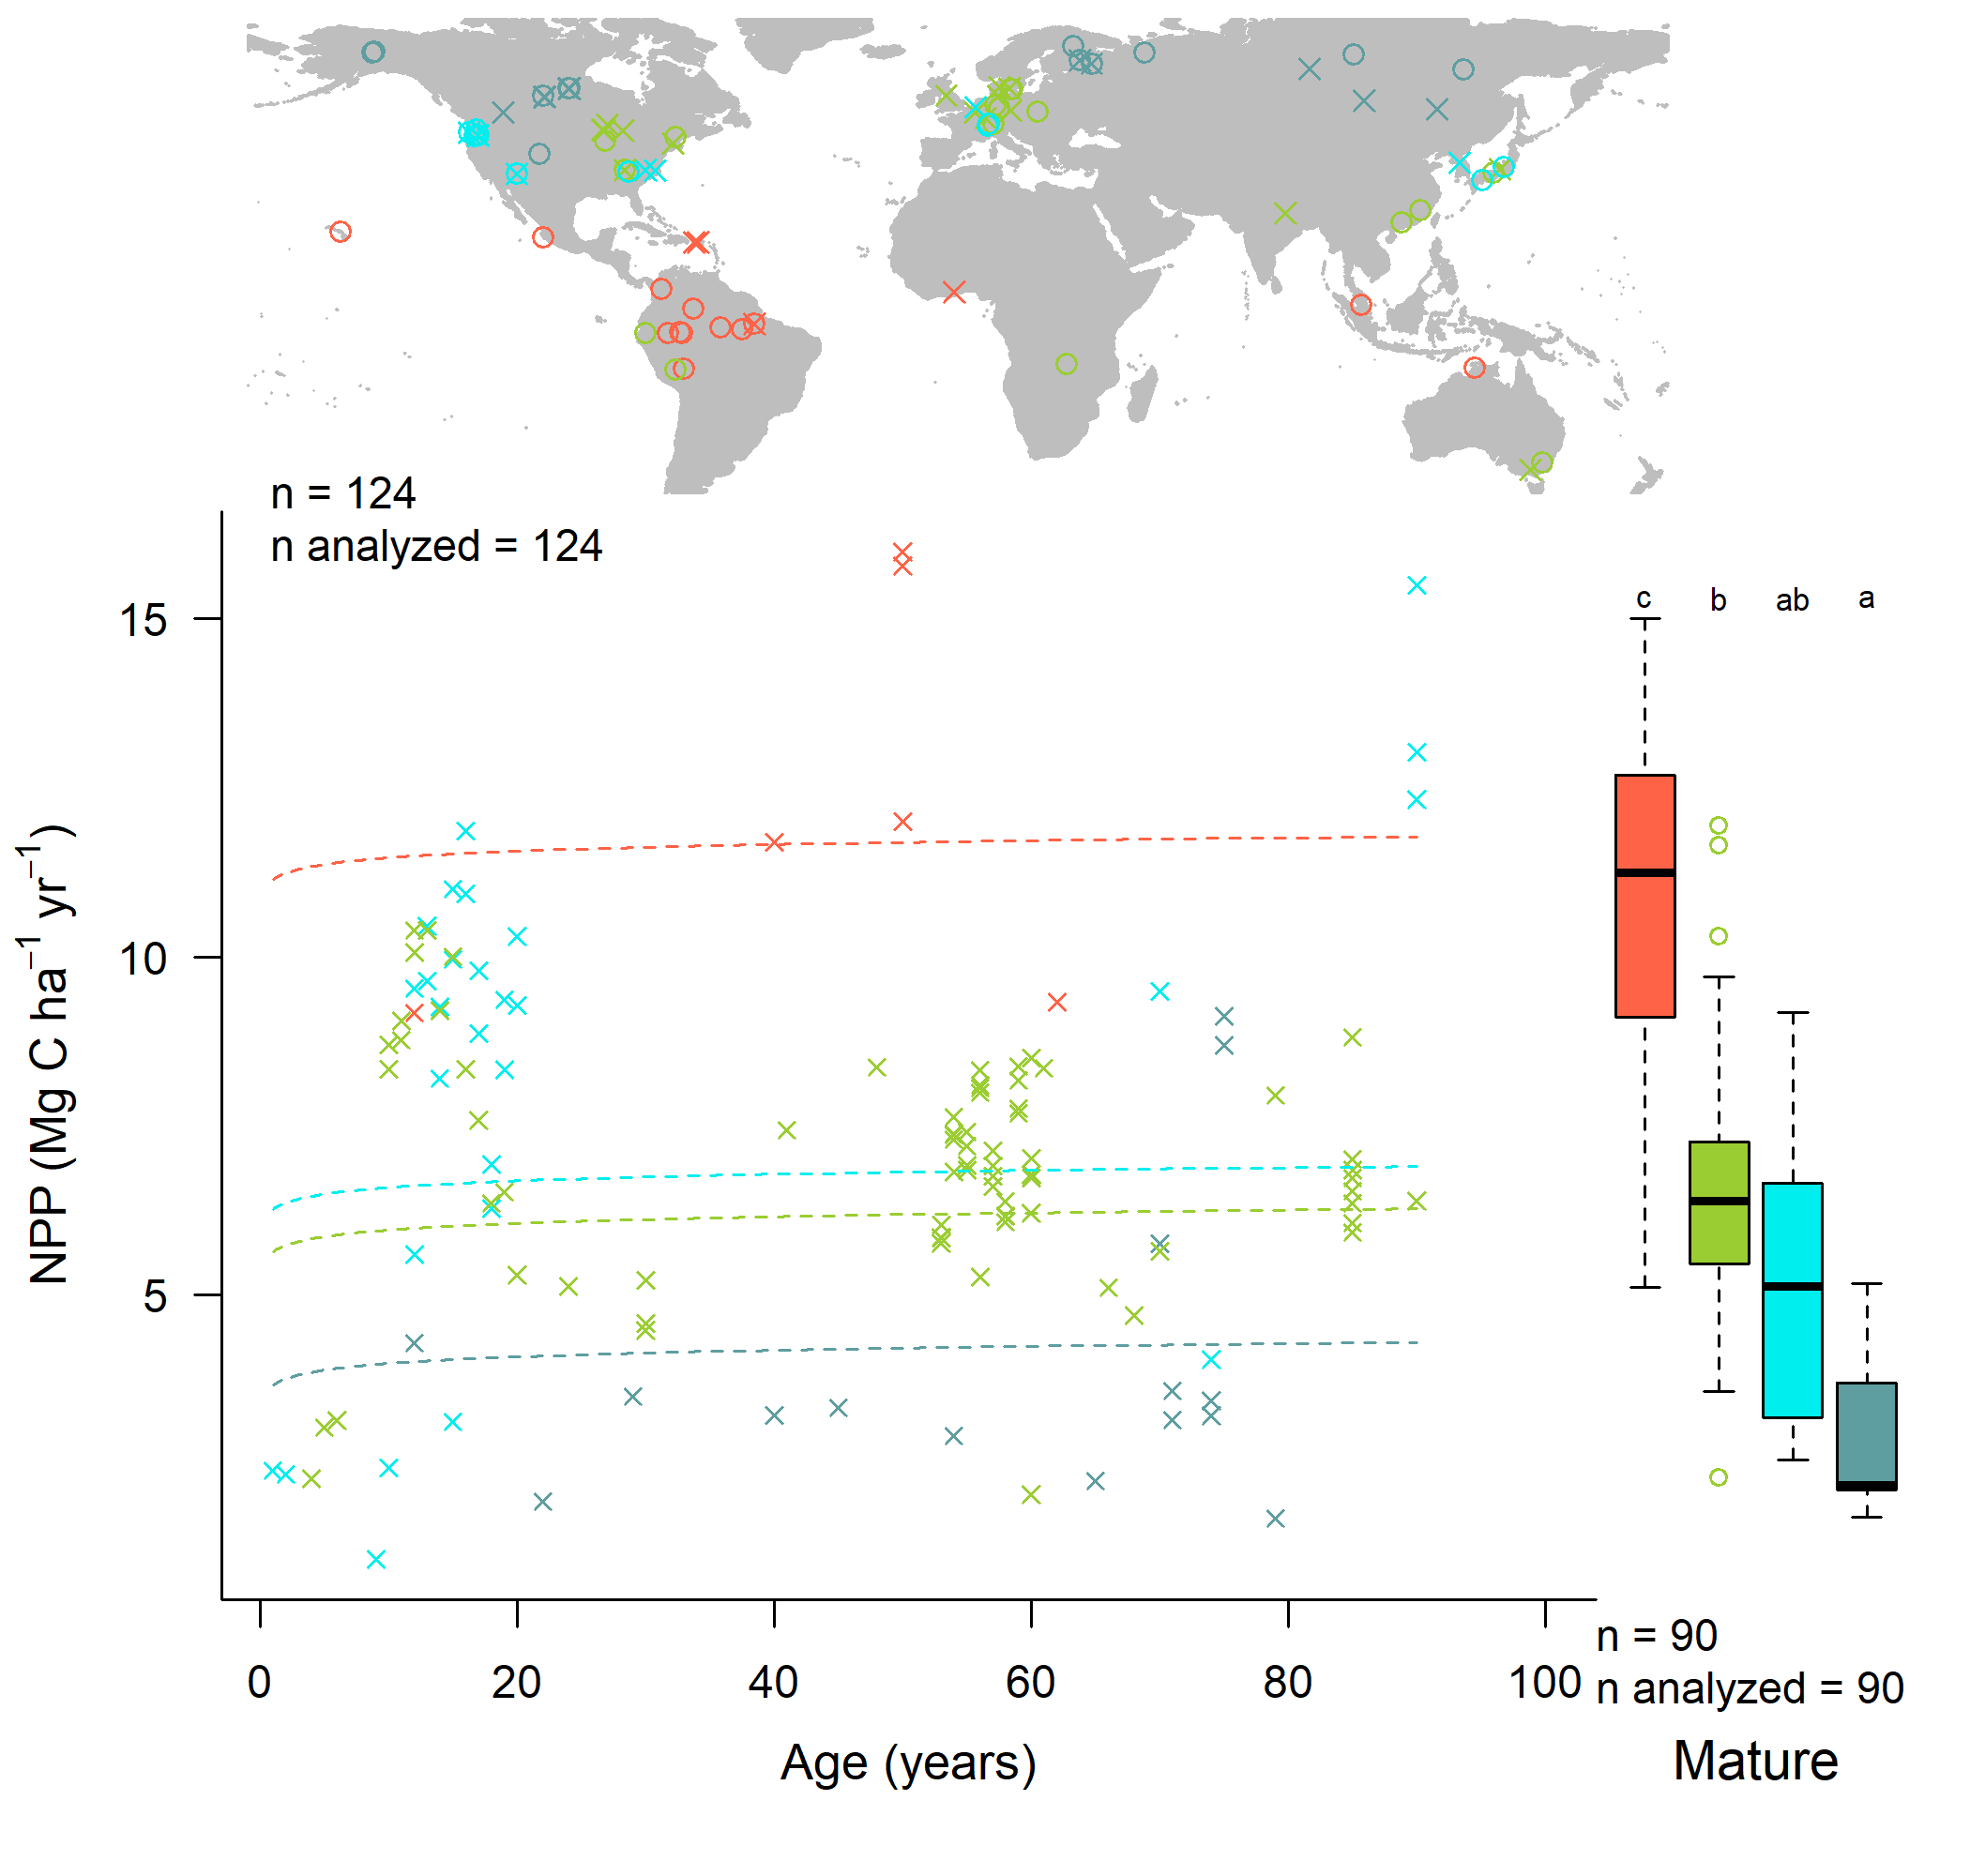
\includegraphics[width=1\linewidth]{tables_figures/age_trends/NPP_with_map} 

}

\caption{Age trends and biome differences for $NPP$. Map shows data sources ('$\times$' and '$\circ$' indicate young and mature stands, respectively). In each panel, the left scatterplot shows age trends in forests up to 100 years old, as characterized by a linear mixed effects model with fixed effects of log10(age) and biome. The fitted line indicates the effect of age (solid lines: significant at p<0.05, dashed lines: non-significant), and non-parallel lines indicate a significant log10(age) $\times$ biome interaction. Boxplot illustrates distribution across mature forests, with different letters indicating significant differences between biomes. Data from biomes that did not meet the sample size criteria (see Methods) are plotted, but lack regression lines (young forests) or test of differences across biomes (mature forests).}\label{fig:unnamed-chunk-10}
\end{figure}

\newpage

\hypertarget{figure-s8.-age-trends-and-biome-differences-for-anpp}{%
\subsection{\texorpdfstring{Figure S8. Age trends and biome differences
for
\(ANPP\)}{Figure S8. Age trends and biome differences for ANPP}}\label{figure-s8.-age-trends-and-biome-differences-for-anpp}}

\begin{figure}[H]

{\centering 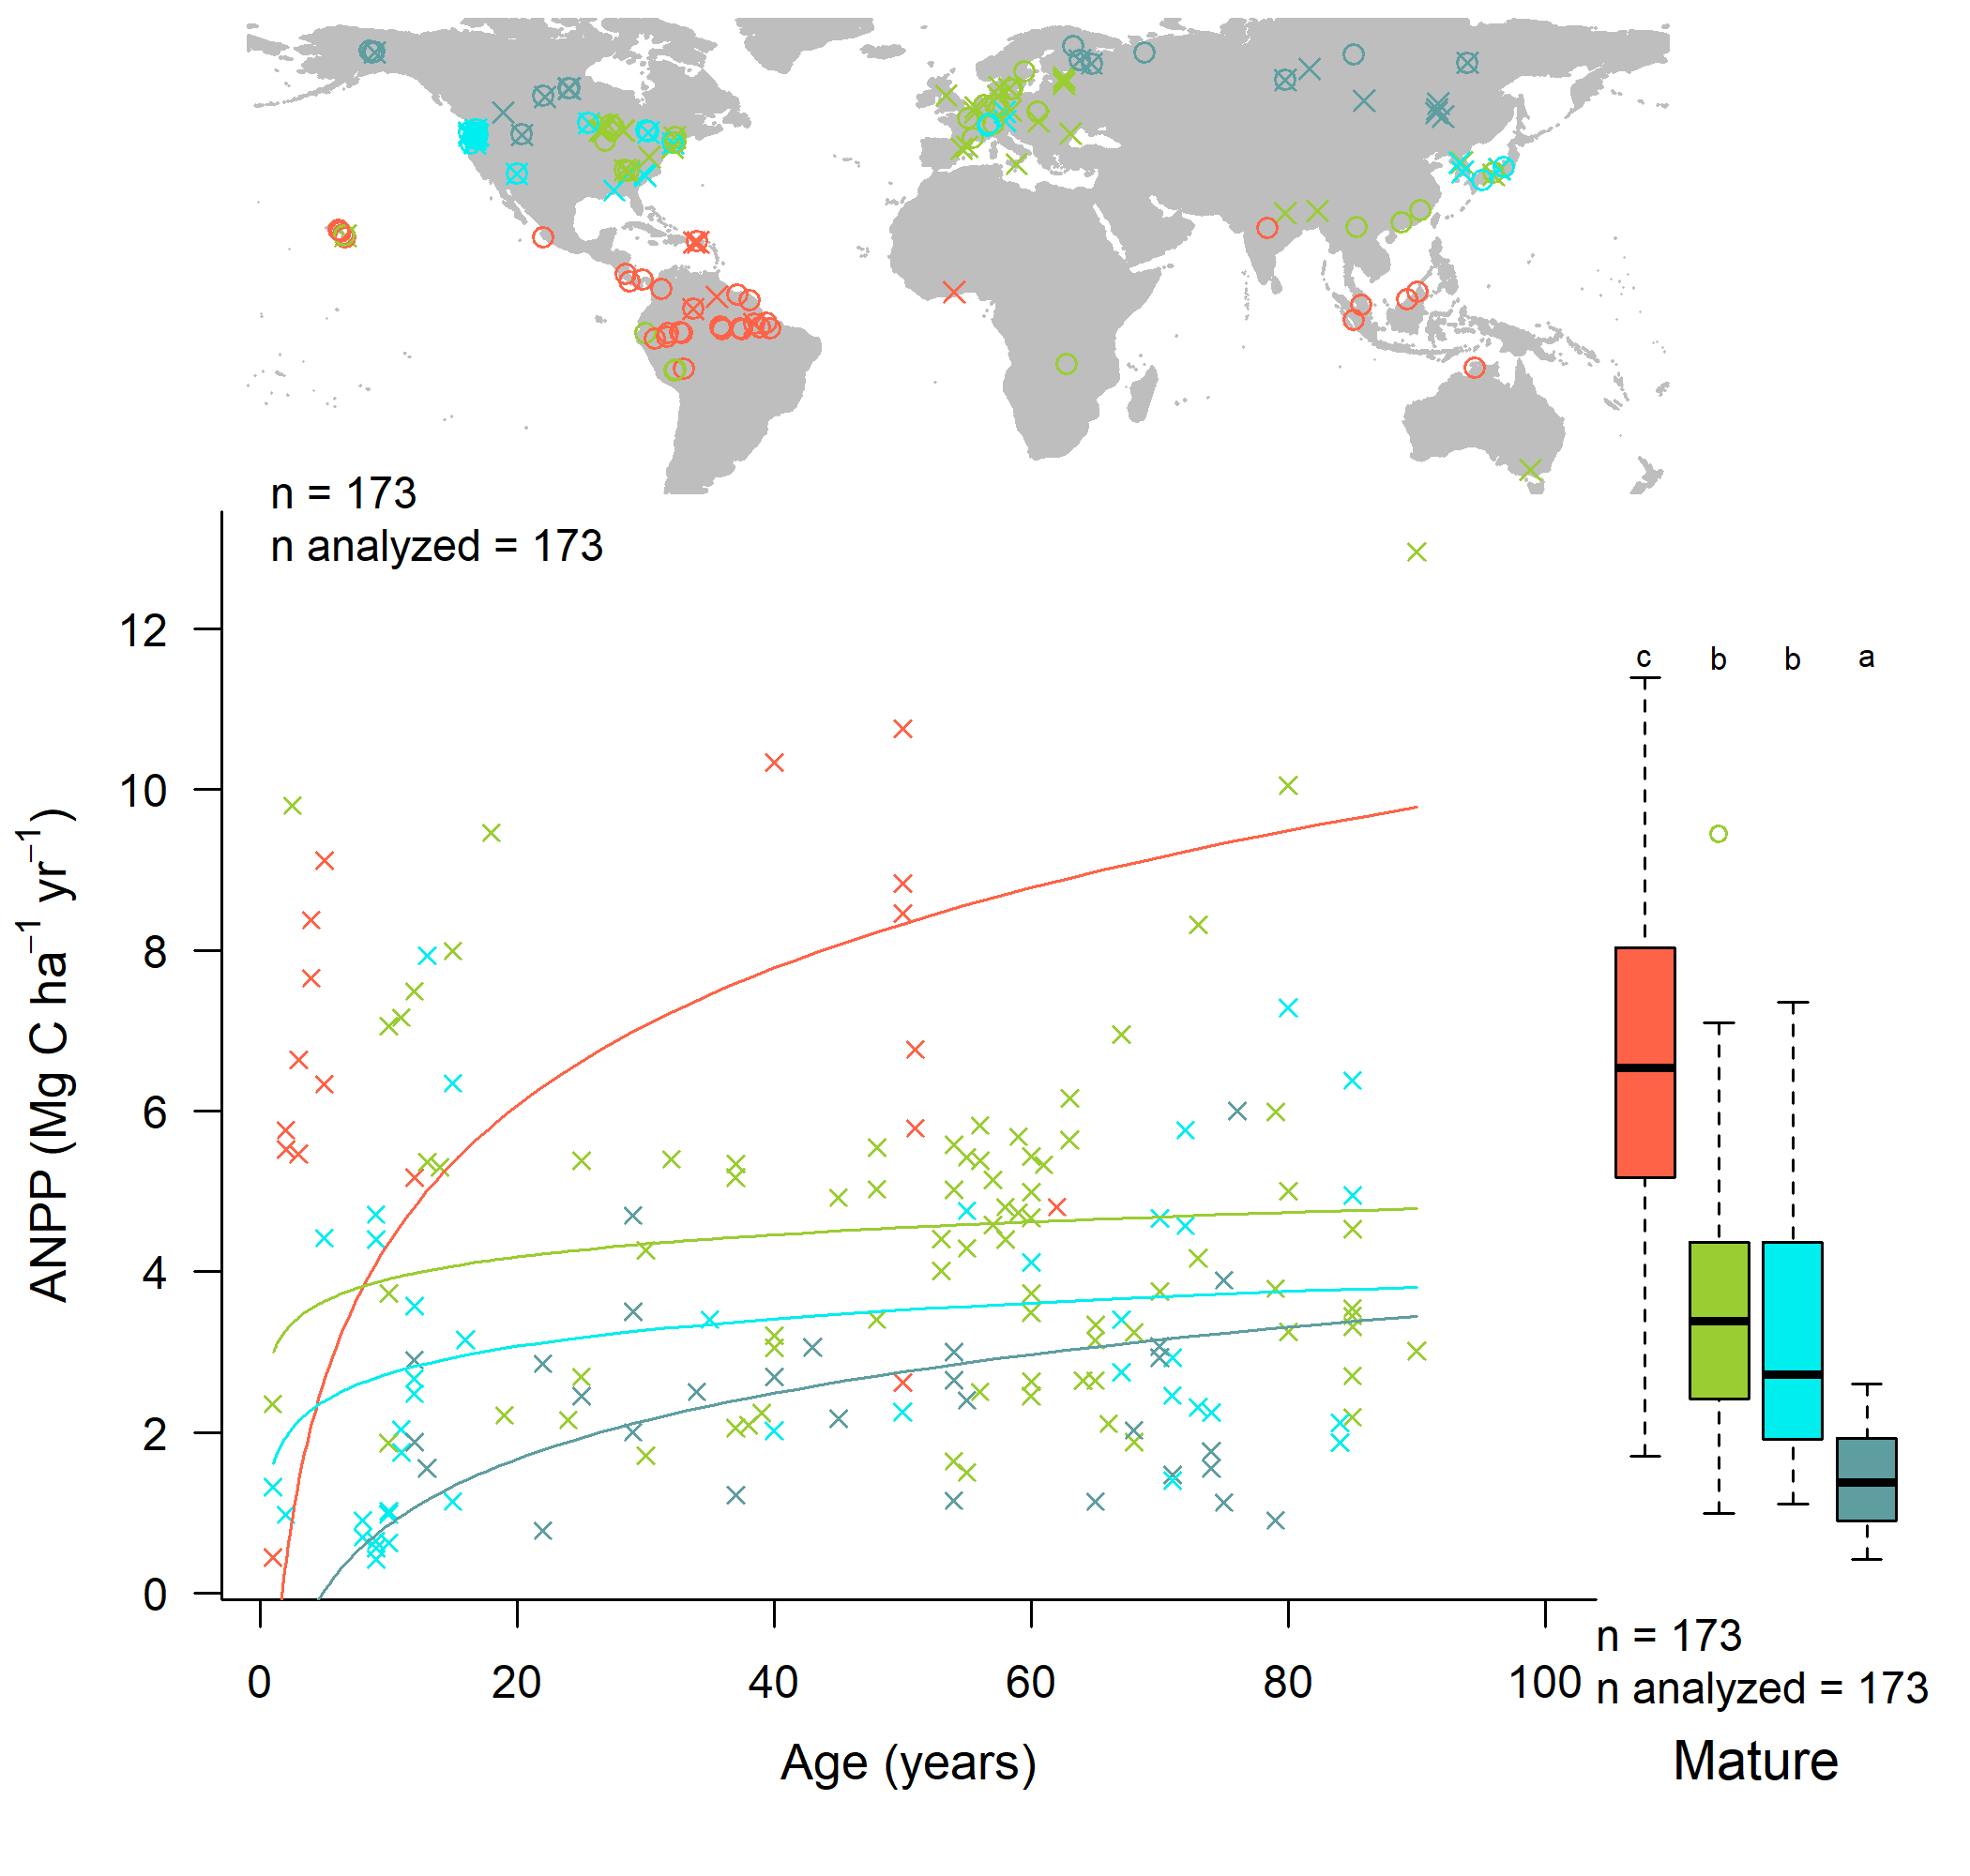
\includegraphics[width=1\linewidth]{tables_figures/age_trends/ANPP_with_map} 

}

\caption{Age trends and biome differences for $ANPP$. Map shows data sources ('$\times$' and '$\circ$' indicate young and mature stands, respectively). In each panel, the left scatterplot shows age trends in forests up to 100 years old, as characterized by a linear mixed effects model with fixed effects of log10(age) and biome. The fitted line indicates the effect of age (solid lines: significant at p<0.05, dashed lines: non-significant), and non-parallel lines indicate a significant log10(age) $\times$ biome interaction. Boxplot illustrates distribution across mature forests, with different letters indicating significant differences between biomes. Data from biomes that did not meet the sample size criteria (see Methods) are plotted, but lack regression lines (young forests) or test of differences across biomes (mature forests).}\label{fig:unnamed-chunk-11}
\end{figure}

\newpage

\hypertarget{figure-s9.-age-trends-and-biome-differences-for-anpp_woody}{%
\subsection{\texorpdfstring{Figure S9. Age trends and biome differences
for
\(ANPP_{woody}\)}{Figure S9. Age trends and biome differences for ANPP\_\{woody\}}}\label{figure-s9.-age-trends-and-biome-differences-for-anpp_woody}}

\begin{figure}[H]

{\centering 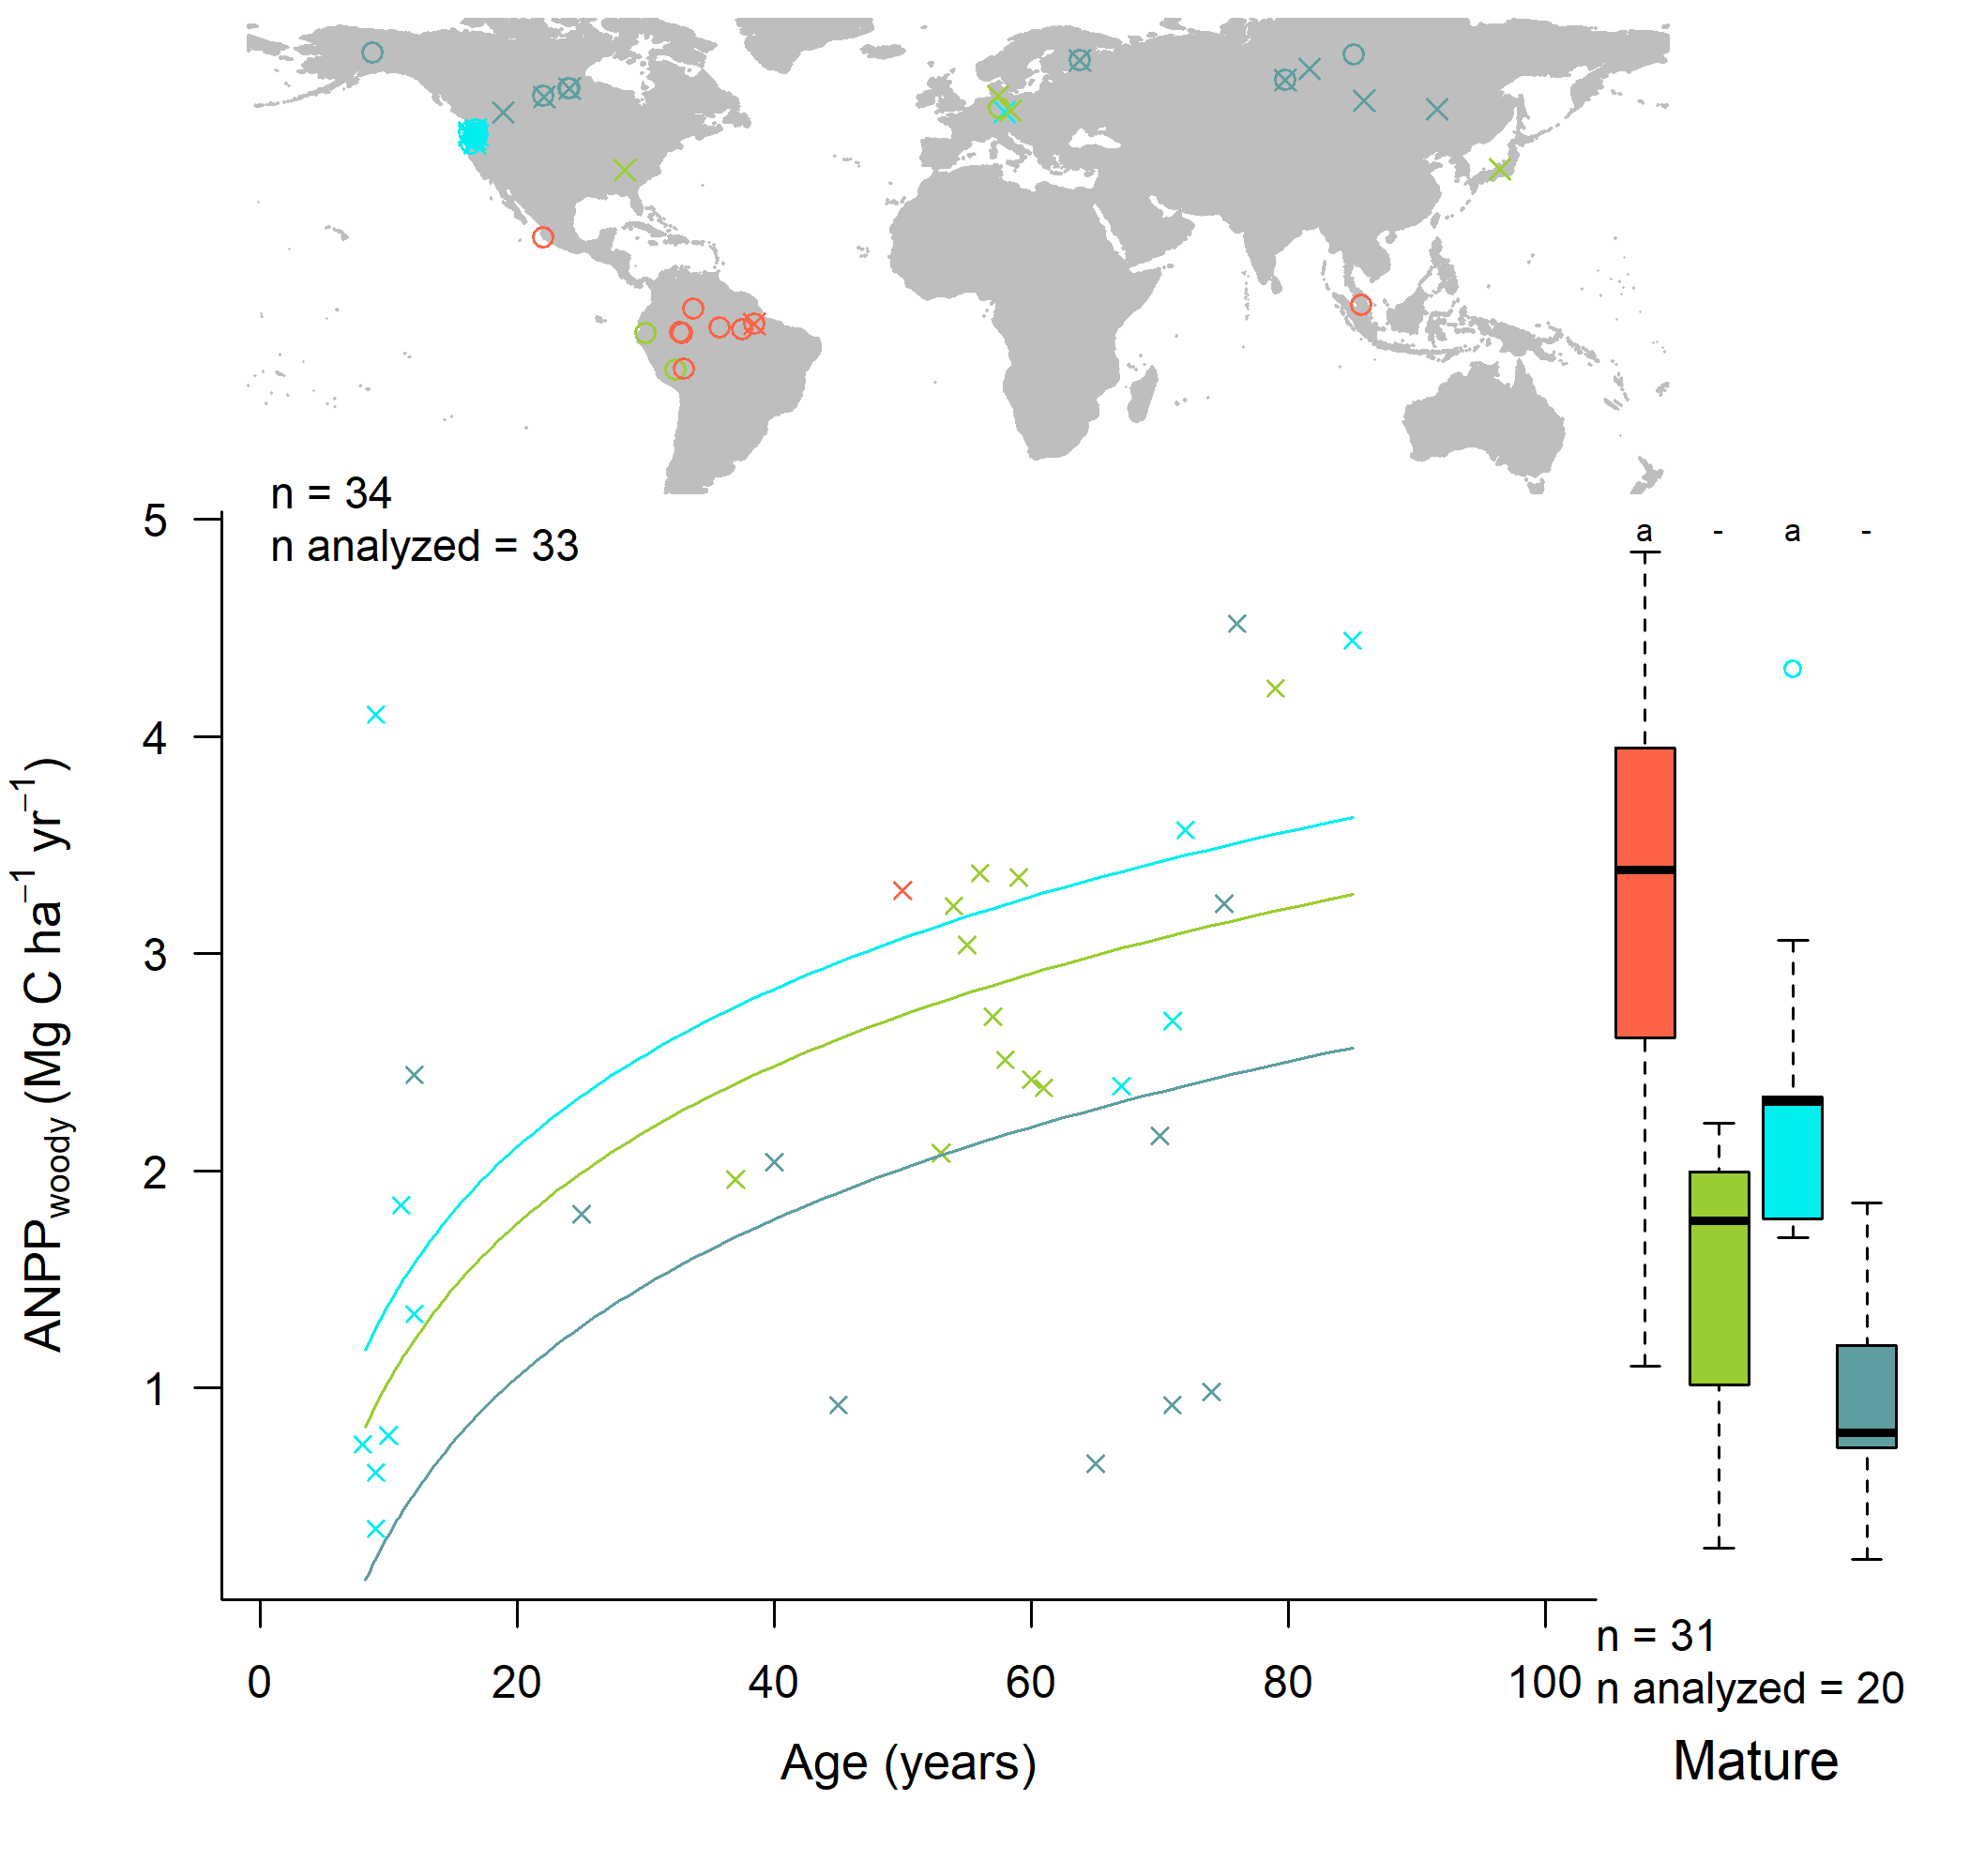
\includegraphics[width=1\linewidth]{tables_figures/age_trends/ANPP_woody_with_map} 

}

\caption{Age trends and biome differences for $ANPP_{woody}$. Map shows data sources ('$\times$' and '$\circ$' indicate young and mature stands, respectively). In each panel, the left scatterplot shows age trends in forests up to 100 years old, as characterized by a linear mixed effects model with fixed effects of log10(age) and biome. The fitted line indicates the effect of age (solid lines: significant at p<0.05, dashed lines: non-significant), and non-parallel lines indicate a significant log10(age) $\times$ biome interaction. Boxplot illustrates distribution across mature forests, with different letters indicating significant differences between biomes. Data from biomes that did not meet the sample size criteria (see Methods) are plotted, but lack regression lines (young forests) or test of differences across biomes (mature forests).}\label{fig:unnamed-chunk-12}
\end{figure}

\newpage

\hypertarget{figure-s10.-age-trends-and-biome-differences-for-anpp_stem}{%
\subsection{\texorpdfstring{Figure S10. Age trends and biome differences
for
\(ANPP_{stem}\)}{Figure S10. Age trends and biome differences for ANPP\_\{stem\}}}\label{figure-s10.-age-trends-and-biome-differences-for-anpp_stem}}

\begin{figure}[H]

{\centering 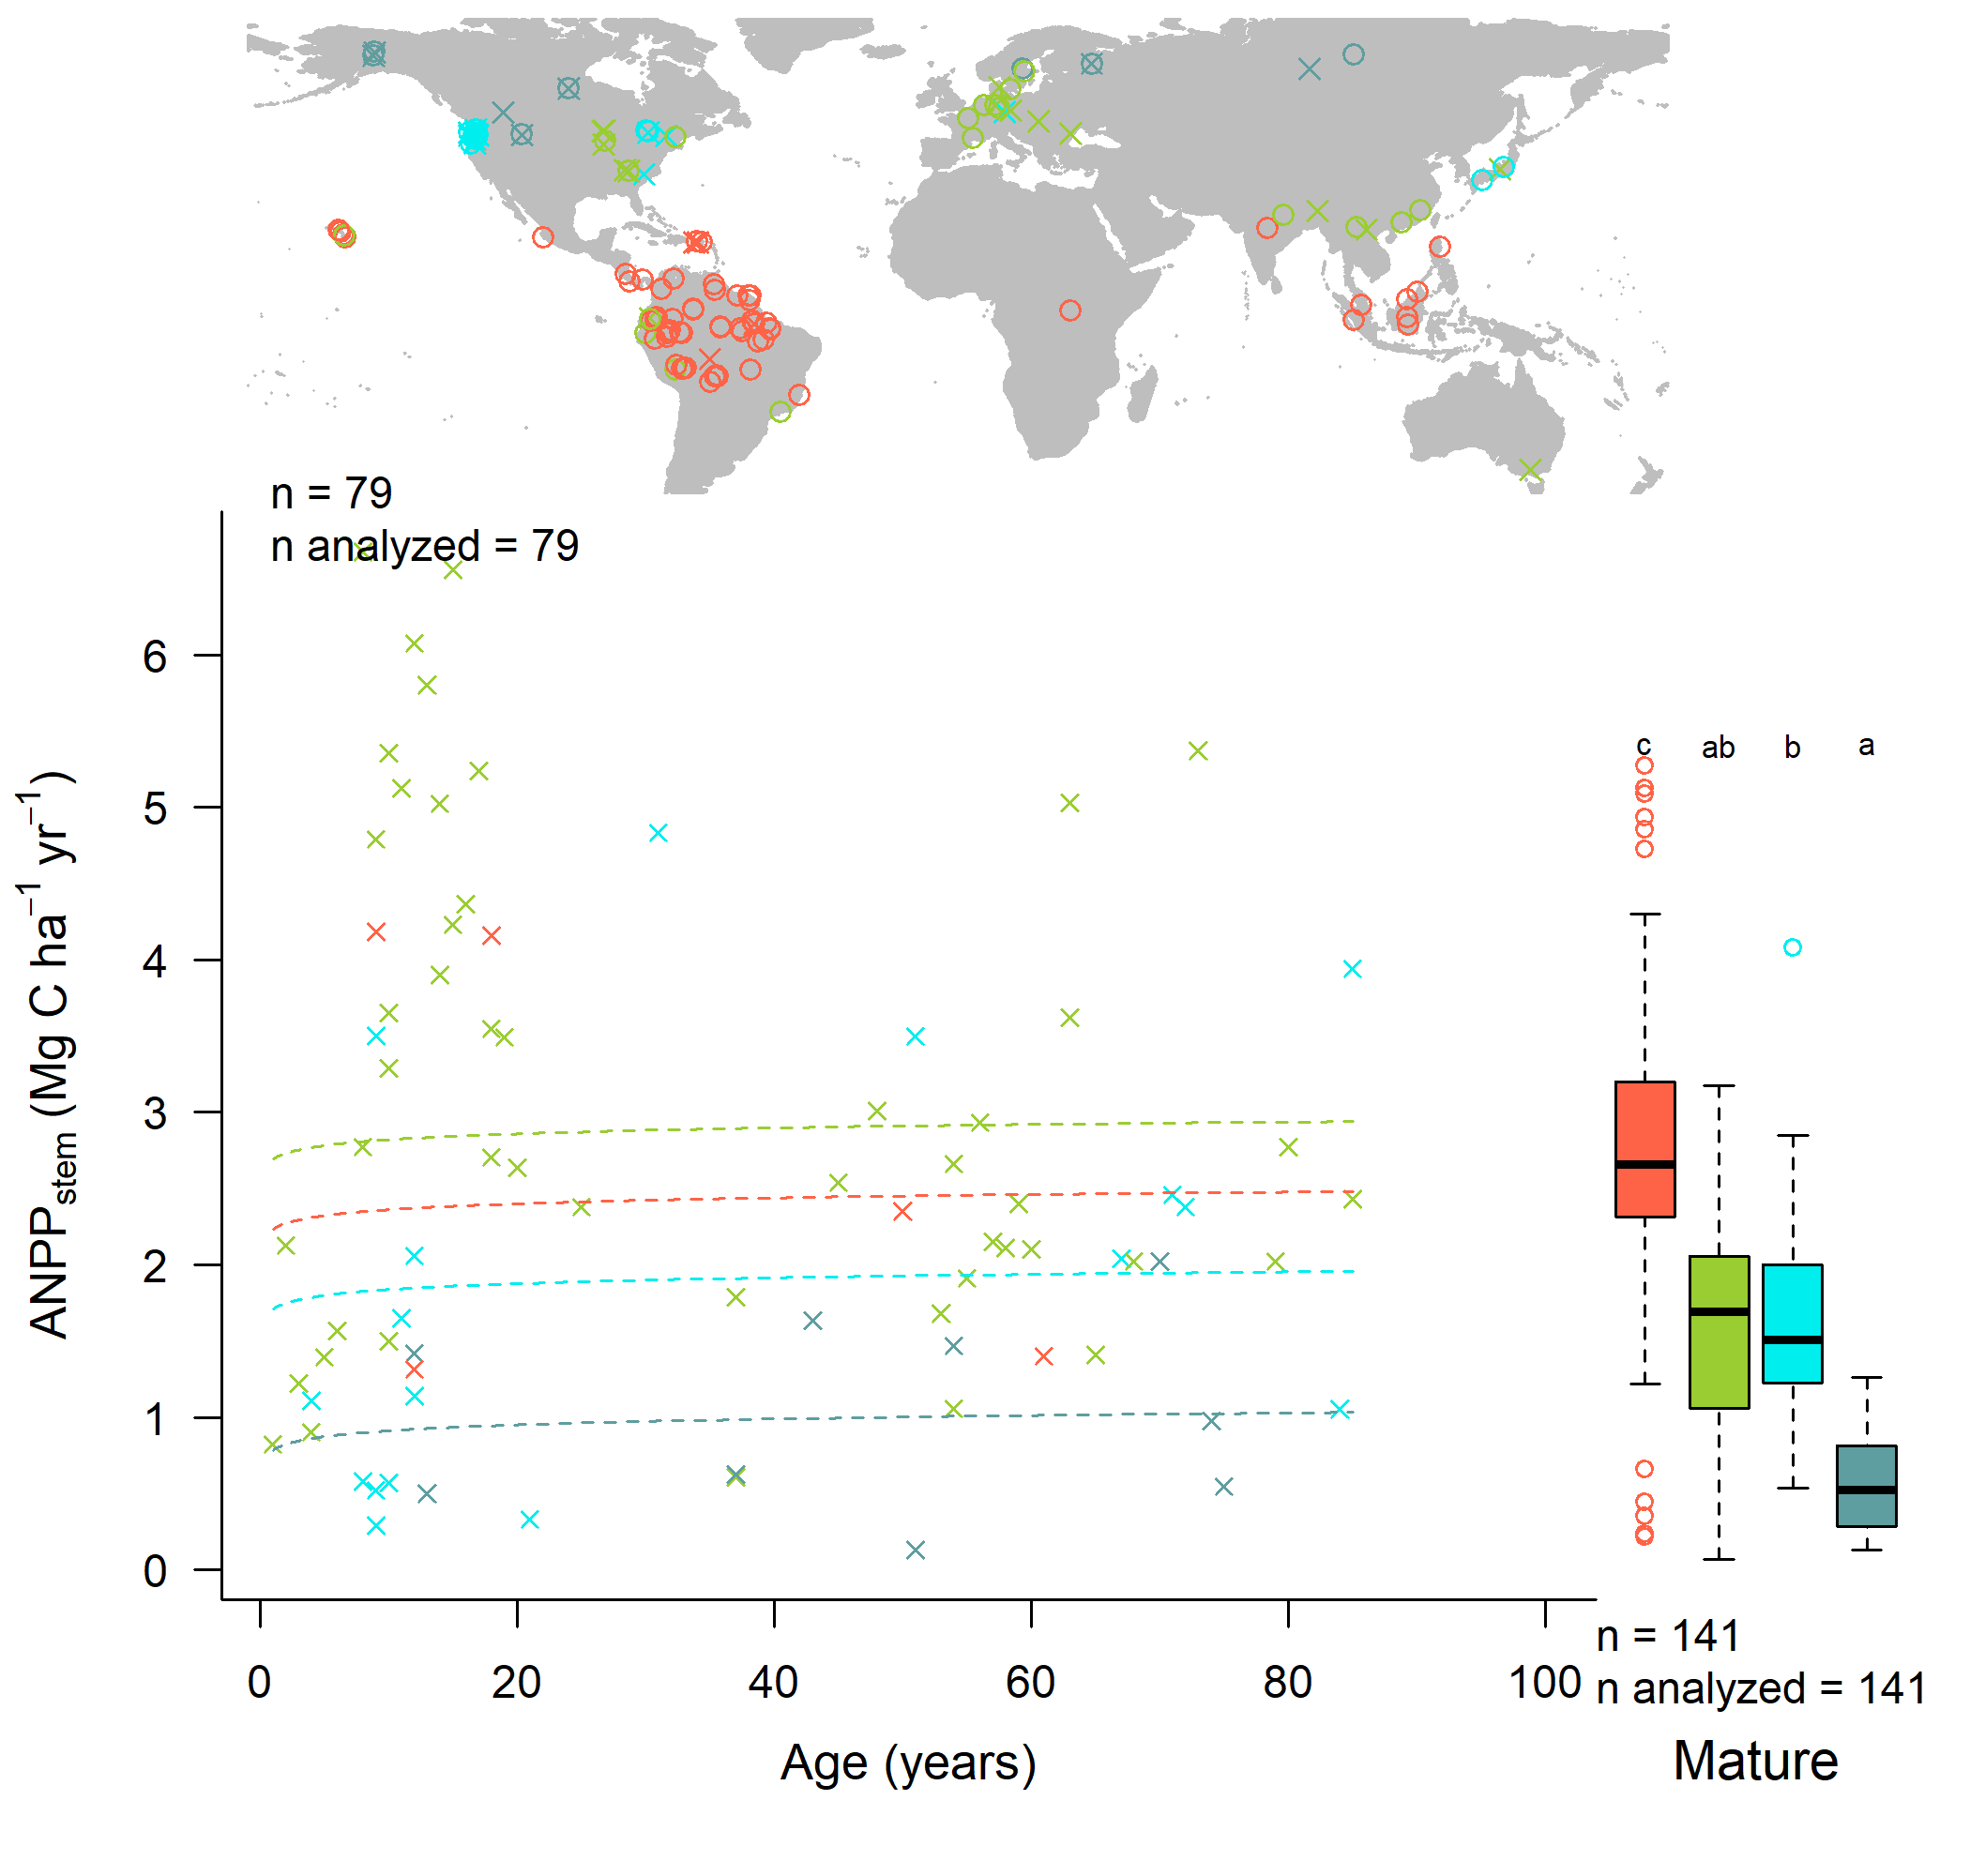
\includegraphics[width=1\linewidth]{tables_figures/age_trends/ANPP_stem_with_map} 

}

\caption{Age trends and biome differences for $ANPP_{stem}$. Map shows data sources ('$\times$' and '$\circ$' indicate young and mature stands, respectively). In each panel, the left scatterplot shows age trends in forests up to 100 years old, as characterized by a linear mixed effects model with fixed effects of log10(age) and biome. The fitted line indicates the effect of age (solid lines: significant at p<0.05, dashed lines: non-significant), and non-parallel lines indicate a significant log10(age) $\times$ biome interaction. Boxplot illustrates distribution across mature forests, with different letters indicating significant differences between biomes. Data from biomes that did not meet the sample size criteria (see Methods) are plotted, but lack regression lines (young forests) or test of differences across biomes (mature forests).}\label{fig:unnamed-chunk-13}
\end{figure}

\newpage

\hypertarget{figure-s11.-age-trends-and-biome-differences-for-anpp_foliage}{%
\subsection{\texorpdfstring{Figure S11. Age trends and biome differences
for
\(ANPP_{foliage}\)}{Figure S11. Age trends and biome differences for ANPP\_\{foliage\}}}\label{figure-s11.-age-trends-and-biome-differences-for-anpp_foliage}}

\begin{figure}[H]

{\centering 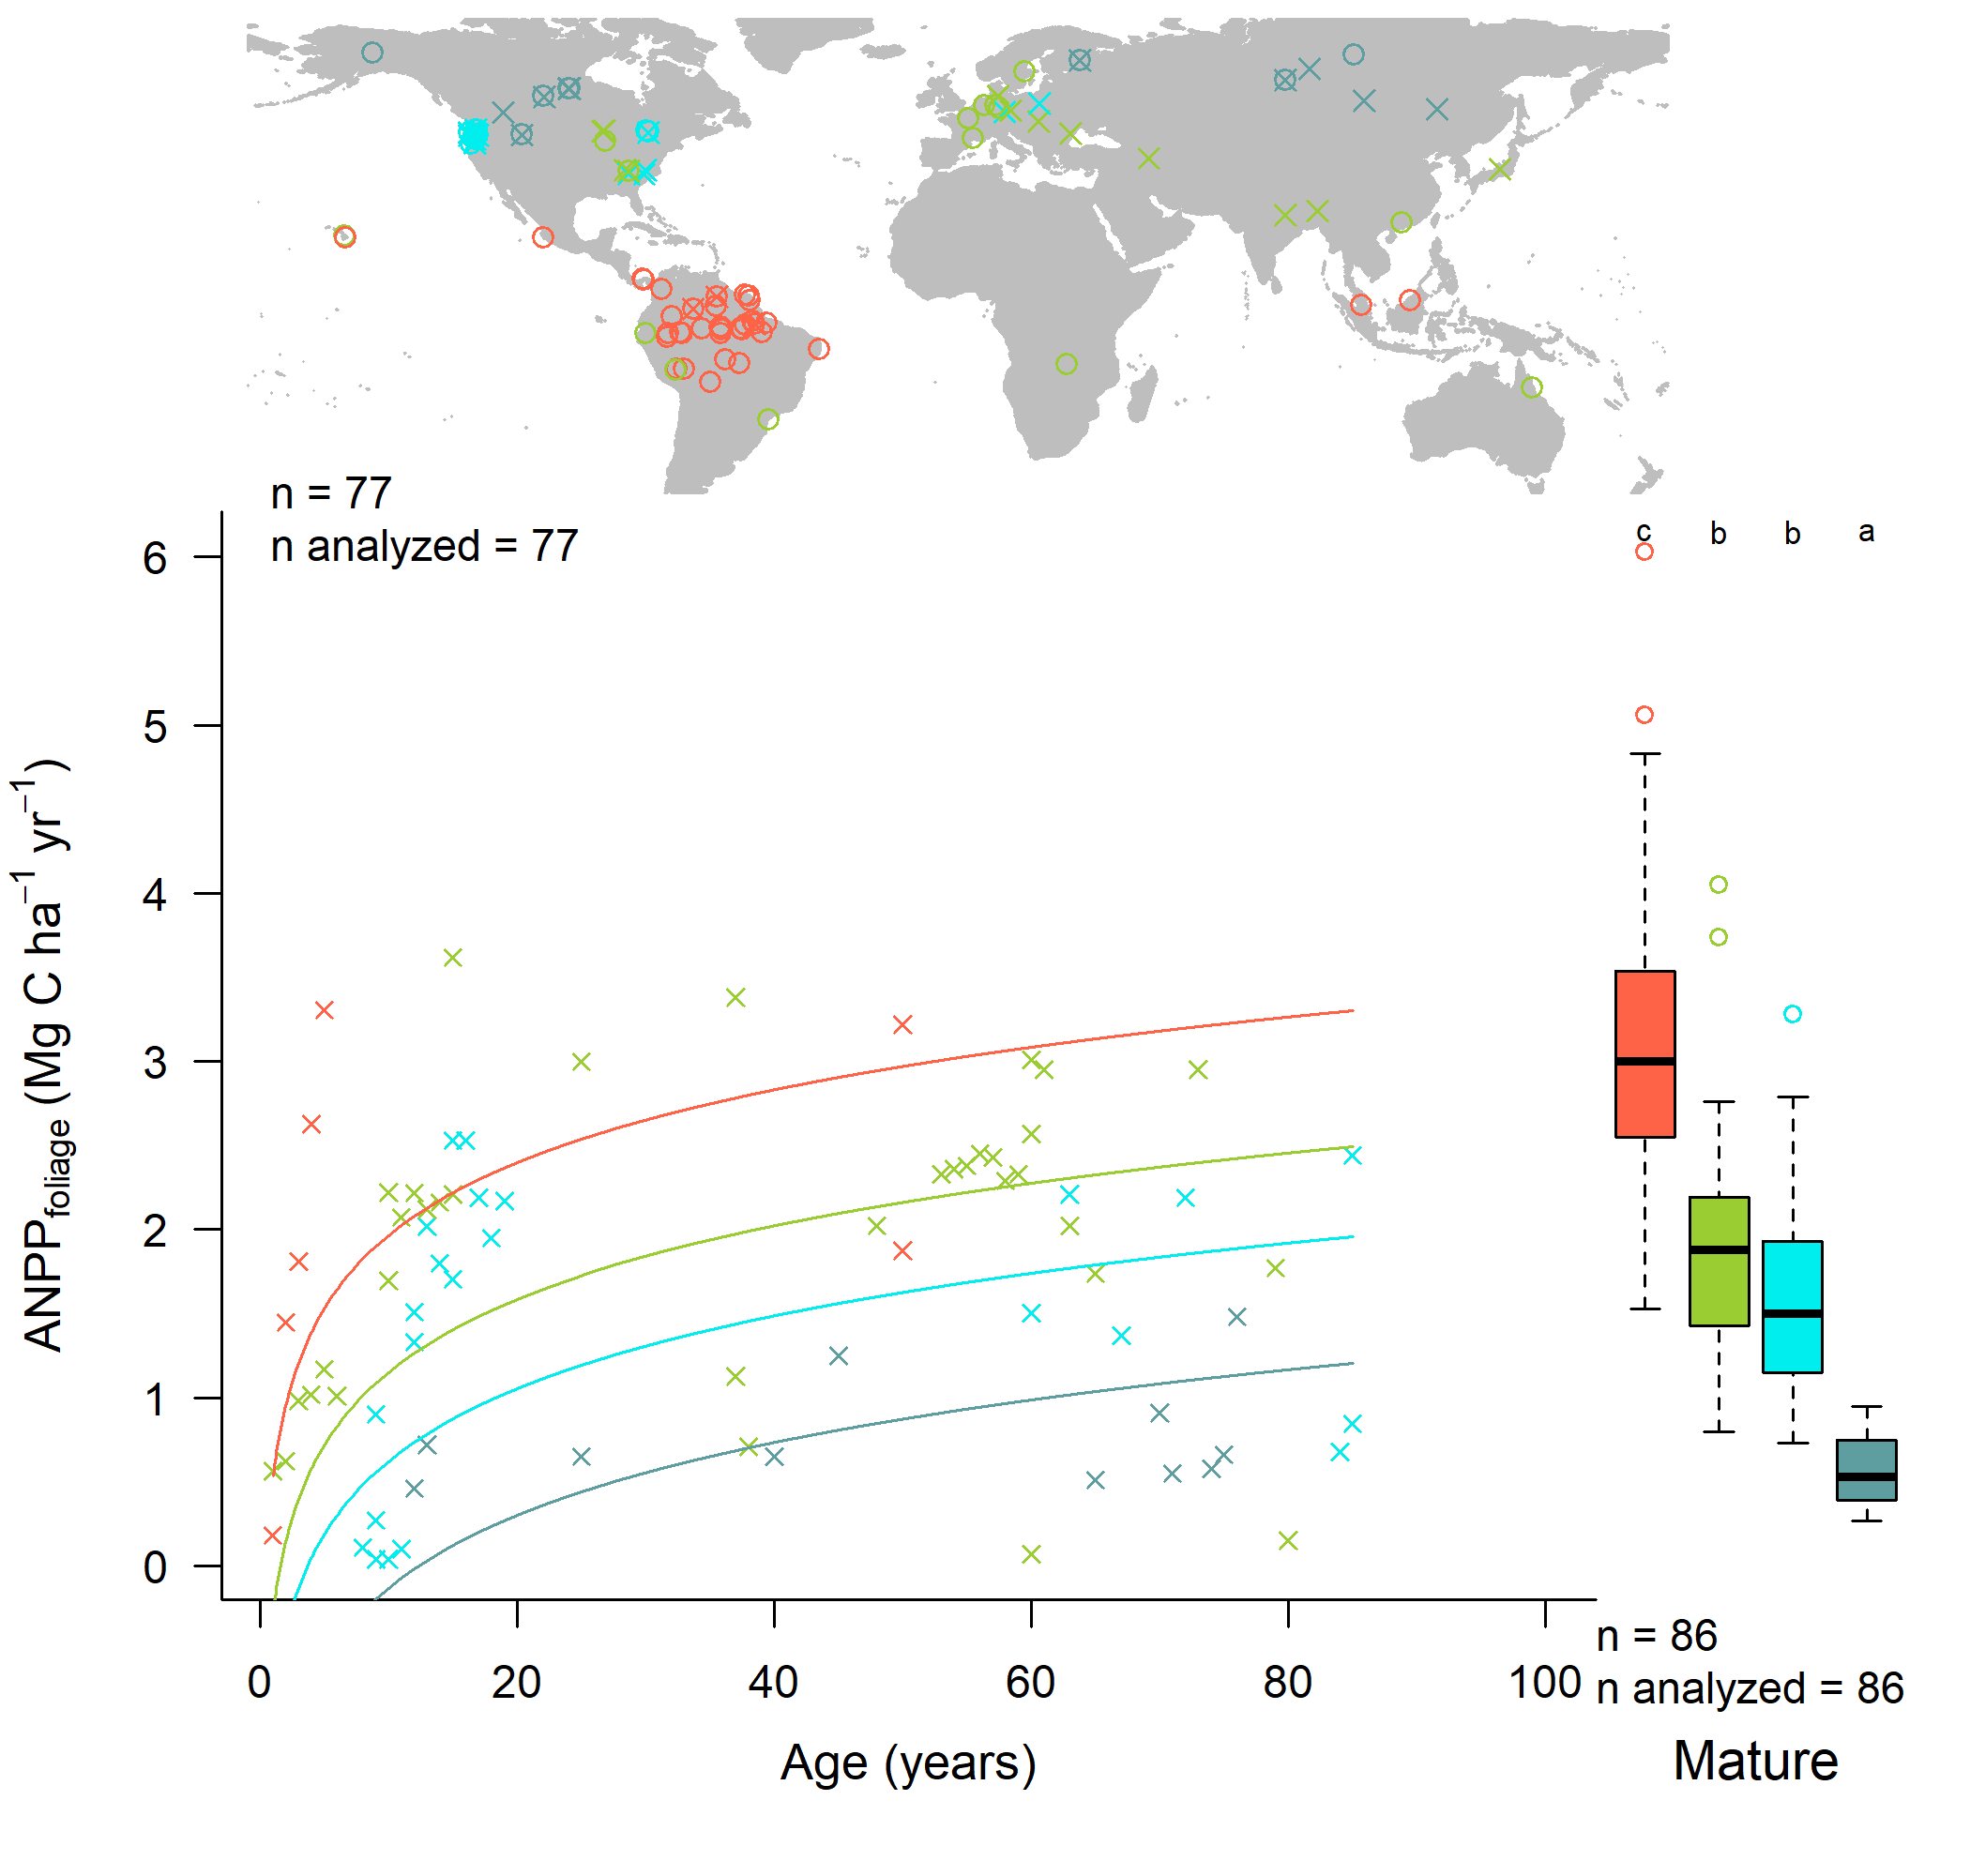
\includegraphics[width=1\linewidth]{tables_figures/age_trends/ANPP_foliage_with_map} 

}

\caption{Age trends and biome differences for $ANPP_{foliage}$. Map shows data sources ('$\times$' and '$\circ$' indicate young and mature stands, respectively). In each panel, the left scatterplot shows age trends in forests up to 100 years old, as characterized by a linear mixed effects model with fixed effects of log10(age) and biome. The fitted line indicates the effect of age (solid lines: significant at p<0.05, dashed lines: non-significant), and non-parallel lines indicate a significant log10(age) $\times$ biome interaction. Boxplot illustrates distribution across mature forests, with different letters indicating significant differences between biomes. Data from biomes that did not meet the sample size criteria (see Methods) are plotted, but lack regression lines (young forests) or test of differences across biomes (mature forests).}\label{fig:unnamed-chunk-14}
\end{figure}

\newpage

\hypertarget{figure-s12.-age-trends-and-biome-differences-for-anpp_litterfall}{%
\subsection{\texorpdfstring{Figure S12. Age trends and biome differences
for
\(ANPP_{litterfall}\)}{Figure S12. Age trends and biome differences for ANPP\_\{litterfall\}}}\label{figure-s12.-age-trends-and-biome-differences-for-anpp_litterfall}}

\begin{figure}[H]

{\centering 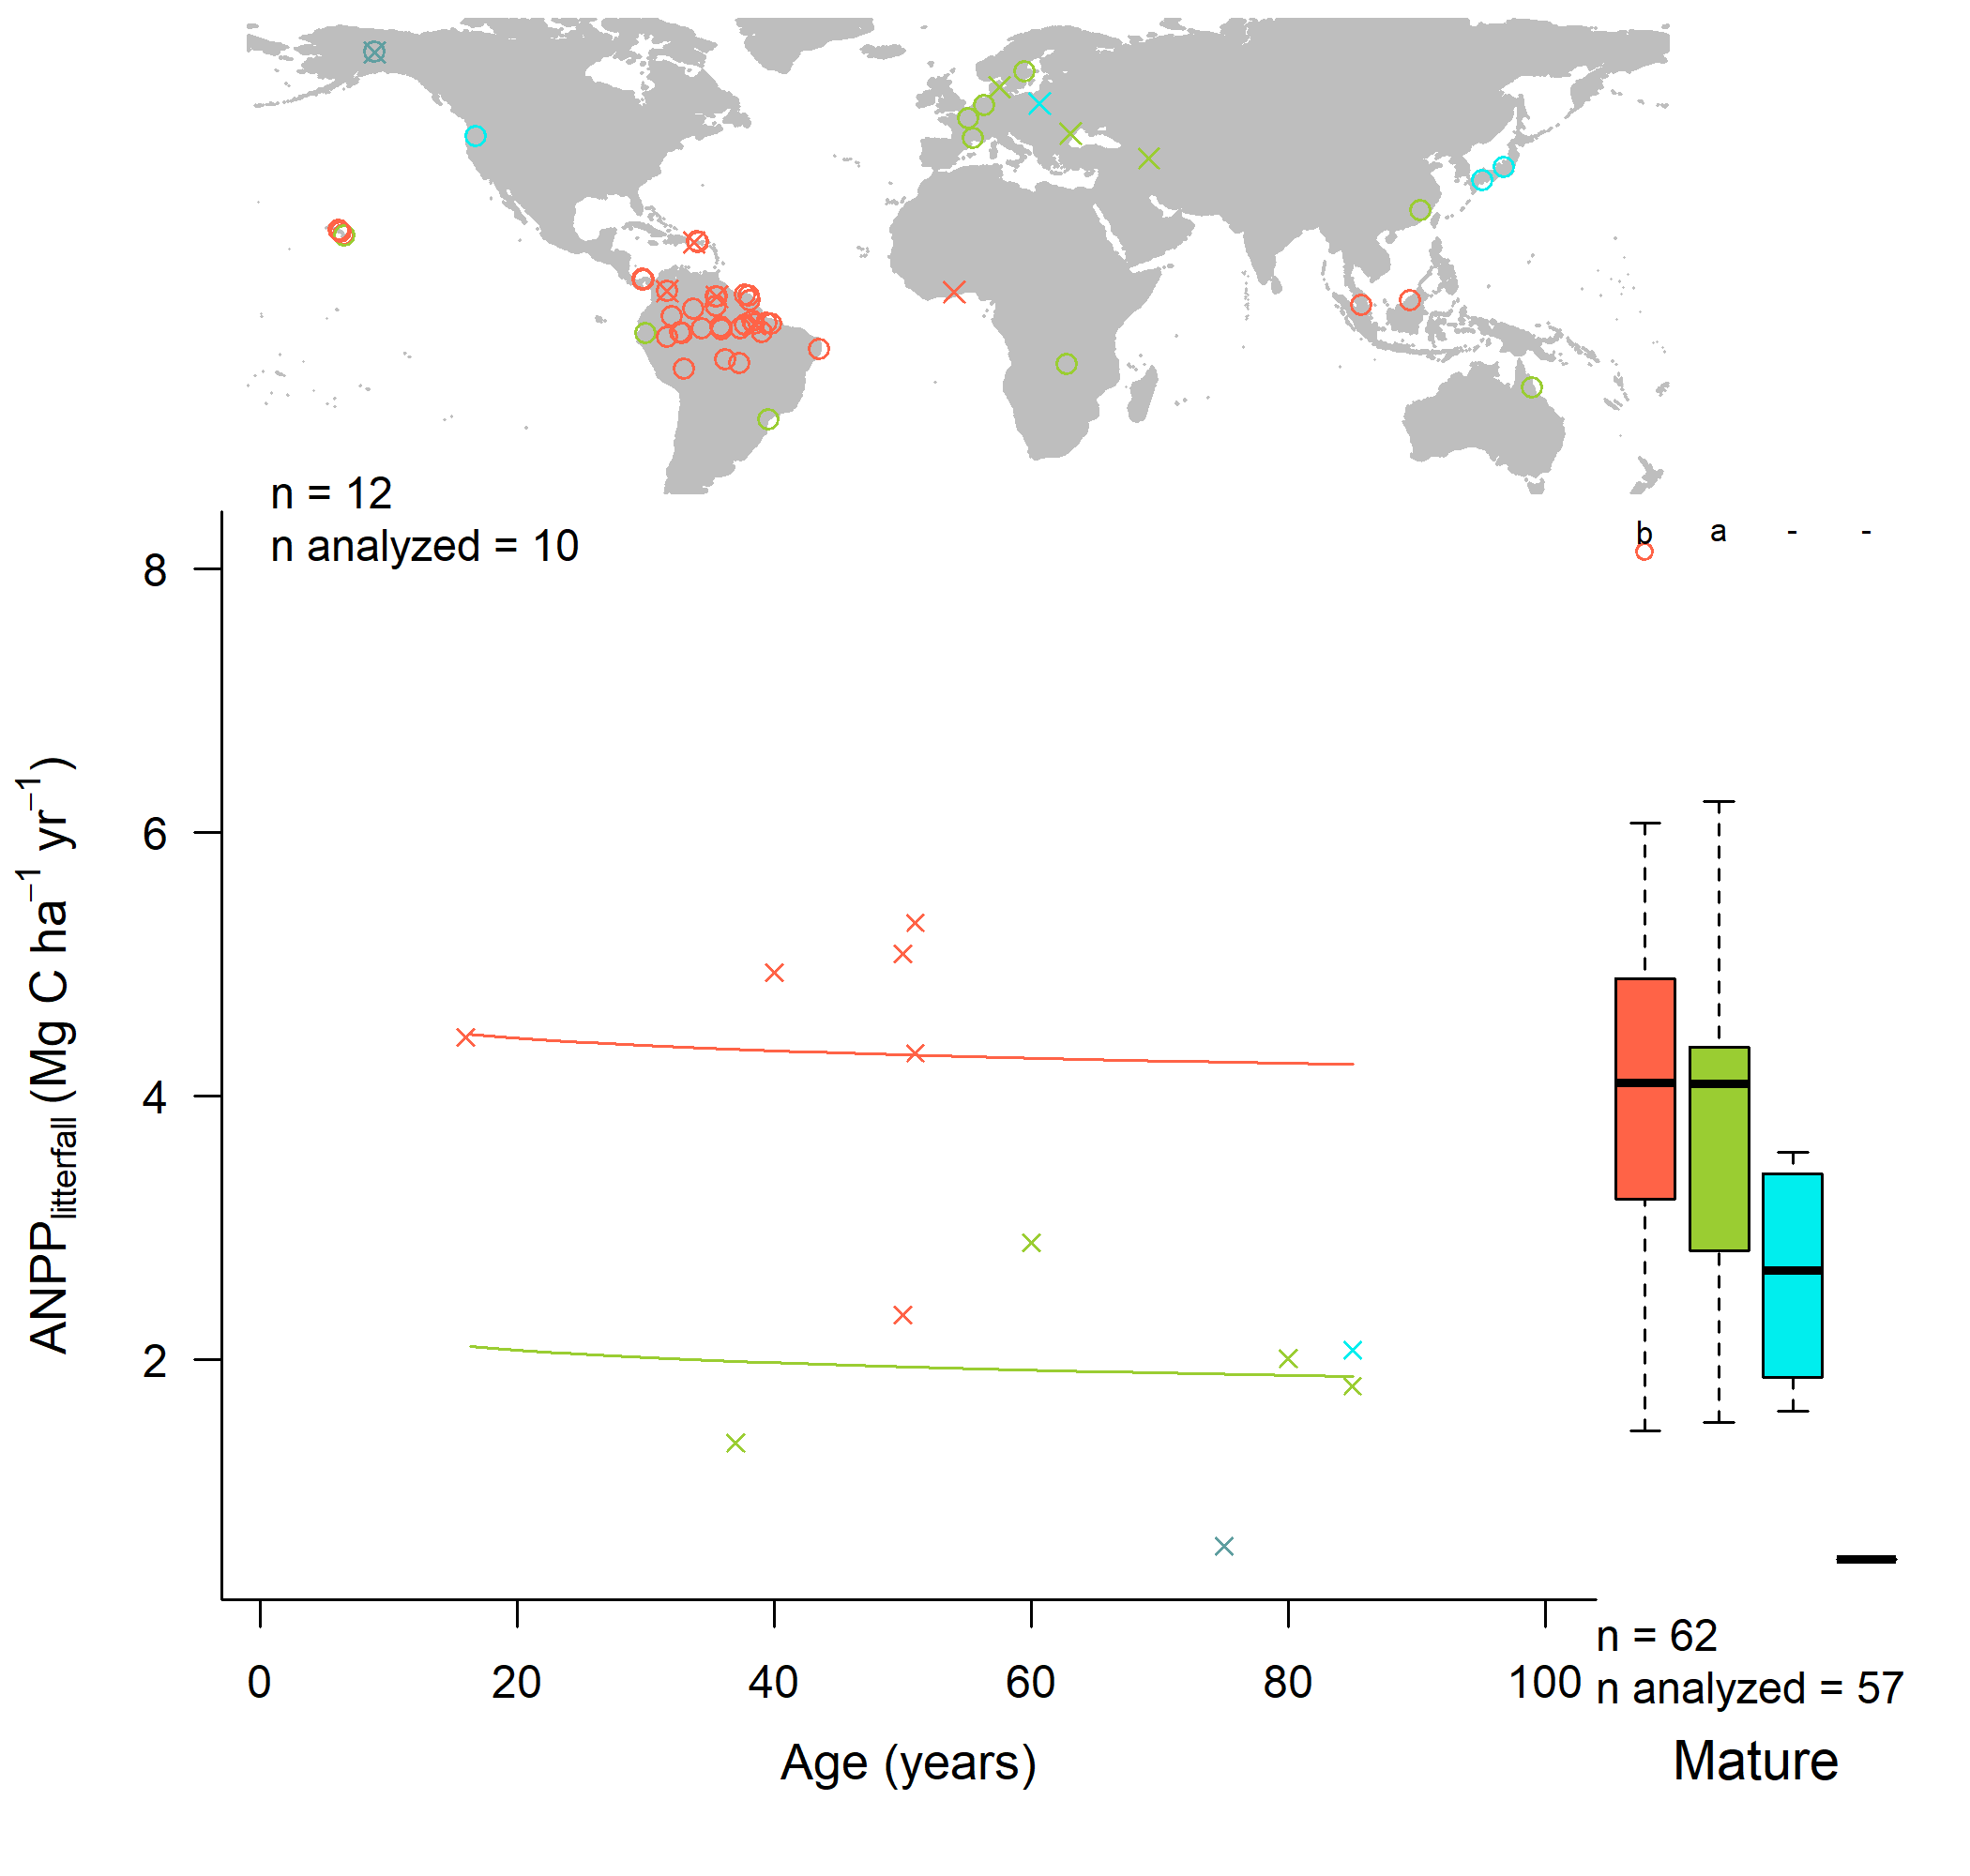
\includegraphics[width=1\linewidth]{tables_figures/age_trends/ANPP_litterfall_with_map} 

}

\caption{Age trends and biome differences for $ANPP_{litterfall}$. Map shows data sources ('$\times$' and '$\circ$' indicate young and mature stands, respectively). In each panel, the left scatterplot shows age trends in forests up to 100 years old, as characterized by a linear mixed effects model with fixed effects of log10(age) and biome. The fitted line indicates the effect of age (solid lines: significant at p<0.05, dashed lines: non-significant), and non-parallel lines indicate a significant log10(age) $\times$ biome interaction. Boxplot illustrates distribution across mature forests, with different letters indicating significant differences between biomes. Data from biomes that did not meet the sample size criteria (see Methods) are plotted, but lack regression lines (young forests) or test of differences across biomes (mature forests).}\label{fig:unnamed-chunk-15}
\end{figure}

\newpage

\hypertarget{figure-s13.-age-trends-and-biome-differences-for-bnpp}{%
\subsection{\texorpdfstring{Figure S13. Age trends and biome differences
for
\(BNPP\)}{Figure S13. Age trends and biome differences for BNPP}}\label{figure-s13.-age-trends-and-biome-differences-for-bnpp}}

\begin{figure}[H]

{\centering 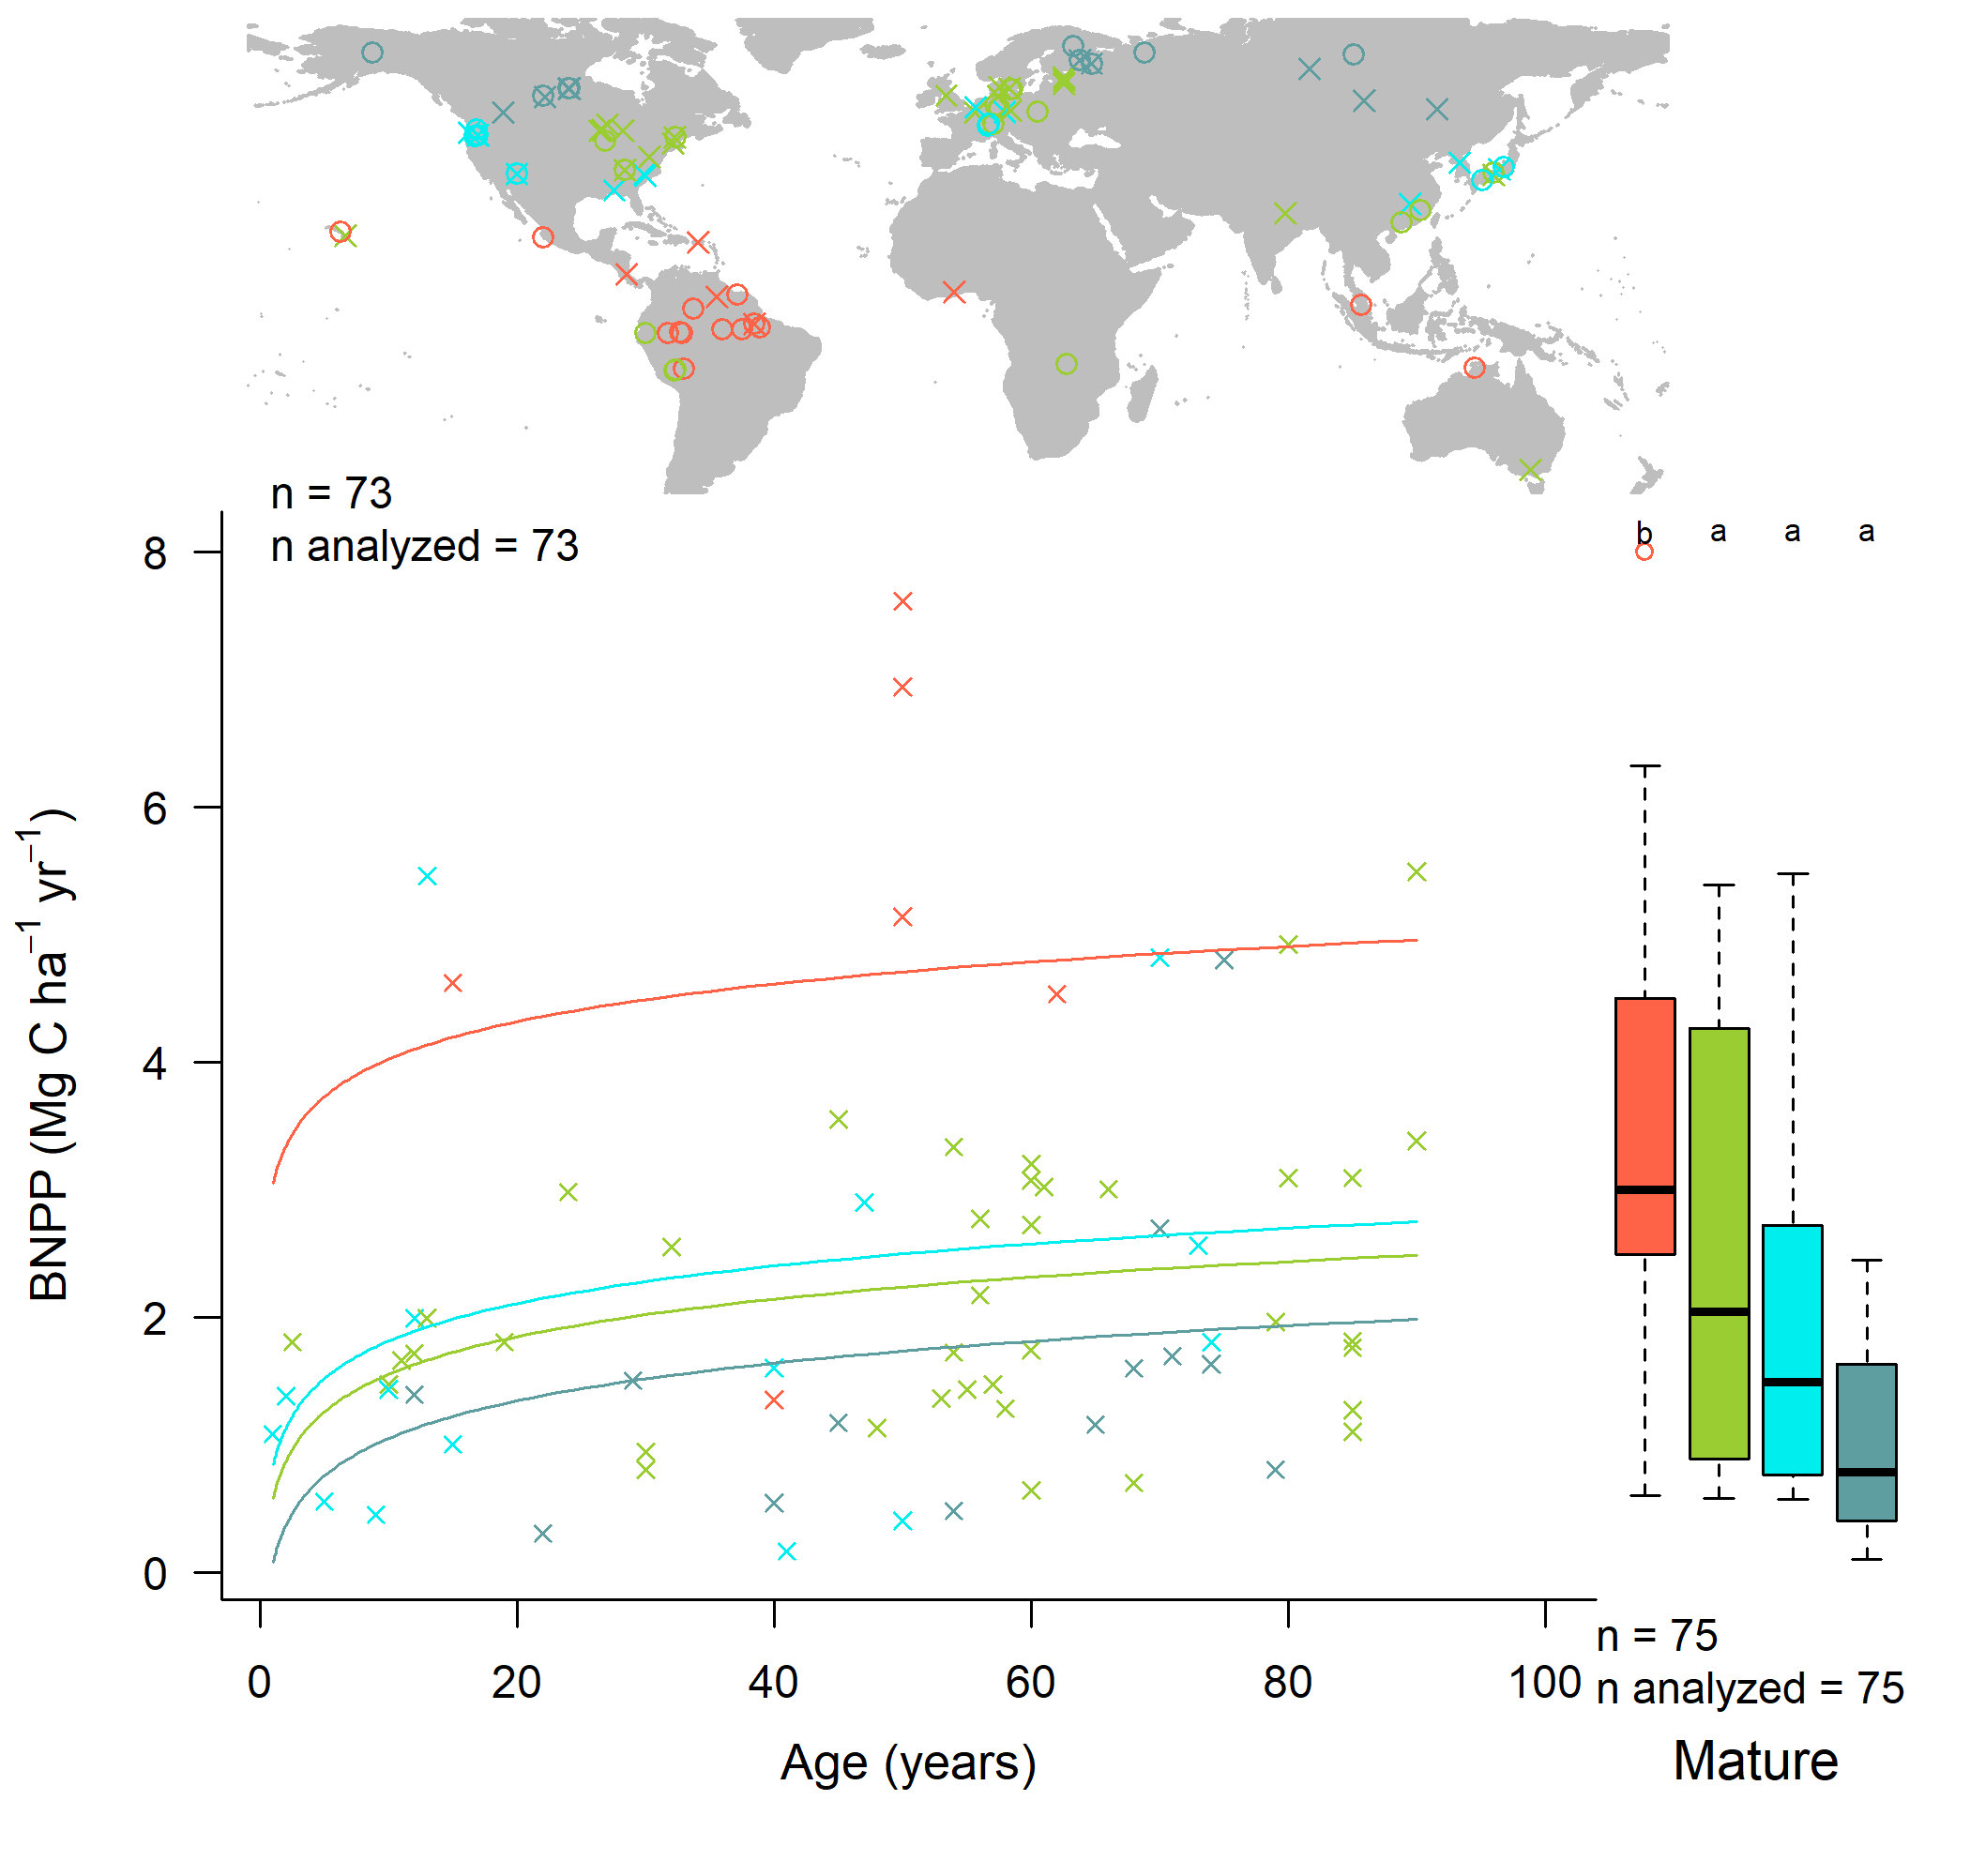
\includegraphics[width=1\linewidth]{tables_figures/age_trends/BNPP_with_map} 

}

\caption{Age trends and biome differences for $BNPP$. Map shows data sources ('$\times$' and '$\circ$' indicate young and mature stands, respectively). In each panel, the left scatterplot shows age trends in forests up to 100 years old, as characterized by a linear mixed effects model with fixed effects of log10(age) and biome. The fitted line indicates the effect of age (solid lines: significant at p<0.05, dashed lines: non-significant), and non-parallel lines indicate a significant log10(age) $\times$ biome interaction. Boxplot illustrates distribution across mature forests, with different letters indicating significant differences between biomes. Data from biomes that did not meet the sample size criteria (see Methods) are plotted, but lack regression lines (young forests) or test of differences across biomes (mature forests).}\label{fig:unnamed-chunk-16}
\end{figure}

\newpage

\hypertarget{figure-s14.-age-trends-and-biome-differences-for-bnpp_coarse}{%
\subsection{\texorpdfstring{Figure S14. Age trends and biome differences
for
\(BNPP_{coarse}\)}{Figure S14. Age trends and biome differences for BNPP\_\{coarse\}}}\label{figure-s14.-age-trends-and-biome-differences-for-bnpp_coarse}}

\begin{figure}[H]

{\centering 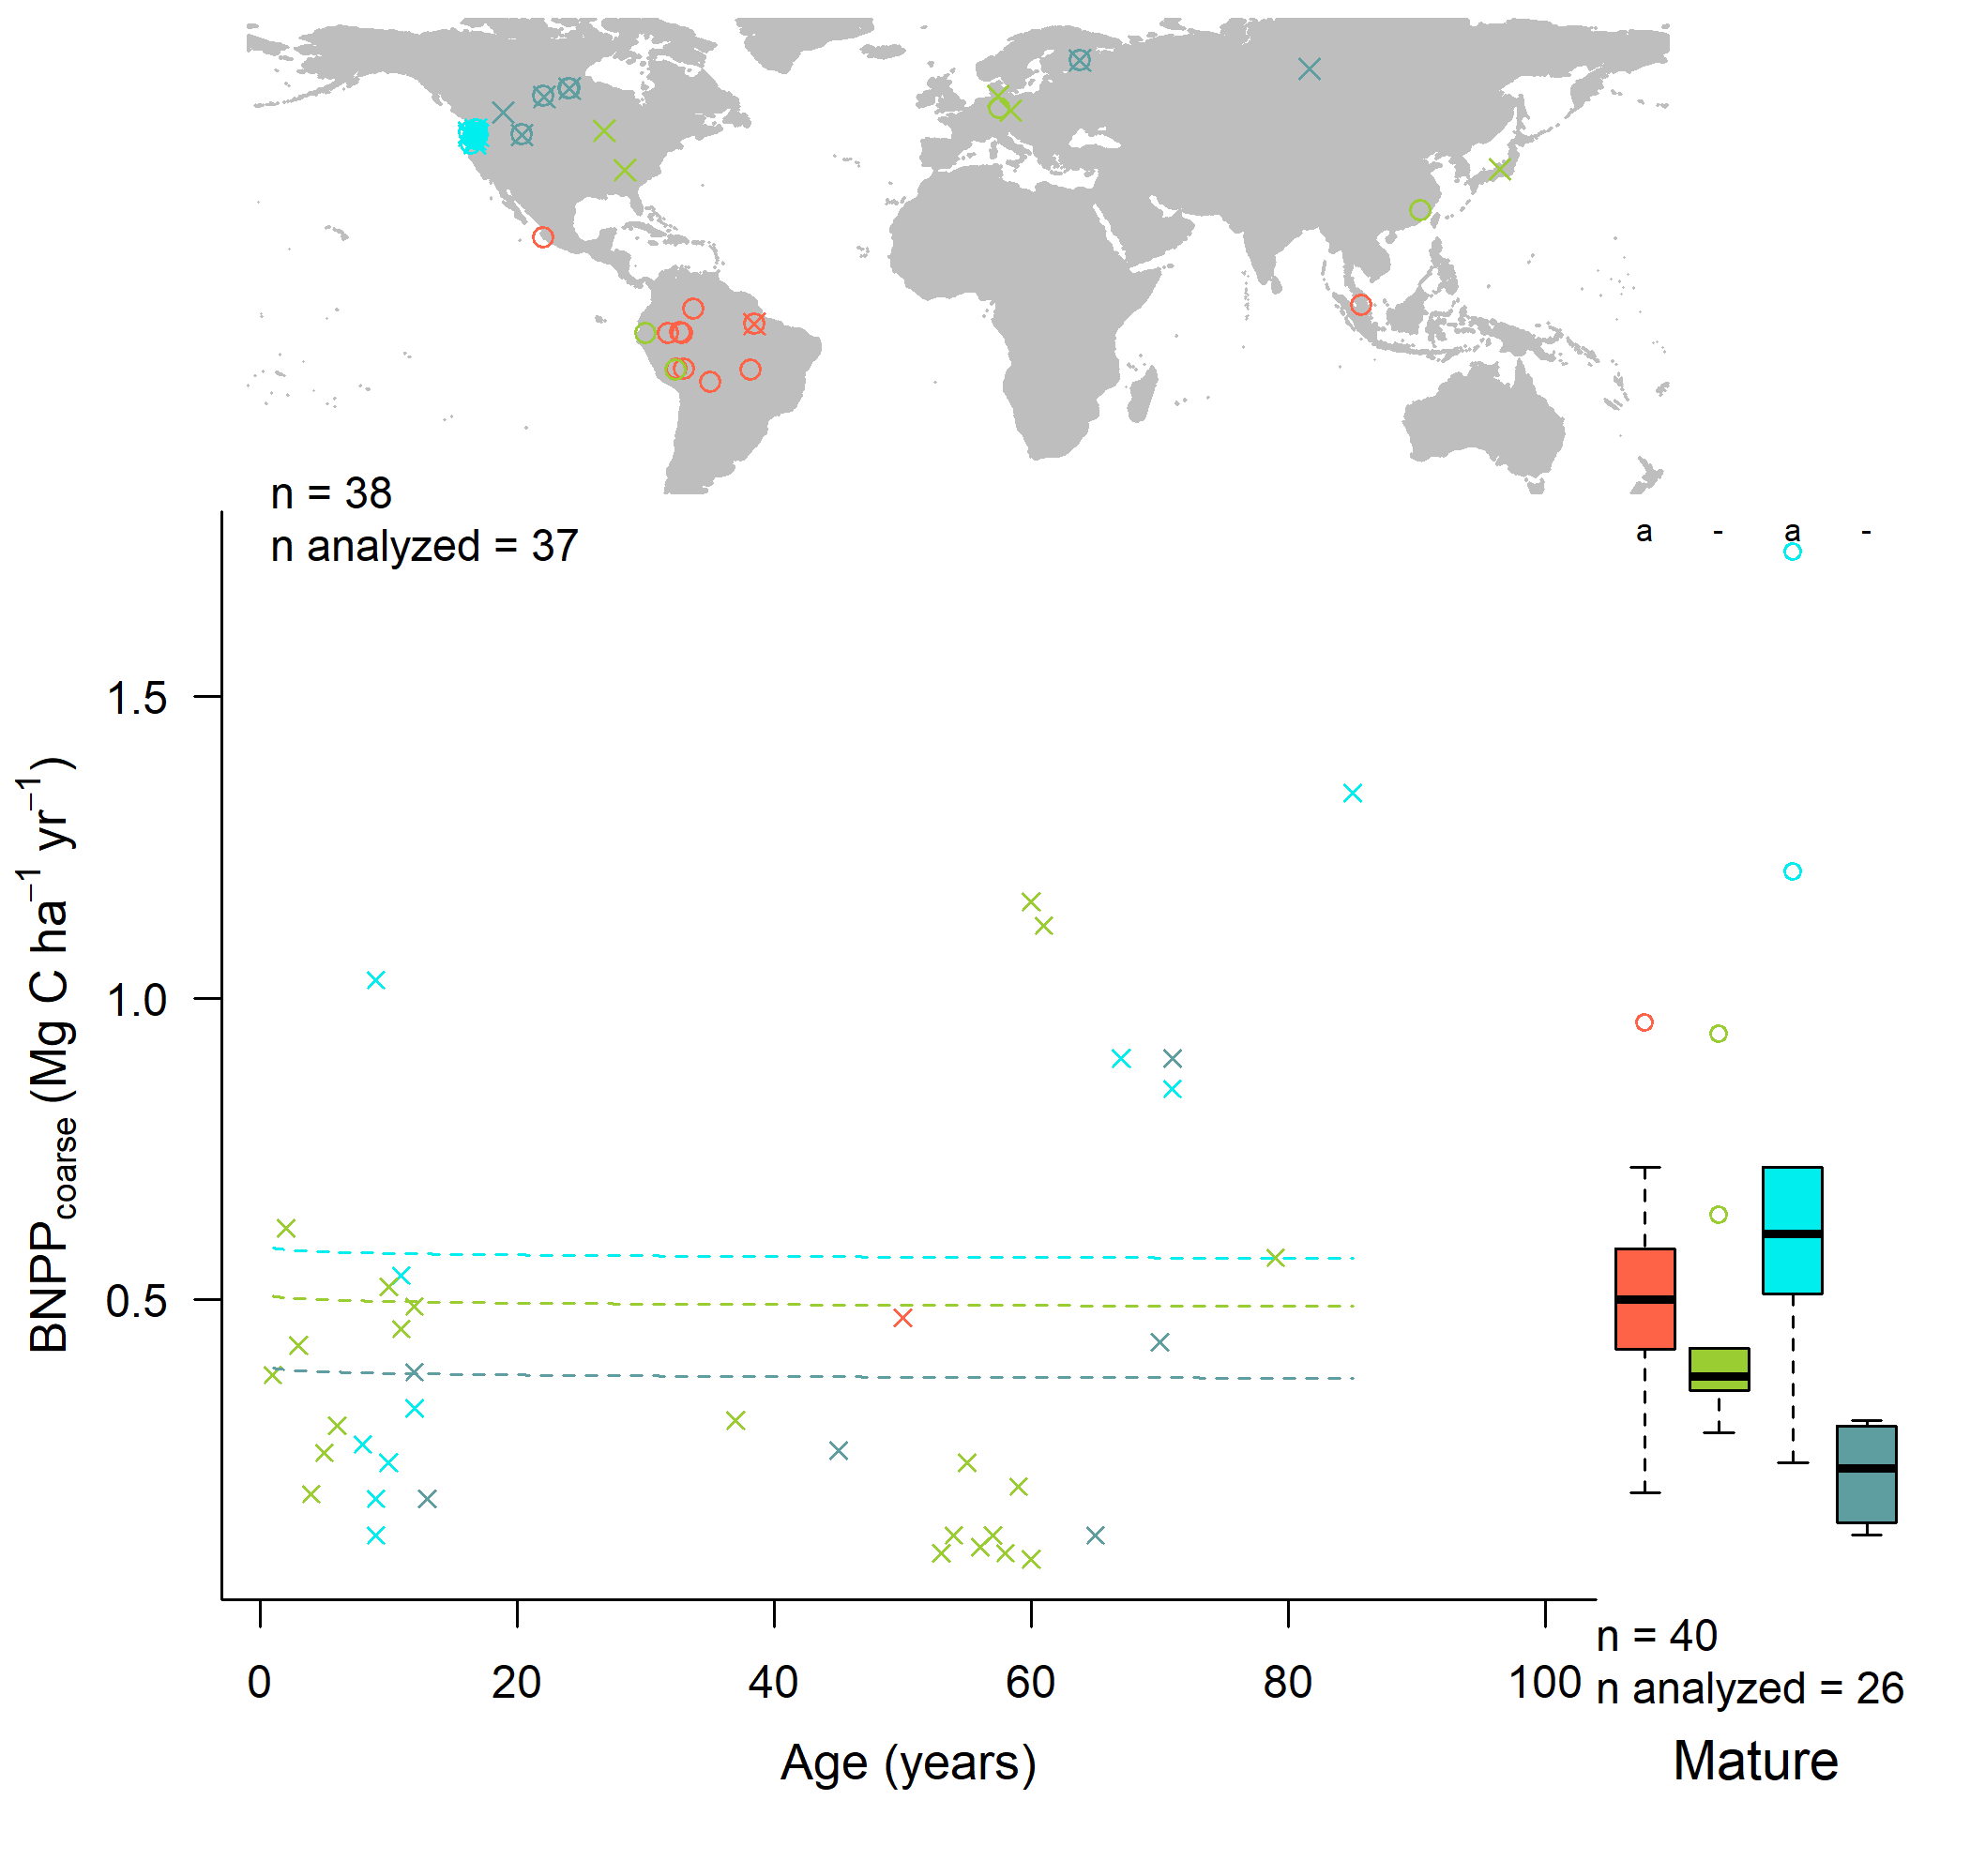
\includegraphics[width=1\linewidth]{tables_figures/age_trends/BNPP_coarse_with_map} 

}

\caption{Age trends and biome differences for $BNPP_{coarse}$. Map shows data sources ('$\times$' and '$\circ$' indicate young and mature stands, respectively). In each panel, the left scatterplot shows age trends in forests up to 100 years old, as characterized by a linear mixed effects model with fixed effects of log10(age) and biome. The fitted line indicates the effect of age (solid lines: significant at p<0.05, dashed lines: non-significant), and non-parallel lines indicate a significant log10(age) $\times$ biome interaction. Boxplot illustrates distribution across mature forests, with different letters indicating significant differences between biomes. Data from biomes that did not meet the sample size criteria (see Methods) are plotted, but lack regression lines (young forests) or test of differences across biomes (mature forests).}\label{fig:unnamed-chunk-17}
\end{figure}

\newpage

\hypertarget{figure-s15.-age-trends-and-biome-differences-for-bnpp_fine}{%
\subsection{\texorpdfstring{Figure S15. Age trends and biome differences
for
\(BNPP_{fine}\)}{Figure S15. Age trends and biome differences for BNPP\_\{fine\}}}\label{figure-s15.-age-trends-and-biome-differences-for-bnpp_fine}}

\begin{figure}[H]

{\centering 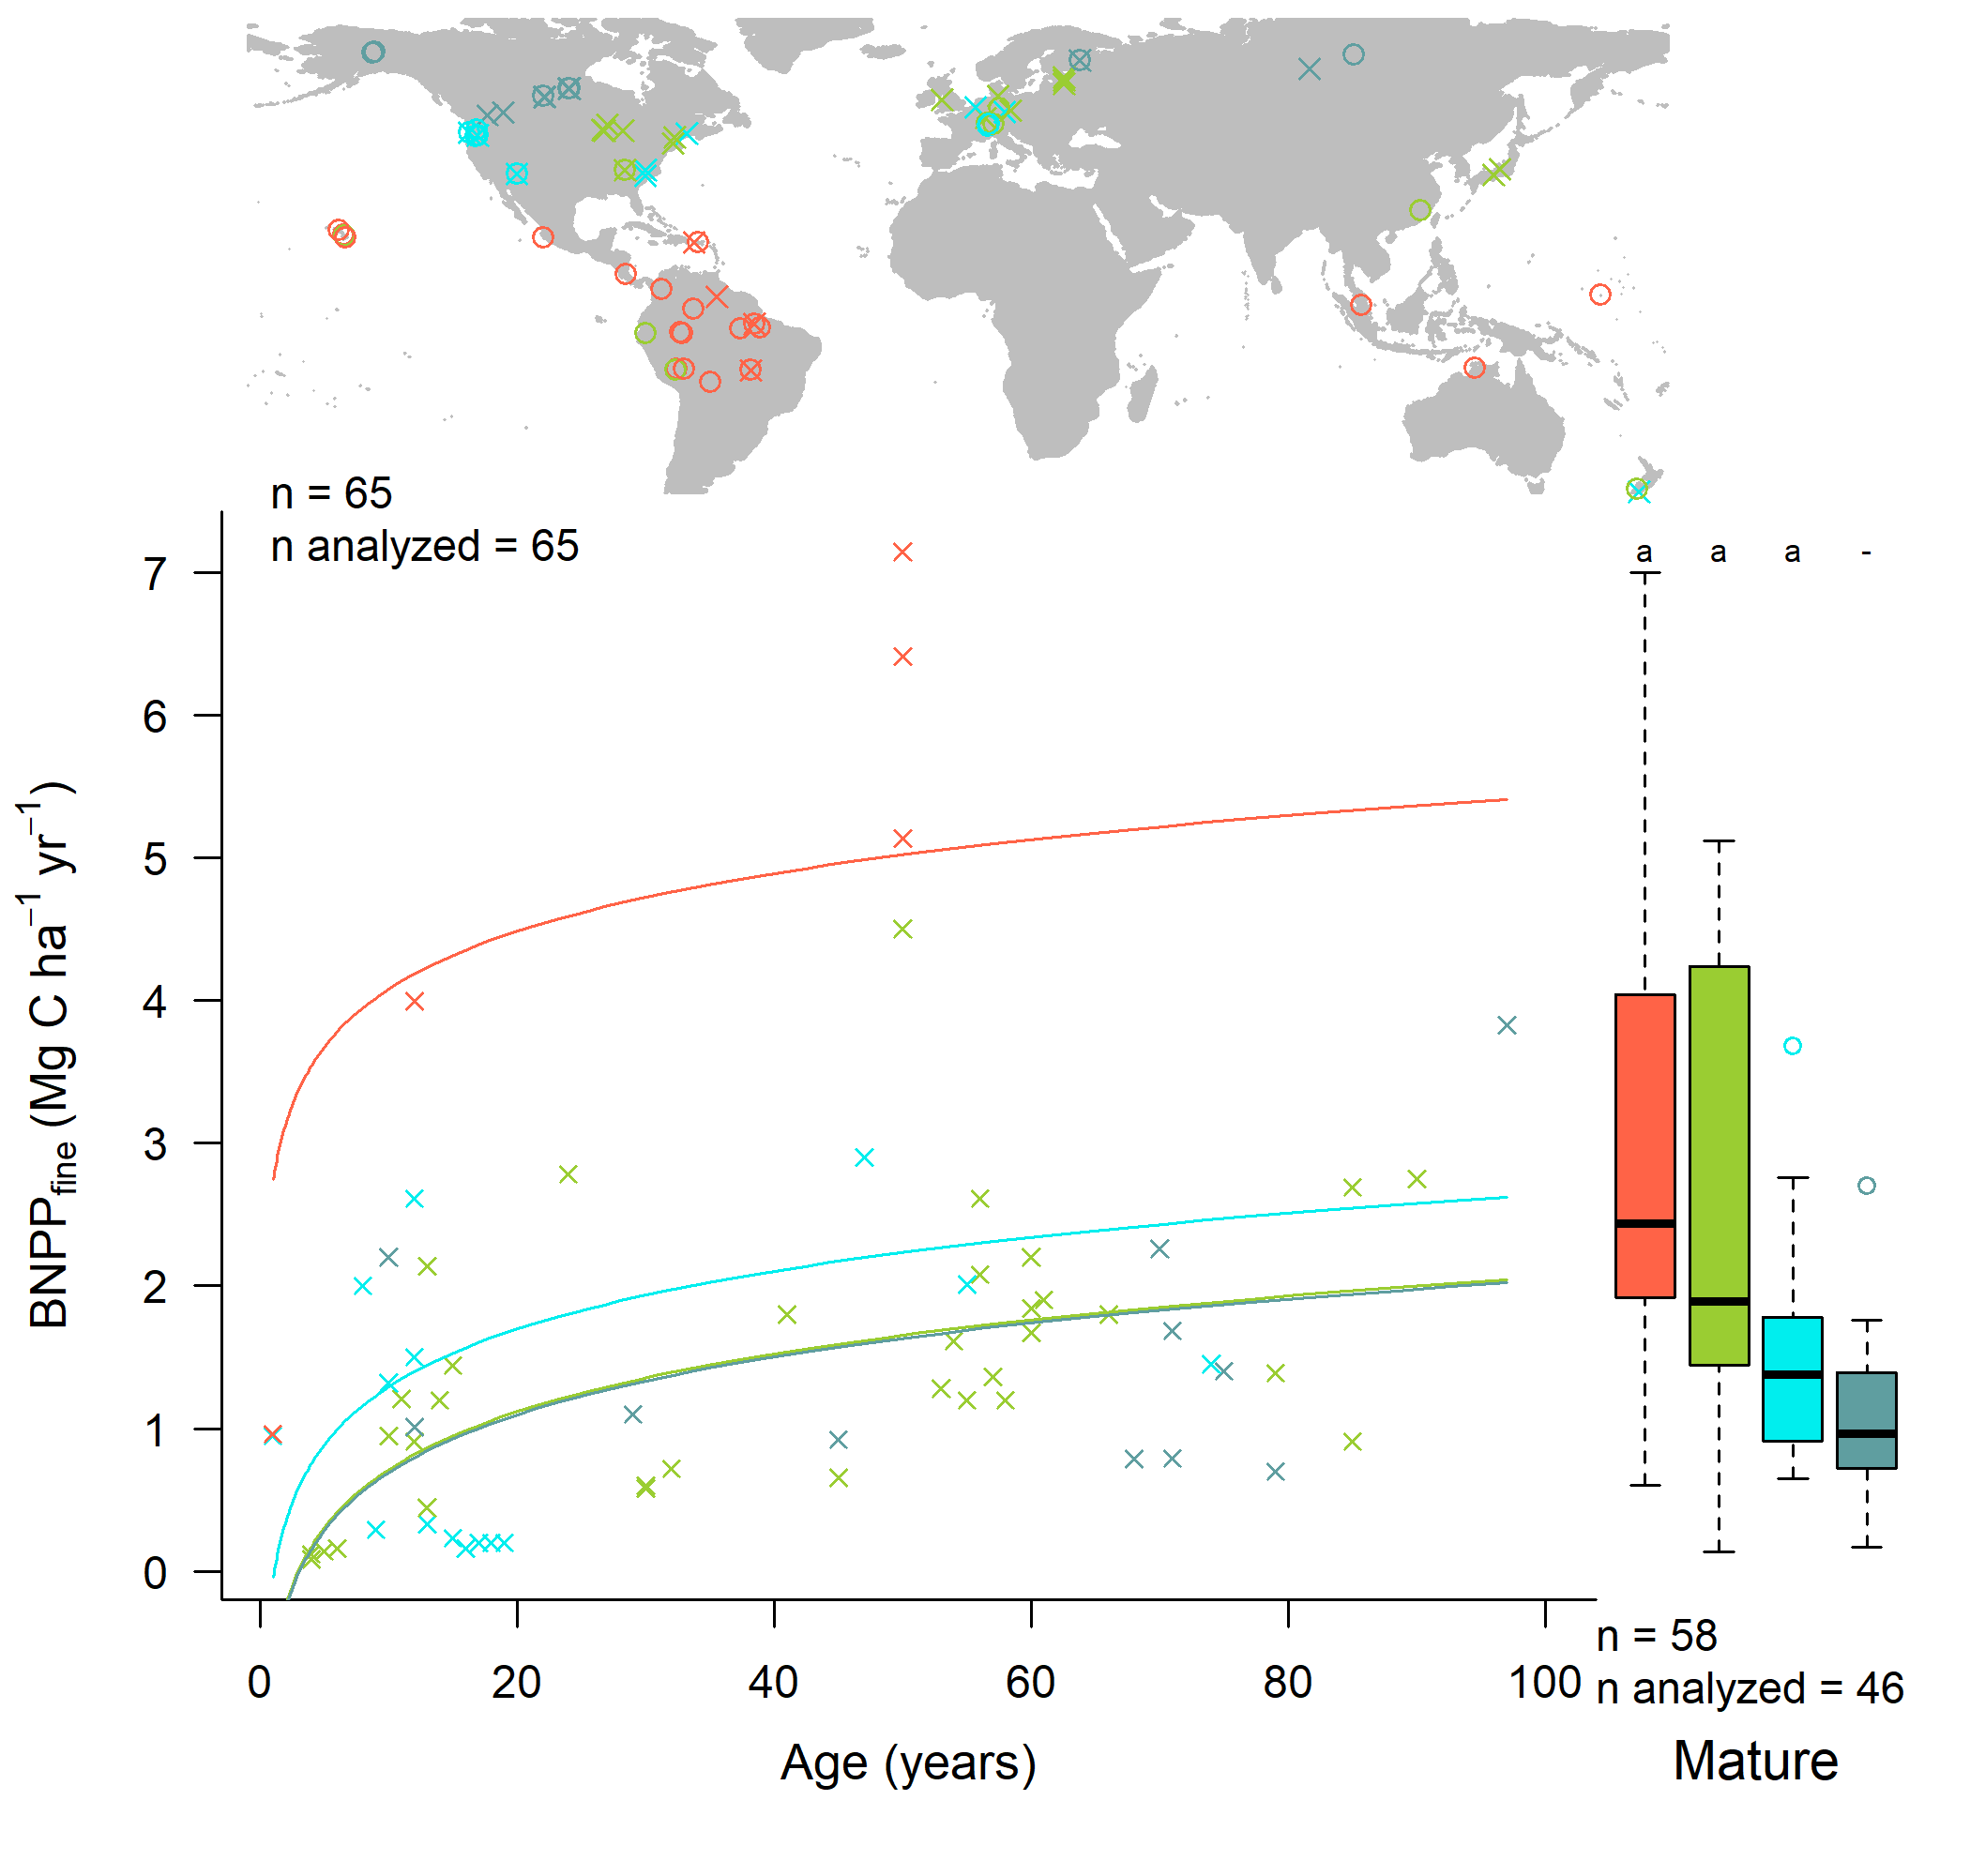
\includegraphics[width=1\linewidth]{tables_figures/age_trends/BNPP_fine_with_map} 

}

\caption{Age trends and biome differences for $BNPP_{fine}$. Map shows data sources ('$\times$' and '$\circ$' indicate young and mature stands, respectively). In each panel, the left scatterplot shows age trends in forests up to 100 years old, as characterized by a linear mixed effects model with fixed effects of log10(age) and biome. The fitted line indicates the effect of age (solid lines: significant at p<0.05, dashed lines: non-significant), and non-parallel lines indicate a significant log10(age) $\times$ biome interaction. Boxplot illustrates distribution across mature forests, with different letters indicating significant differences between biomes. Data from biomes that did not meet the sample size criteria (see Methods) are plotted, but lack regression lines (young forests) or test of differences across biomes (mature forests).}\label{fig:unnamed-chunk-18}
\end{figure}

\newpage

\hypertarget{figure-s16.-age-trends-and-biome-differences-for-r_eco}{%
\subsection{\texorpdfstring{Figure S16. Age trends and biome differences
for
\(R_{eco}\)}{Figure S16. Age trends and biome differences for R\_\{eco\}}}\label{figure-s16.-age-trends-and-biome-differences-for-r_eco}}

\begin{figure}[H]

{\centering 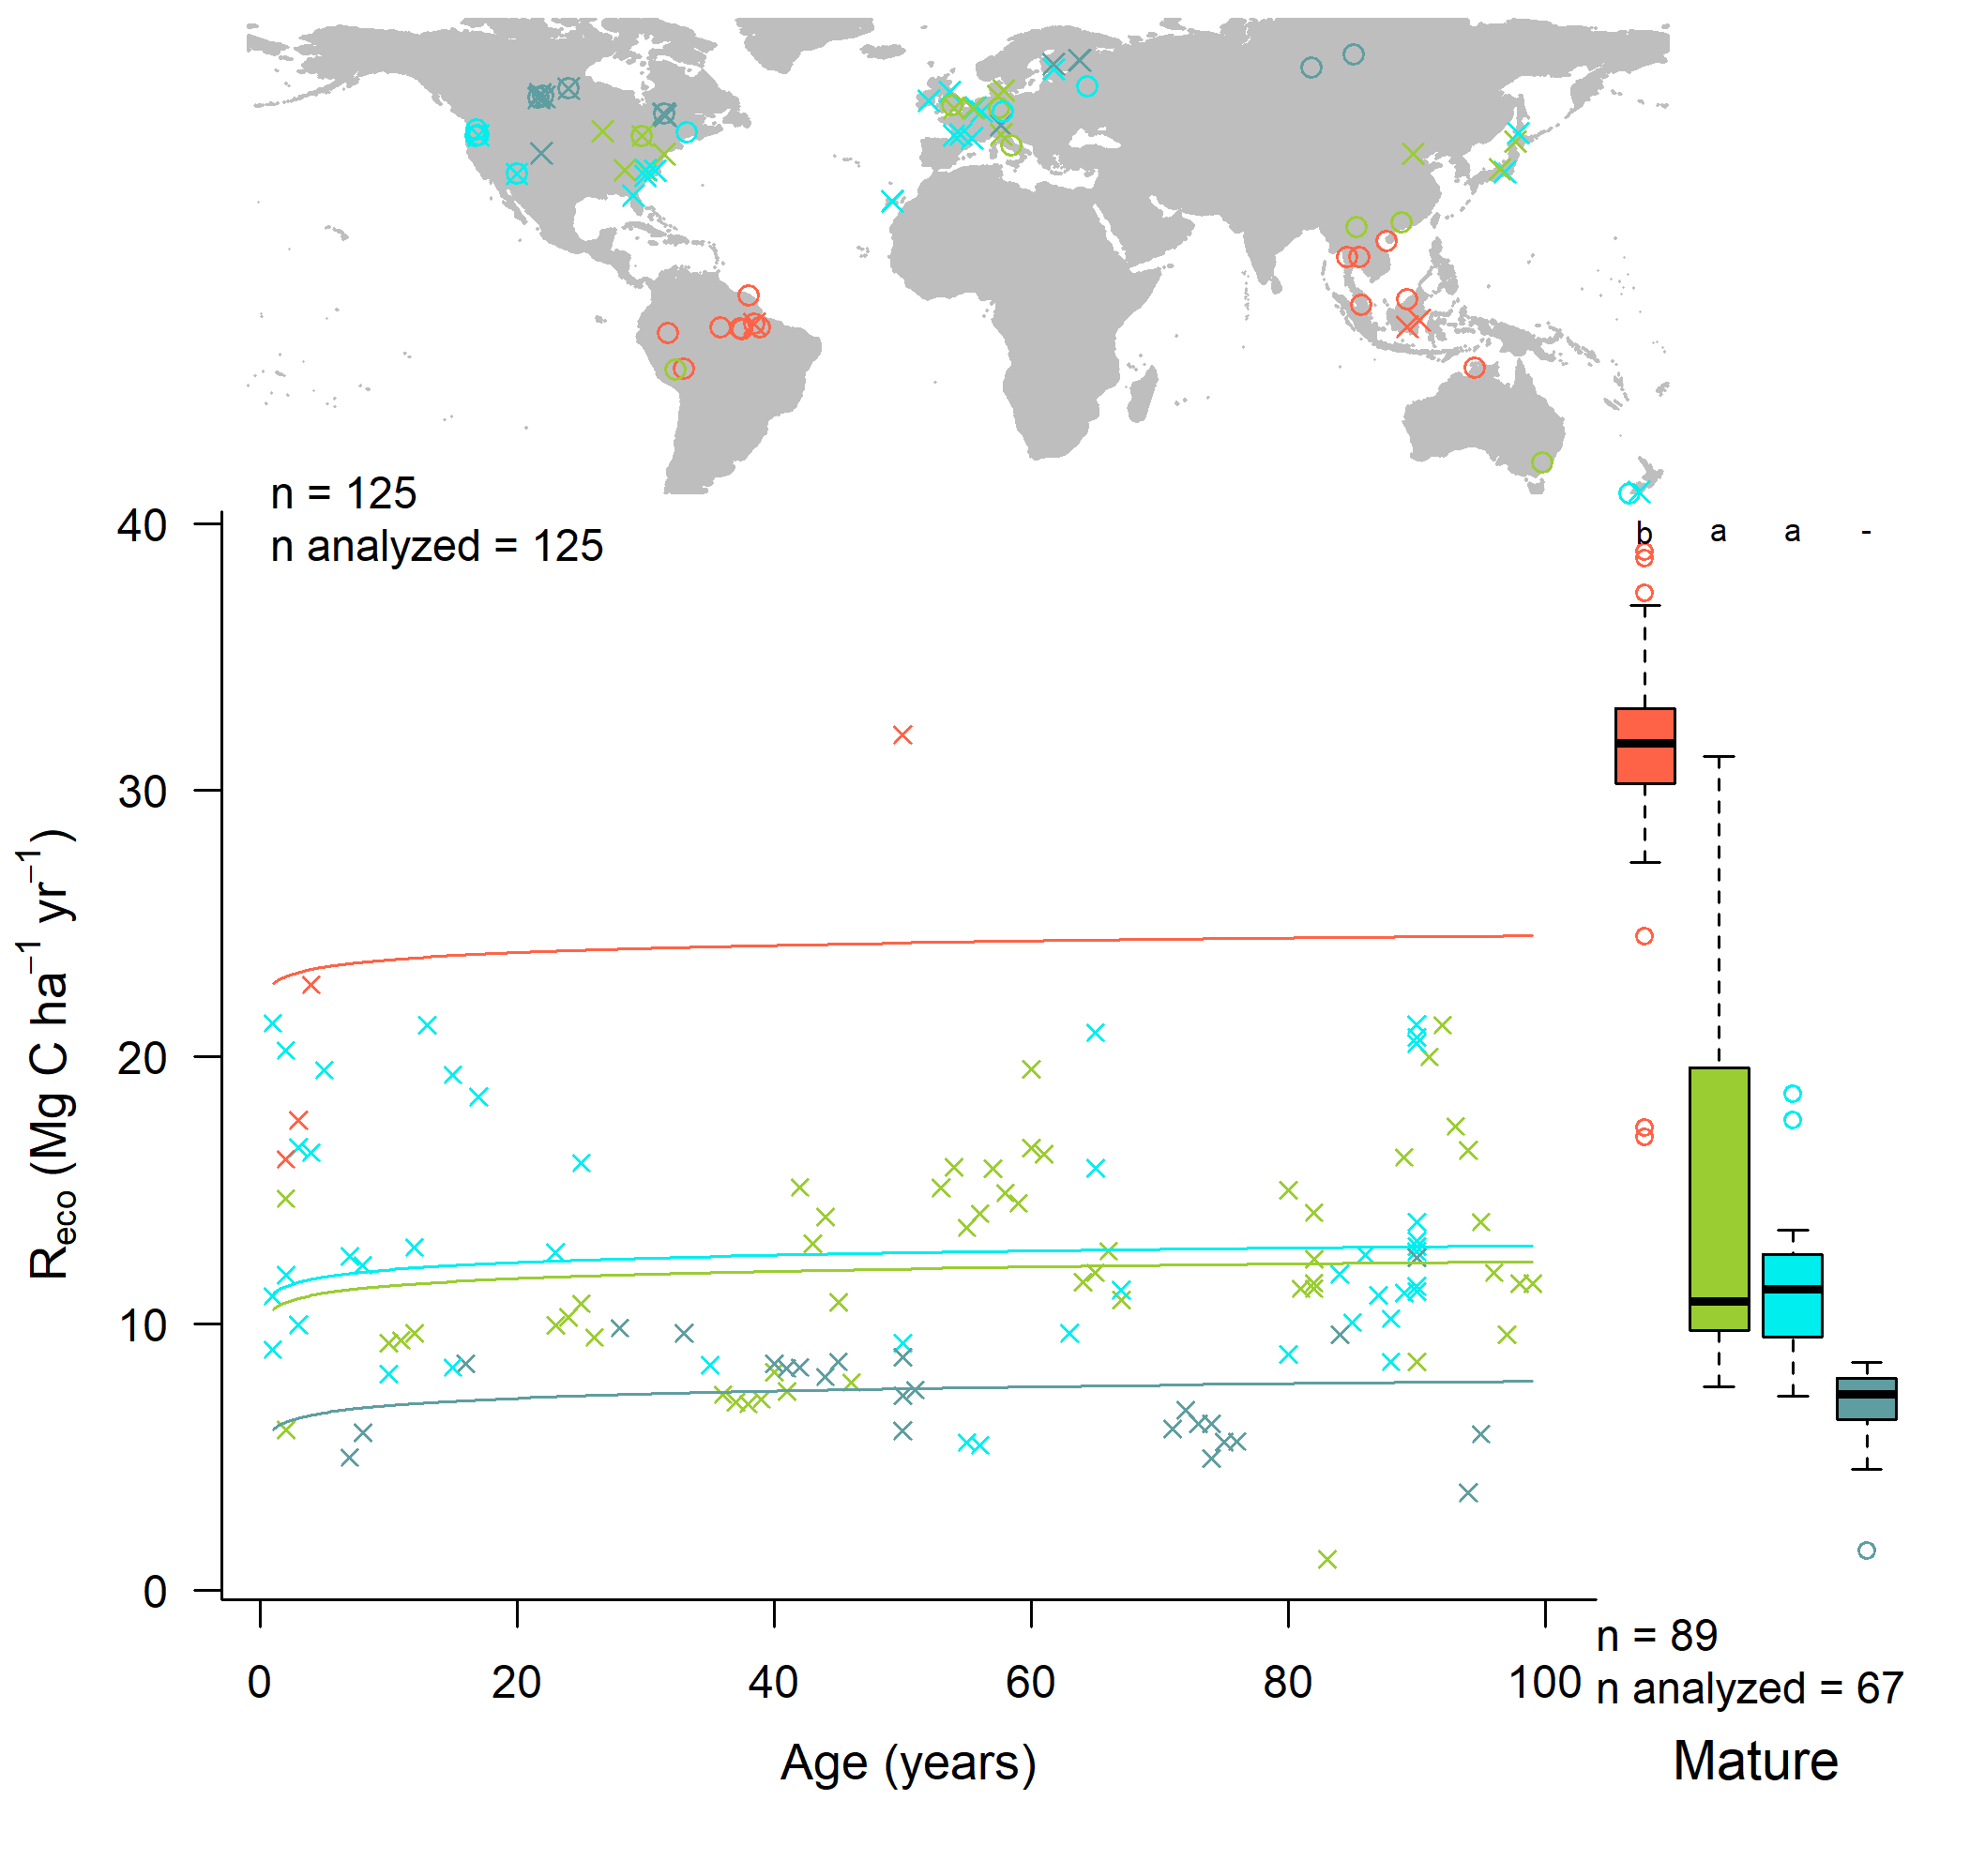
\includegraphics[width=1\linewidth]{tables_figures/age_trends/R_eco_with_map} 

}

\caption{Age trends and biome differences for $R_{eco}$. Map shows data sources ('$\times$' and '$\circ$' indicate young and mature stands, respectively). In each panel, the left scatterplot shows age trends in forests up to 100 years old, as characterized by a linear mixed effects model with fixed effects of log10(age) and biome. The fitted line indicates the effect of age (solid lines: significant at p<0.05, dashed lines: non-significant), and non-parallel lines indicate a significant log10(age) $\times$ biome interaction. Boxplot illustrates distribution across mature forests, with different letters indicating significant differences between biomes. Data from biomes that did not meet the sample size criteria (see Methods) are plotted, but lack regression lines (young forests) or test of differences across biomes (mature forests).}\label{fig:unnamed-chunk-19}
\end{figure}

\newpage

\hypertarget{figure-s17.-age-trends-and-biome-differences-for-r_root}{%
\subsection{\texorpdfstring{Figure S17. Age trends and biome differences
for
\(R_{root}\)}{Figure S17. Age trends and biome differences for R\_\{root\}}}\label{figure-s17.-age-trends-and-biome-differences-for-r_root}}

\begin{figure}[H]

{\centering 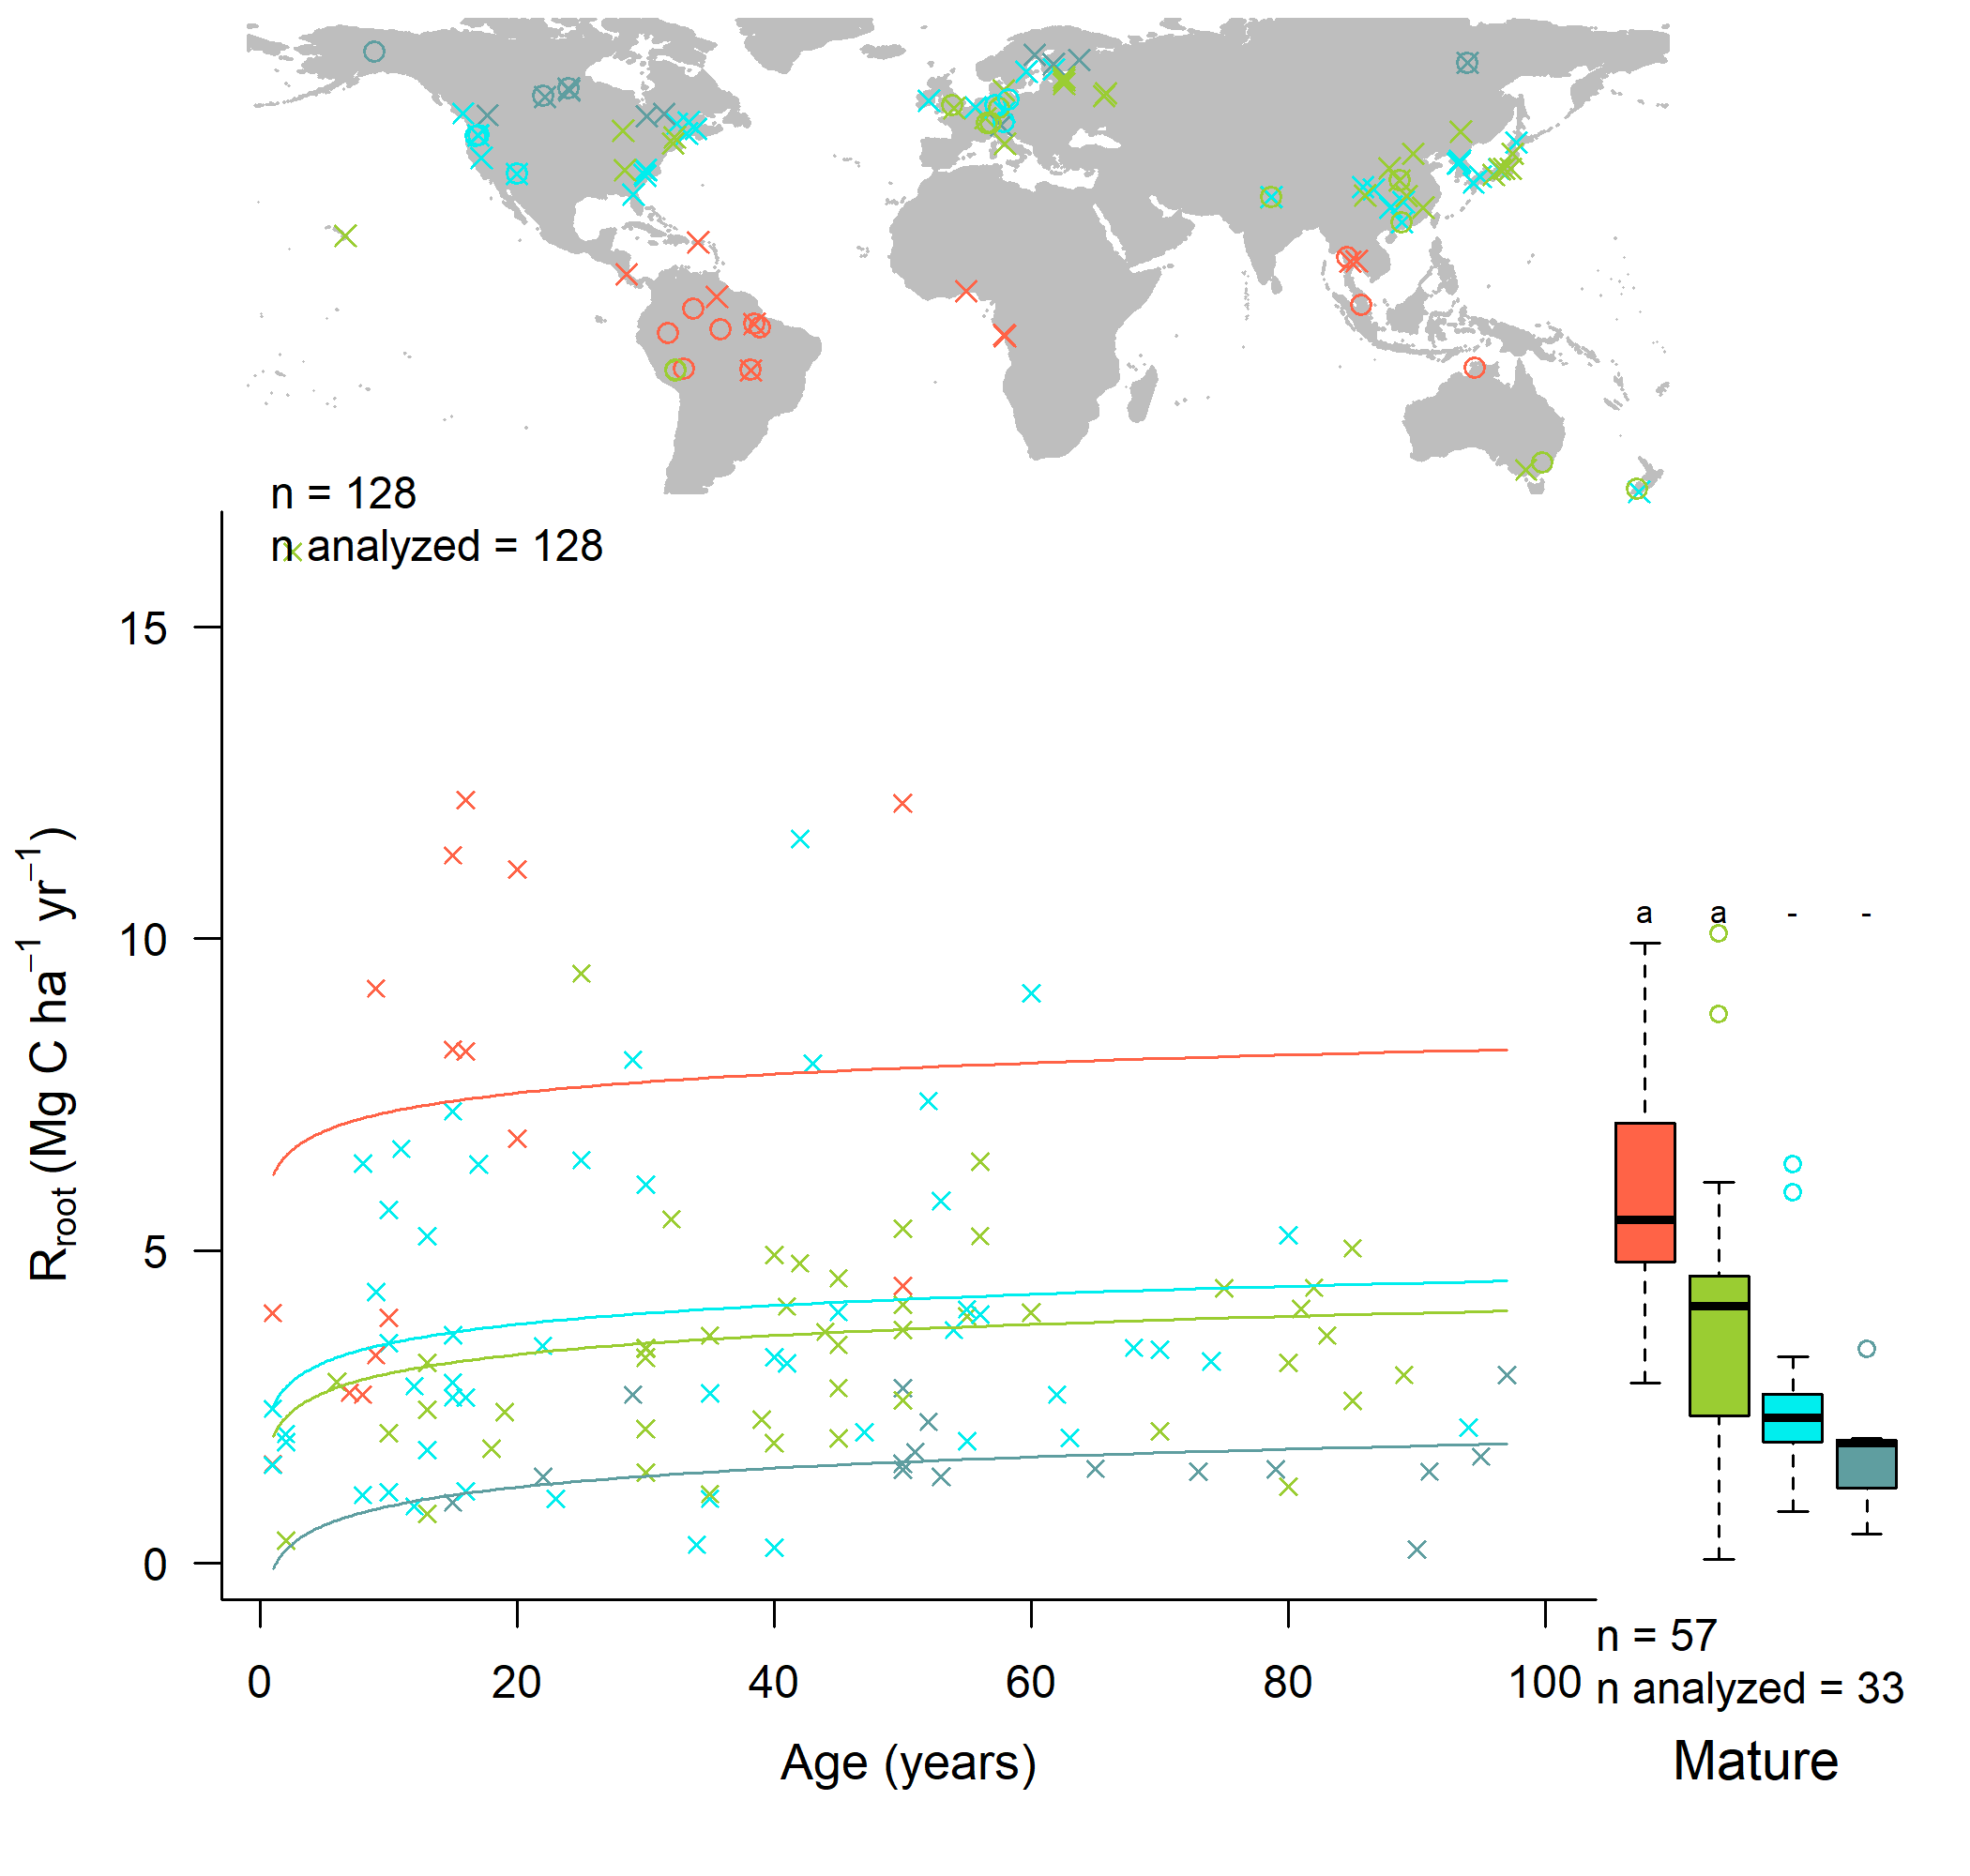
\includegraphics[width=1\linewidth]{tables_figures/age_trends/R_root_with_map} 

}

\caption{Age trends and biome differences for $R_{root}$. Map shows data sources ('$\times$' and '$\circ$' indicate young and mature stands, respectively). In each panel, the left scatterplot shows age trends in forests up to 100 years old, as characterized by a linear mixed effects model with fixed effects of log10(age) and biome. The fitted line indicates the effect of age (solid lines: significant at p<0.05, dashed lines: non-significant), and non-parallel lines indicate a significant log10(age) $\times$ biome interaction. Boxplot illustrates distribution across mature forests, with different letters indicating significant differences between biomes. Data from biomes that did not meet the sample size criteria (see Methods) are plotted, but lack regression lines (young forests) or test of differences across biomes (mature forests).}\label{fig:unnamed-chunk-20}
\end{figure}

\newpage

\hypertarget{figure-s18.-age-trends-and-biome-differences-for-r_soil}{%
\subsection{\texorpdfstring{Figure S18. Age trends and biome differences
for
\(R_{soil}\)}{Figure S18. Age trends and biome differences for R\_\{soil\}}}\label{figure-s18.-age-trends-and-biome-differences-for-r_soil}}

\begin{figure}[H]

{\centering 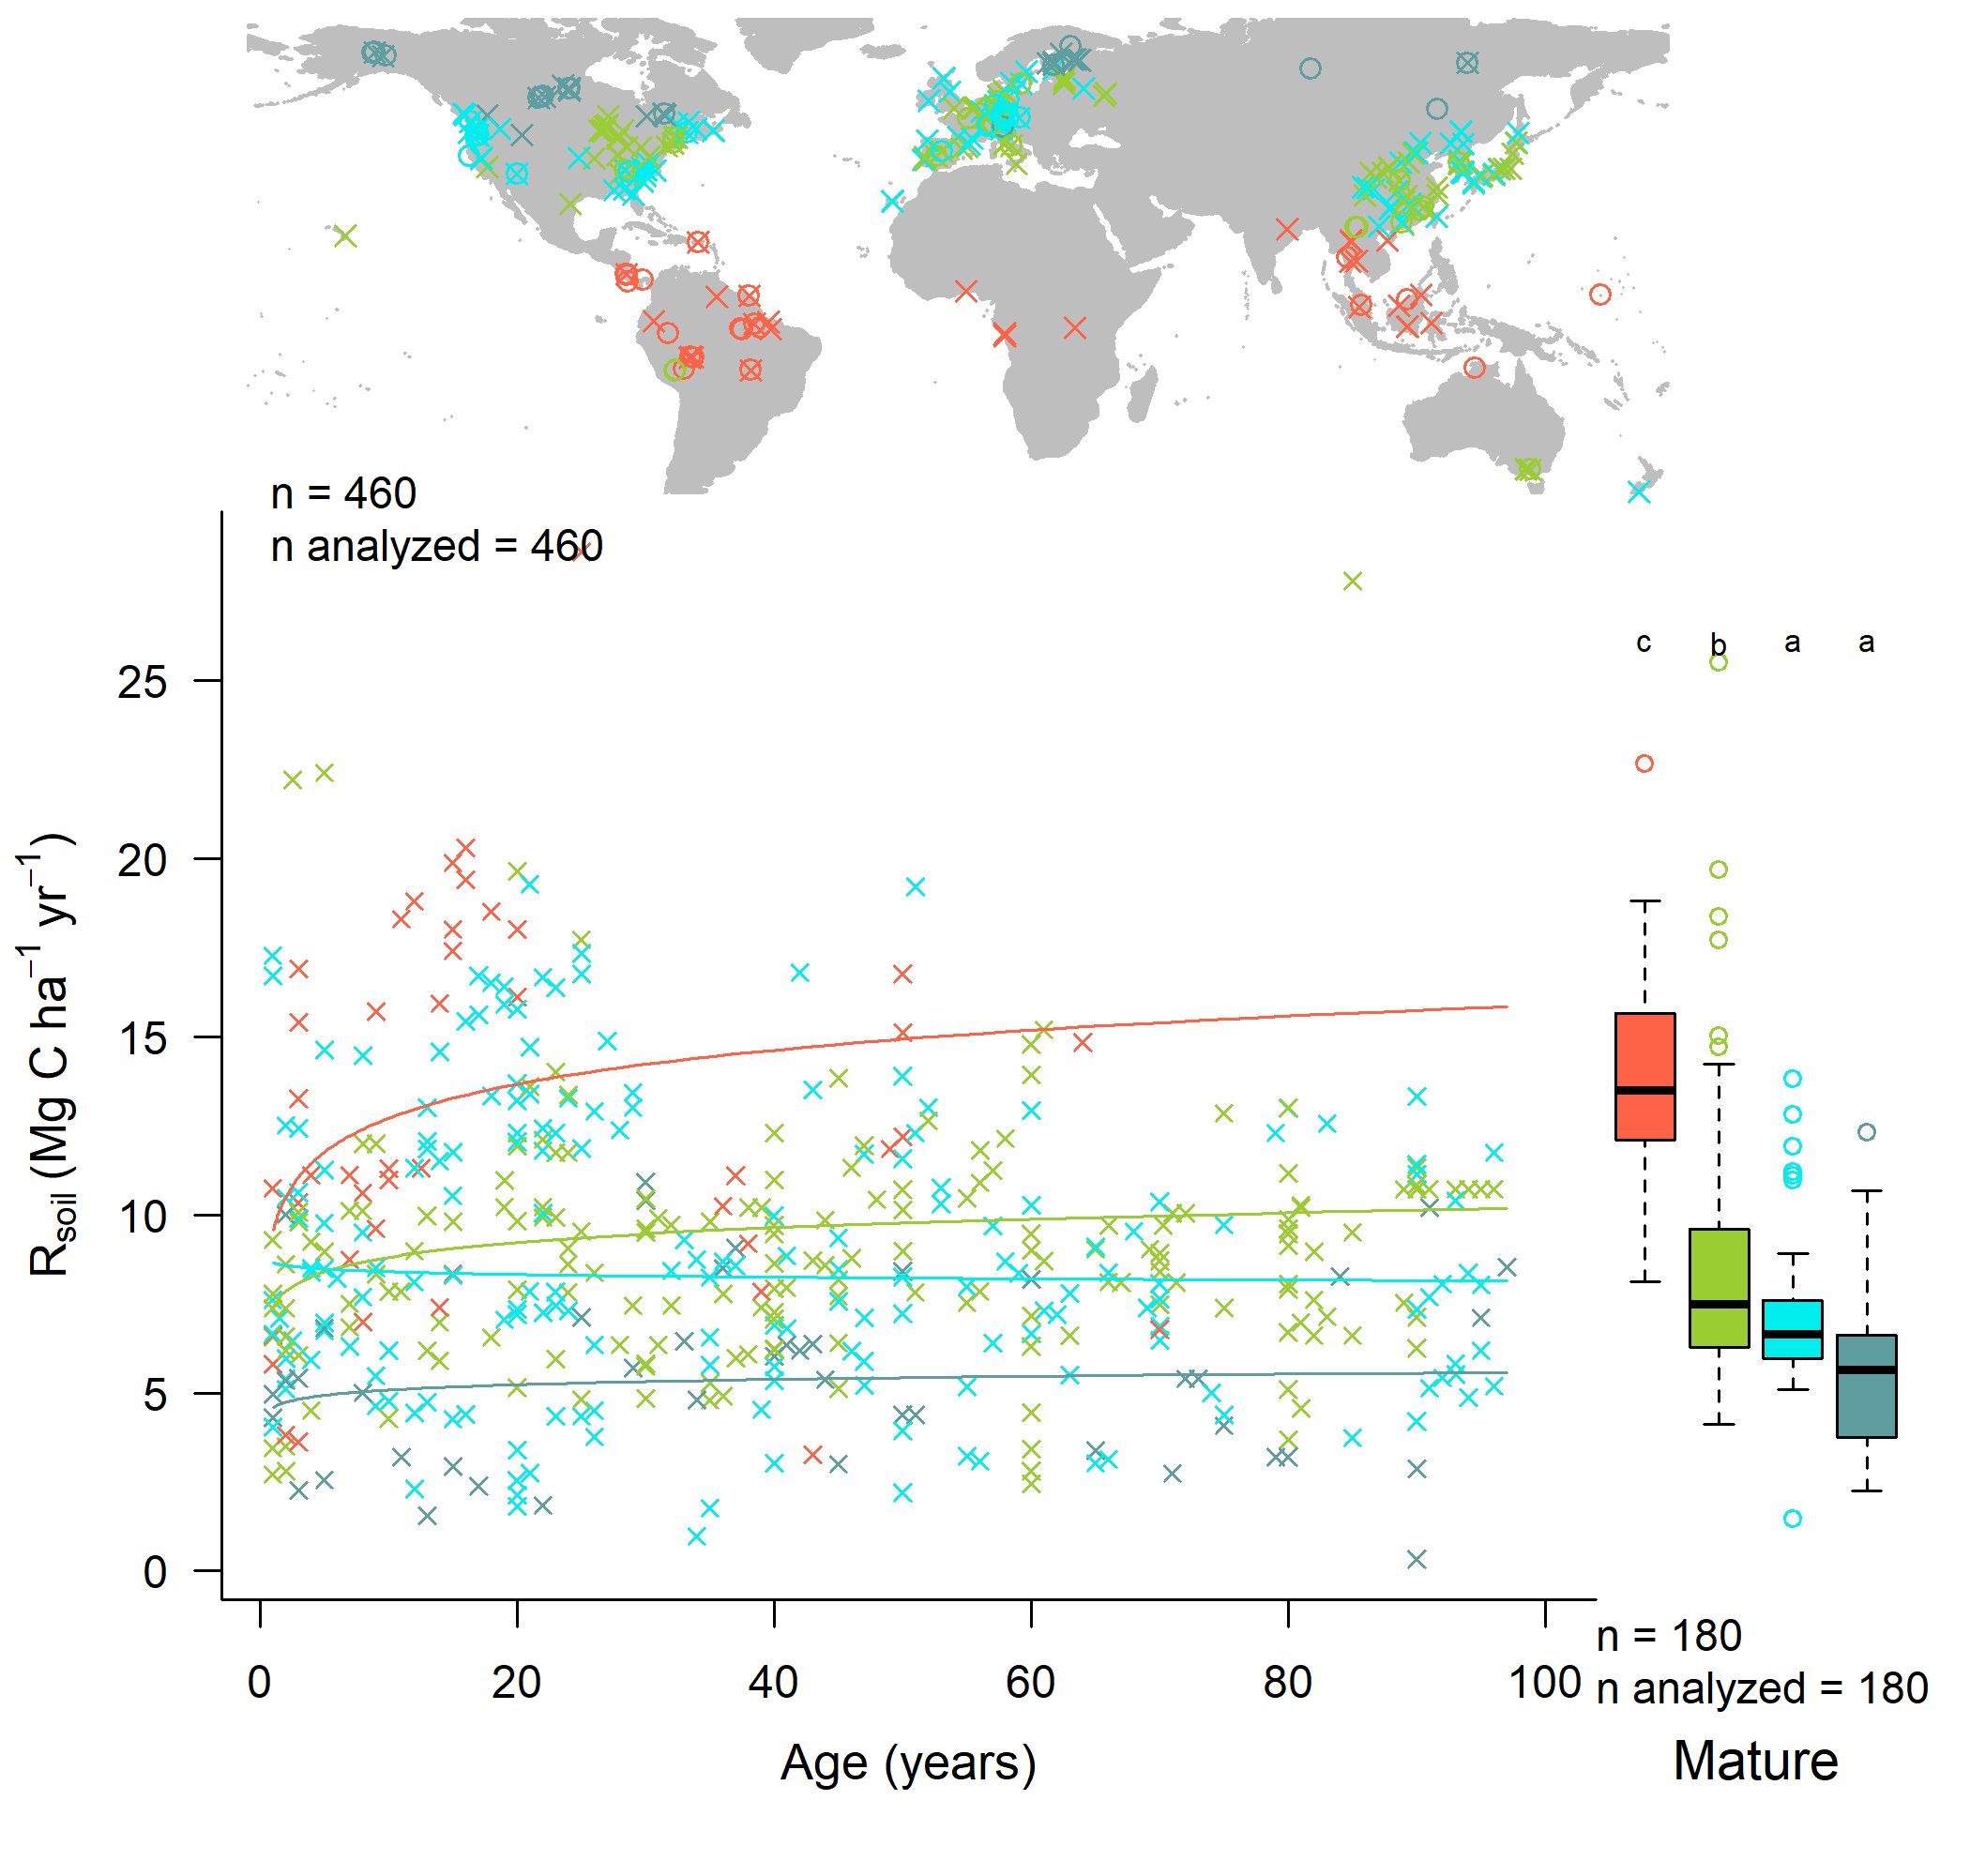
\includegraphics[width=1\linewidth]{tables_figures/age_trends/R_soil_with_map} 

}

\caption{Age trends and biome differences for $R_{soil}$. Map shows data sources ('$\times$' and '$\circ$' indicate young and mature stands, respectively). In each panel, the left scatterplot shows age trends in forests up to 100 years old, as characterized by a linear mixed effects model with fixed effects of log10(age) and biome. The fitted line indicates the effect of age (solid lines: significant at p<0.05, dashed lines: non-significant), and non-parallel lines indicate a significant log10(age) $\times$ biome interaction. Boxplot illustrates distribution across mature forests, with different letters indicating significant differences between biomes. Data from biomes that did not meet the sample size criteria (see Methods) are plotted, but lack regression lines (young forests) or test of differences across biomes (mature forests).}\label{fig:unnamed-chunk-21}
\end{figure}

\newpage

\hypertarget{figure-s19.-age-trends-and-biome-differences-for-r_het-soil}{%
\subsection{\texorpdfstring{Figure S19. Age trends and biome differences
for
\(R_{het-soil}\)}{Figure S19. Age trends and biome differences for R\_\{het-soil\}}}\label{figure-s19.-age-trends-and-biome-differences-for-r_het-soil}}

\begin{figure}[H]

{\centering 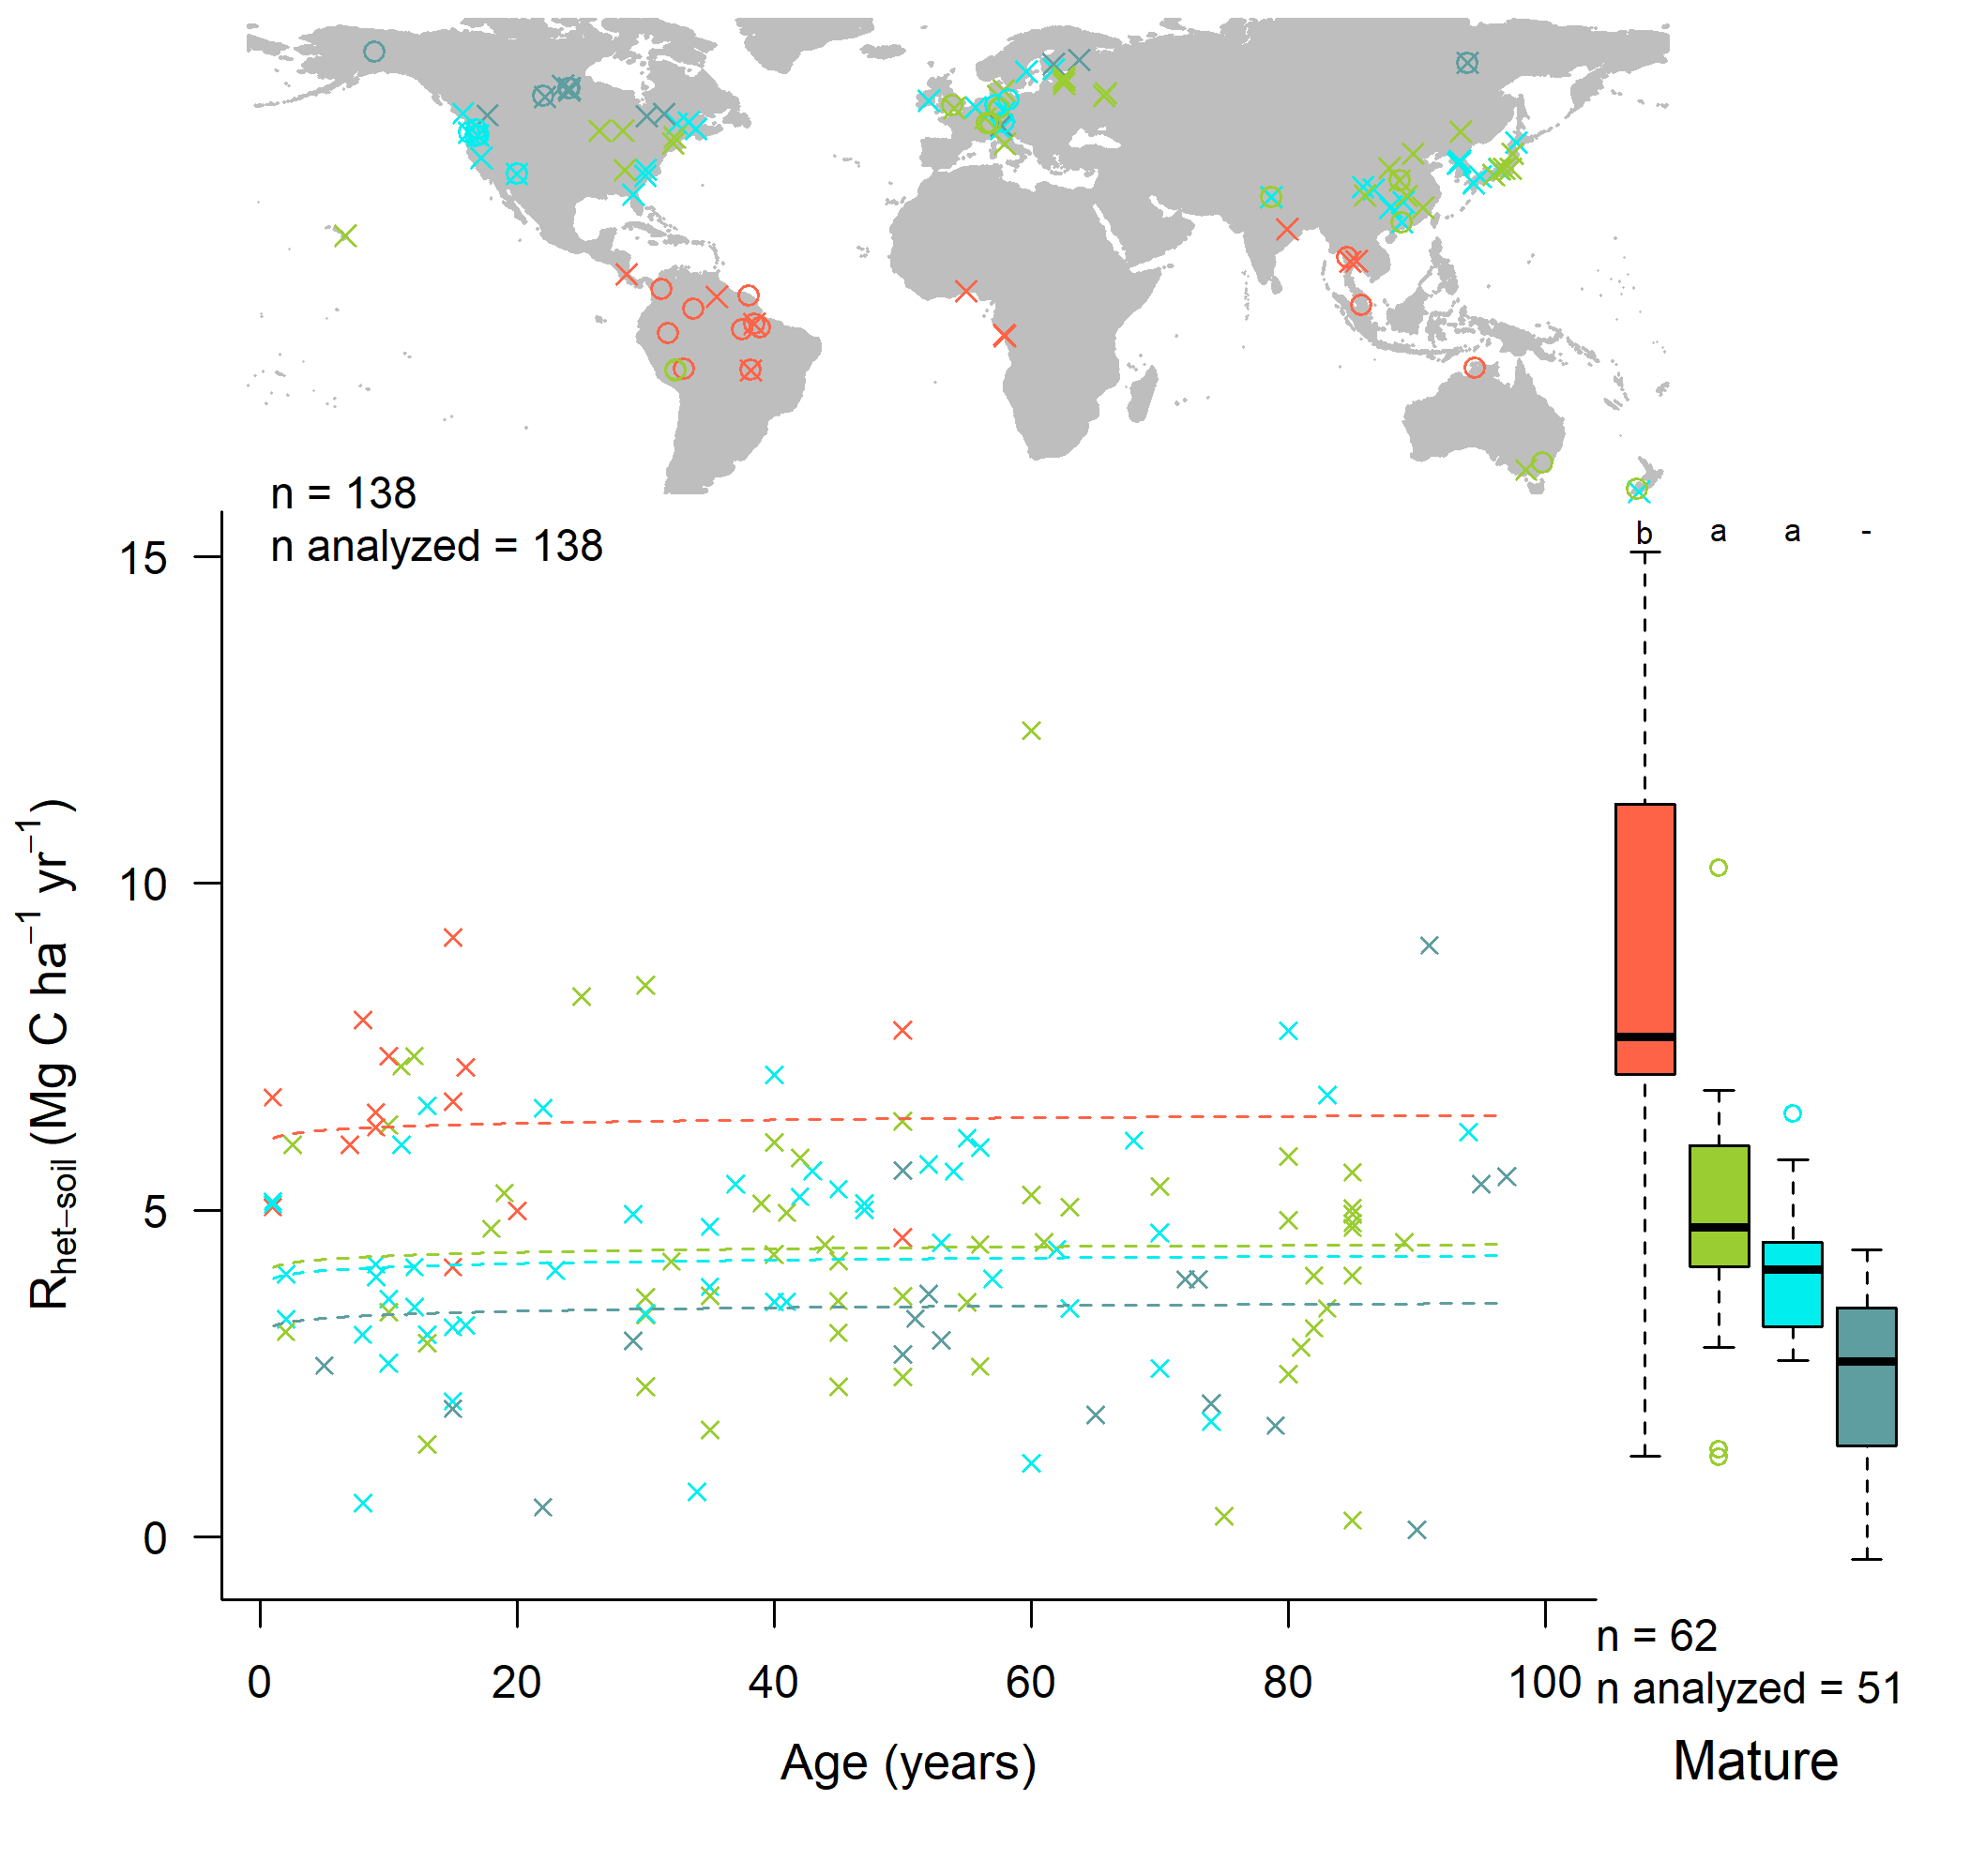
\includegraphics[width=1\linewidth]{tables_figures/age_trends/R_het_soil_with_map} 

}

\caption{Age trends and biome differences for $R_{het-soil}$. Map shows data sources ('$\times$' and '$\circ$' indicate young and mature stands, respectively). In each panel, the left scatterplot shows age trends in forests up to 100 years old, as characterized by a linear mixed effects model with fixed effects of log10(age) and biome. The fitted line indicates the effect of age (solid lines: significant at p<0.05, dashed lines: non-significant), and non-parallel lines indicate a significant log10(age) $\times$ biome interaction. Boxplot illustrates distribution across mature forests, with different letters indicating significant differences between biomes. Data from biomes that did not meet the sample size criteria (see Methods) are plotted, but lack regression lines (young forests) or test of differences across biomes (mature forests).}\label{fig:unnamed-chunk-22}
\end{figure}

\newpage

\hypertarget{figure-s20.-age-trends-and-biome-differences-for-b_tot}{%
\subsection{\texorpdfstring{Figure S20. Age trends and biome differences
for
\(B_{tot}\)}{Figure S20. Age trends and biome differences for B\_\{tot\}}}\label{figure-s20.-age-trends-and-biome-differences-for-b_tot}}

\begin{figure}[H]

{\centering 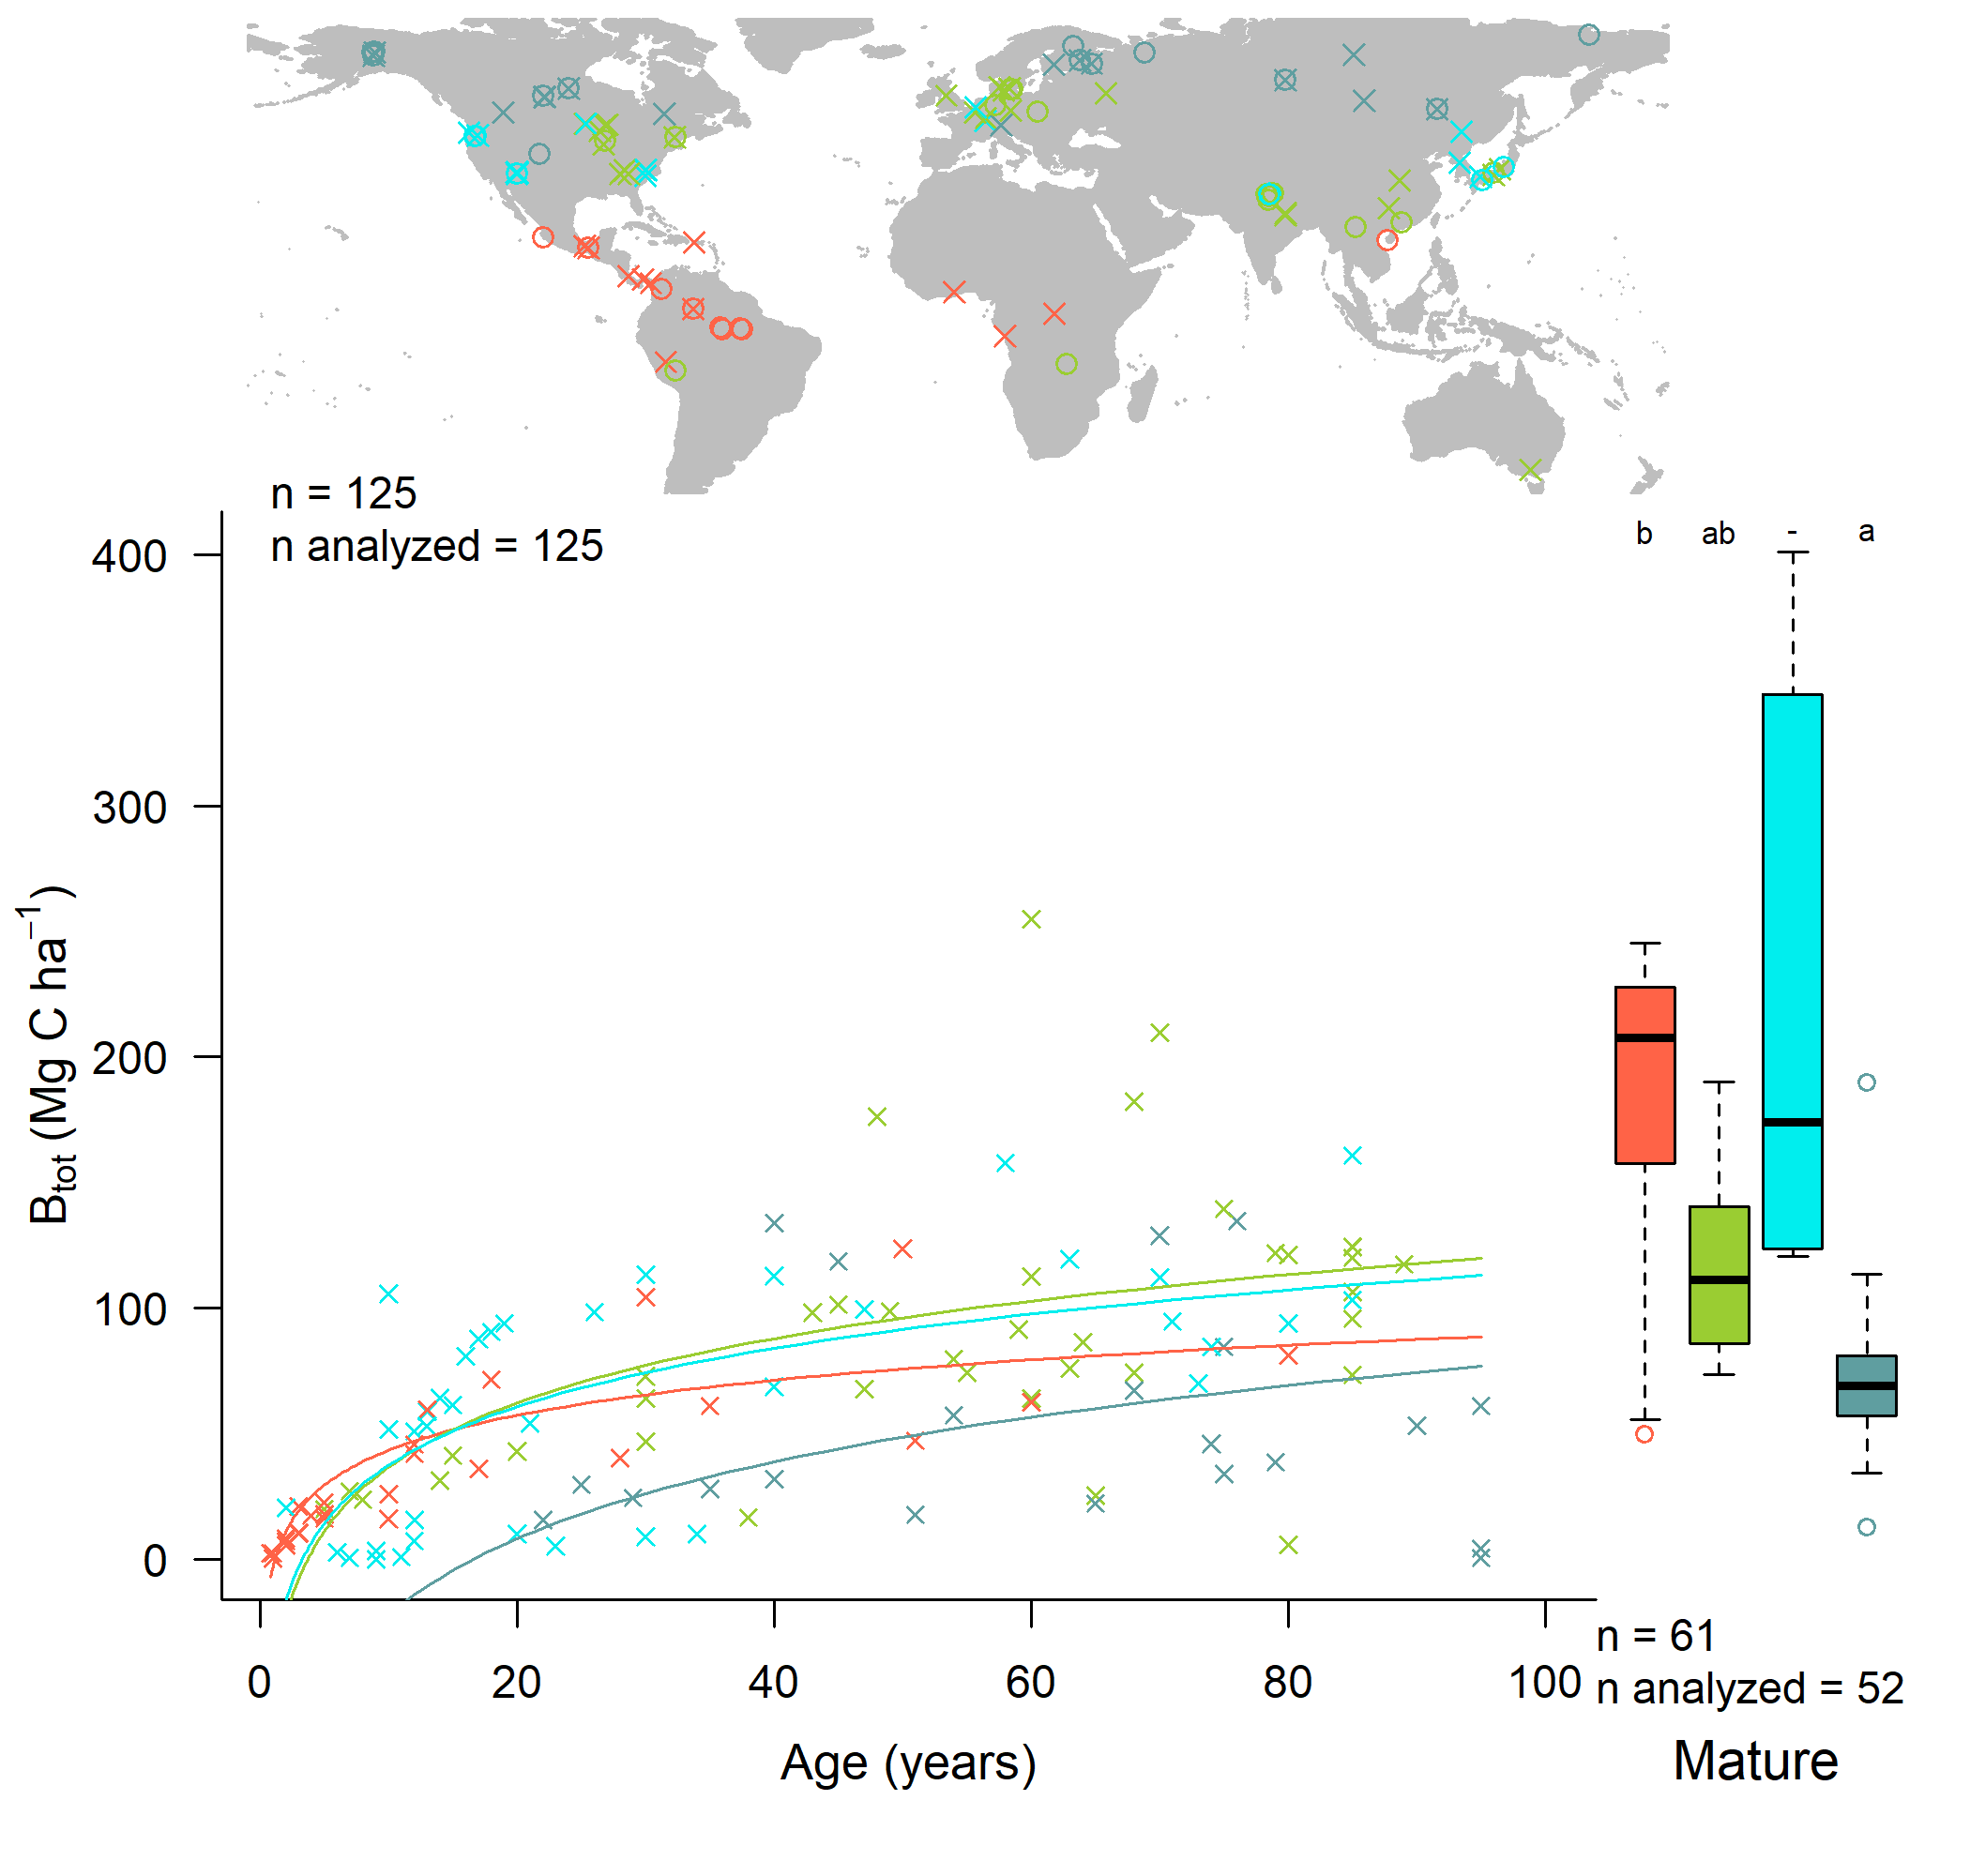
\includegraphics[width=1\linewidth]{tables_figures/age_trends/biomass_with_map} 

}

\caption{Age trends and biome differences for $B_{tot}$. Map shows data sources ('$\times$' and '$\circ$' indicate young and mature stands, respectively). In each panel, the left scatterplot shows age trends in forests up to 100 years old, as characterized by a linear mixed effects model with fixed effects of log10(age) and biome. The fitted line indicates the effect of age (solid lines: significant at p<0.05, dashed lines: non-significant), and non-parallel lines indicate a significant log10(age) $\times$ biome interaction. Boxplot illustrates distribution across mature forests, with different letters indicating significant differences between biomes. Data from biomes that did not meet the sample size criteria (see Methods) are plotted, but lack regression lines (young forests) or test of differences across biomes (mature forests).}\label{fig:unnamed-chunk-23}
\end{figure}

\newpage

\hypertarget{figure-s21.-age-trends-and-biome-differences-for-b_ag}{%
\subsection{\texorpdfstring{Figure S21. Age trends and biome differences
for
\(B_{ag}\)}{Figure S21. Age trends and biome differences for B\_\{ag\}}}\label{figure-s21.-age-trends-and-biome-differences-for-b_ag}}

\begin{figure}[H]

{\centering 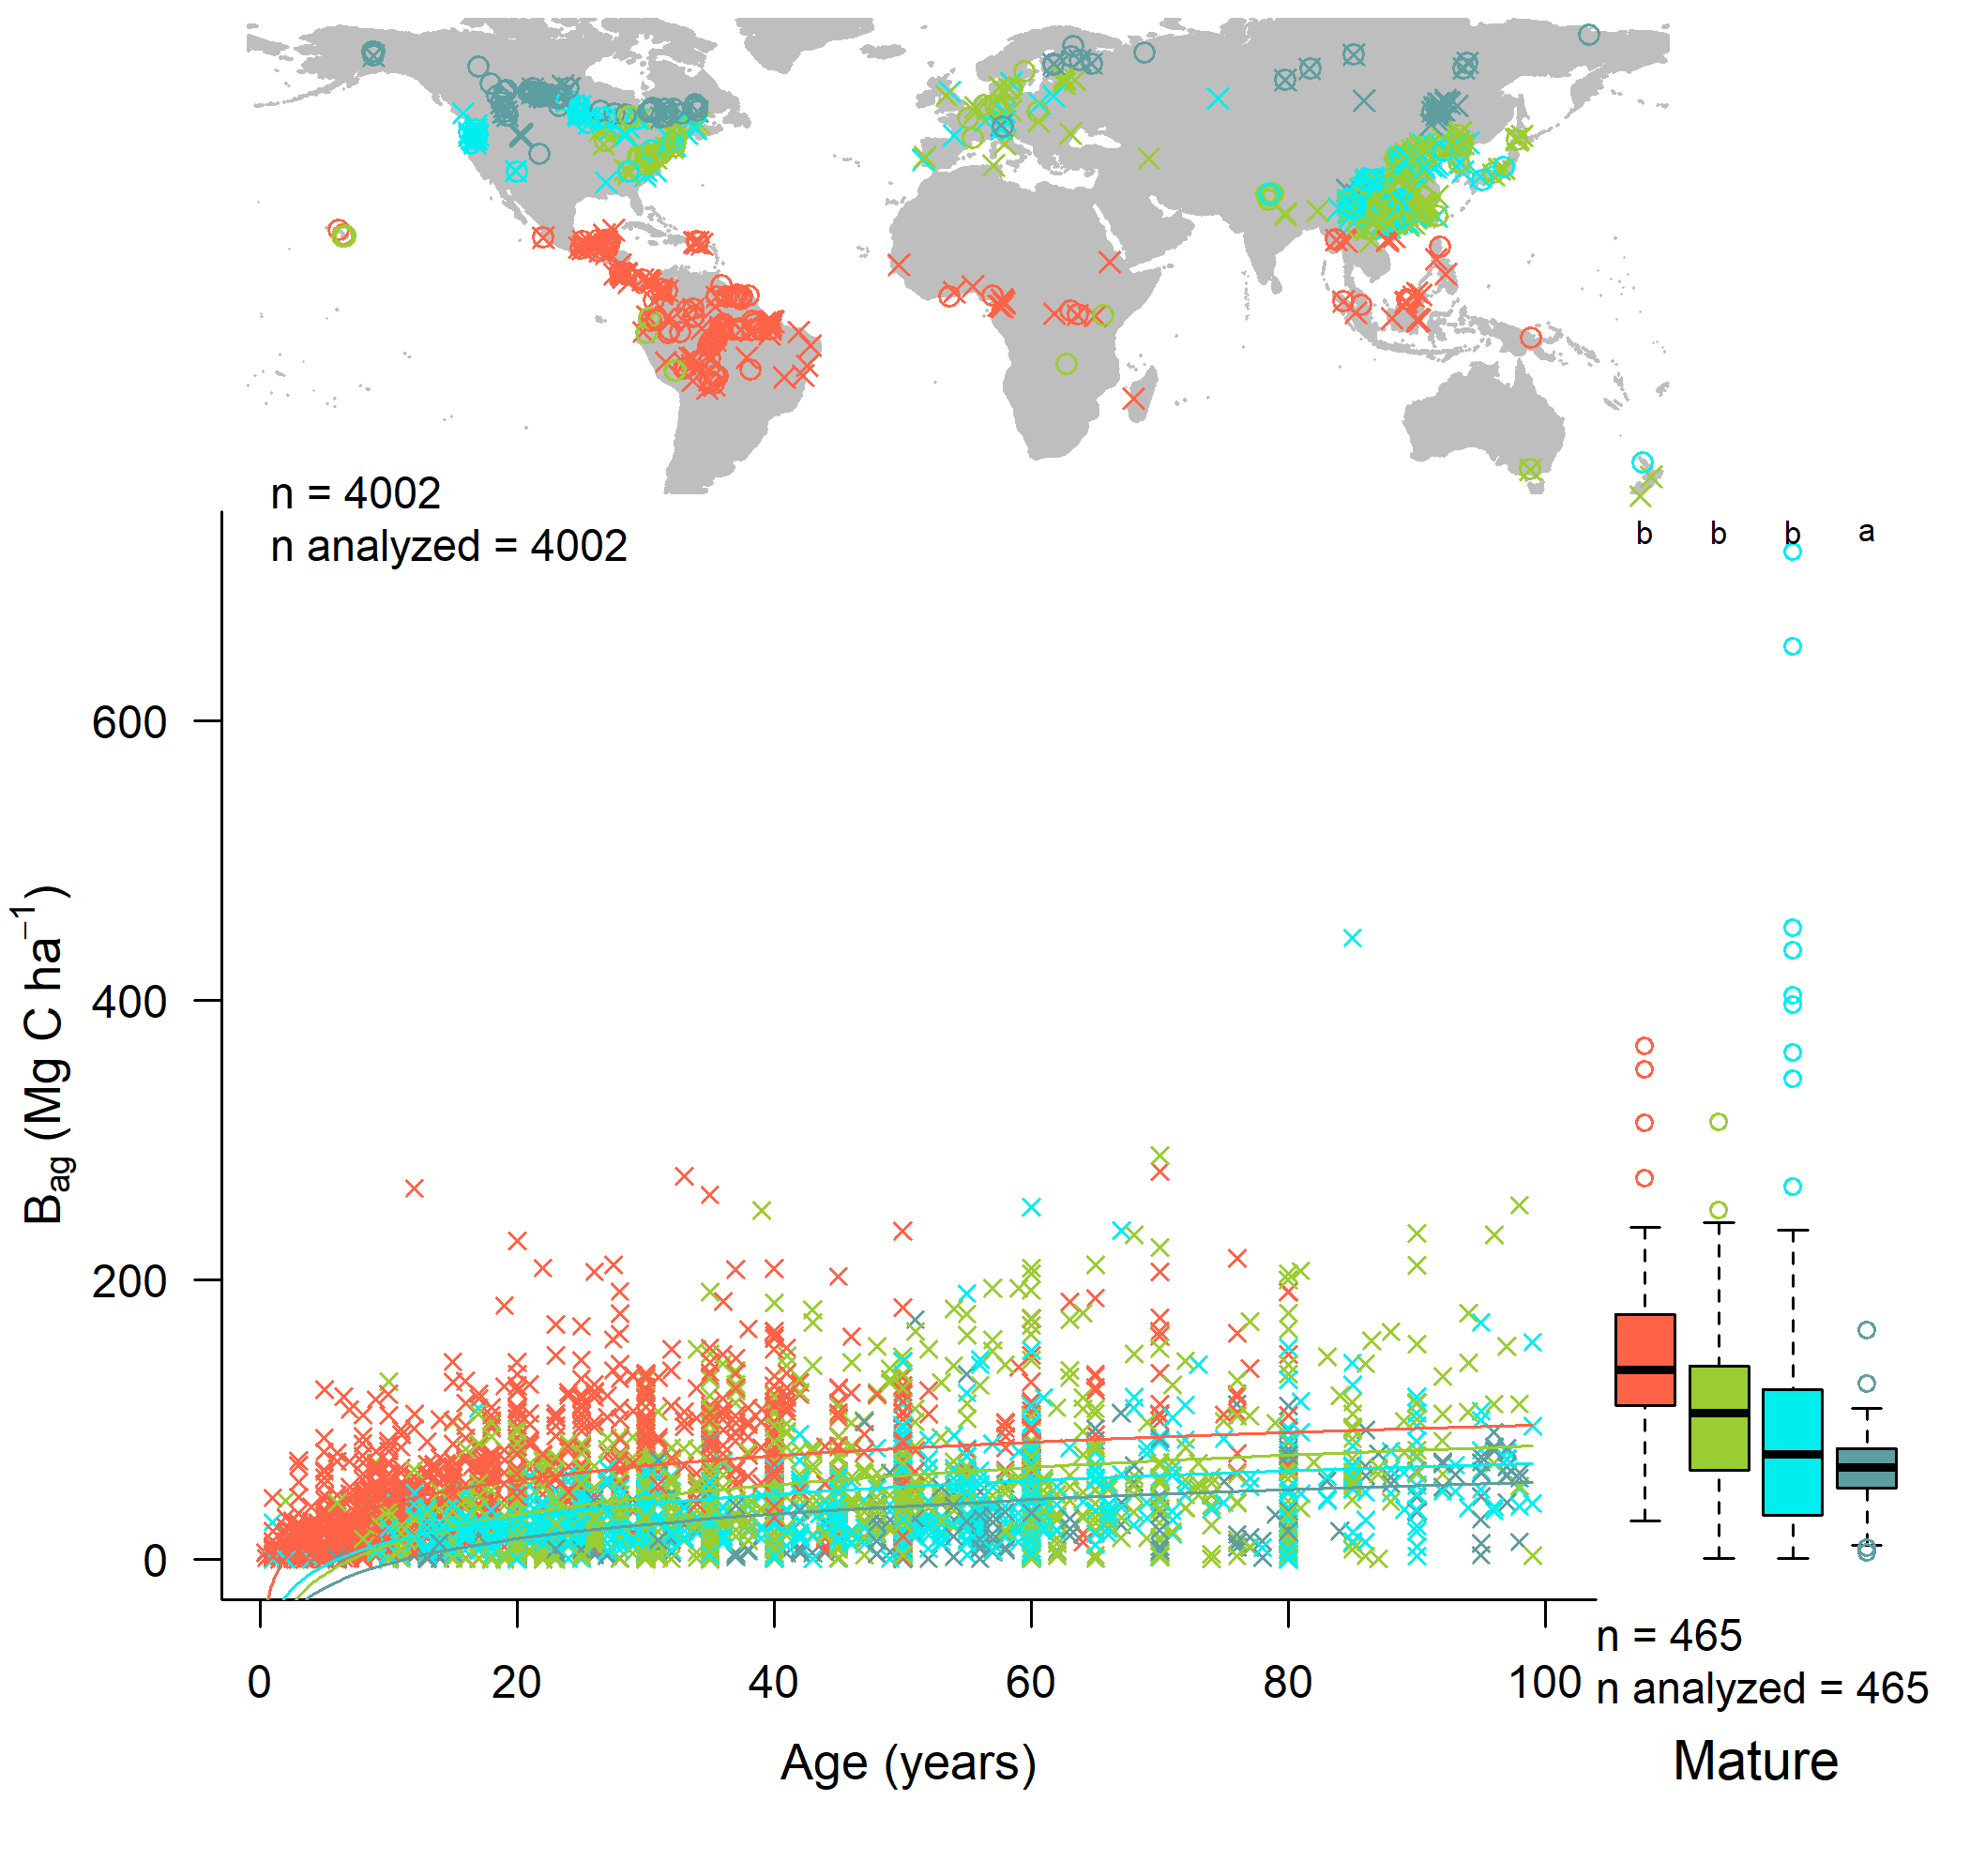
\includegraphics[width=1\linewidth]{tables_figures/age_trends/biomass_ag_with_map} 

}

\caption{Age trends and biome differences for $B_{ag}$. Map shows data sources ('$\times$' and '$\circ$' indicate young and mature stands, respectively). In each panel, the left scatterplot shows age trends in forests up to 100 years old, as characterized by a linear mixed effects model with fixed effects of log10(age) and biome. The fitted line indicates the effect of age (solid lines: significant at p<0.05, dashed lines: non-significant), and non-parallel lines indicate a significant log10(age) $\times$ biome interaction. Boxplot illustrates distribution across mature forests, with different letters indicating significant differences between biomes. Data from biomes that did not meet the sample size criteria (see Methods) are plotted, but lack regression lines (young forests) or test of differences across biomes (mature forests).}\label{fig:unnamed-chunk-24}
\end{figure}

\newpage

\hypertarget{figure-s22.-age-trends-and-biome-differences-for-b_ag-wood}{%
\subsection{\texorpdfstring{Figure S22. Age trends and biome differences
for
\(B_{ag-wood}\)}{Figure S22. Age trends and biome differences for B\_\{ag-wood\}}}\label{figure-s22.-age-trends-and-biome-differences-for-b_ag-wood}}

\begin{figure}[H]

{\centering 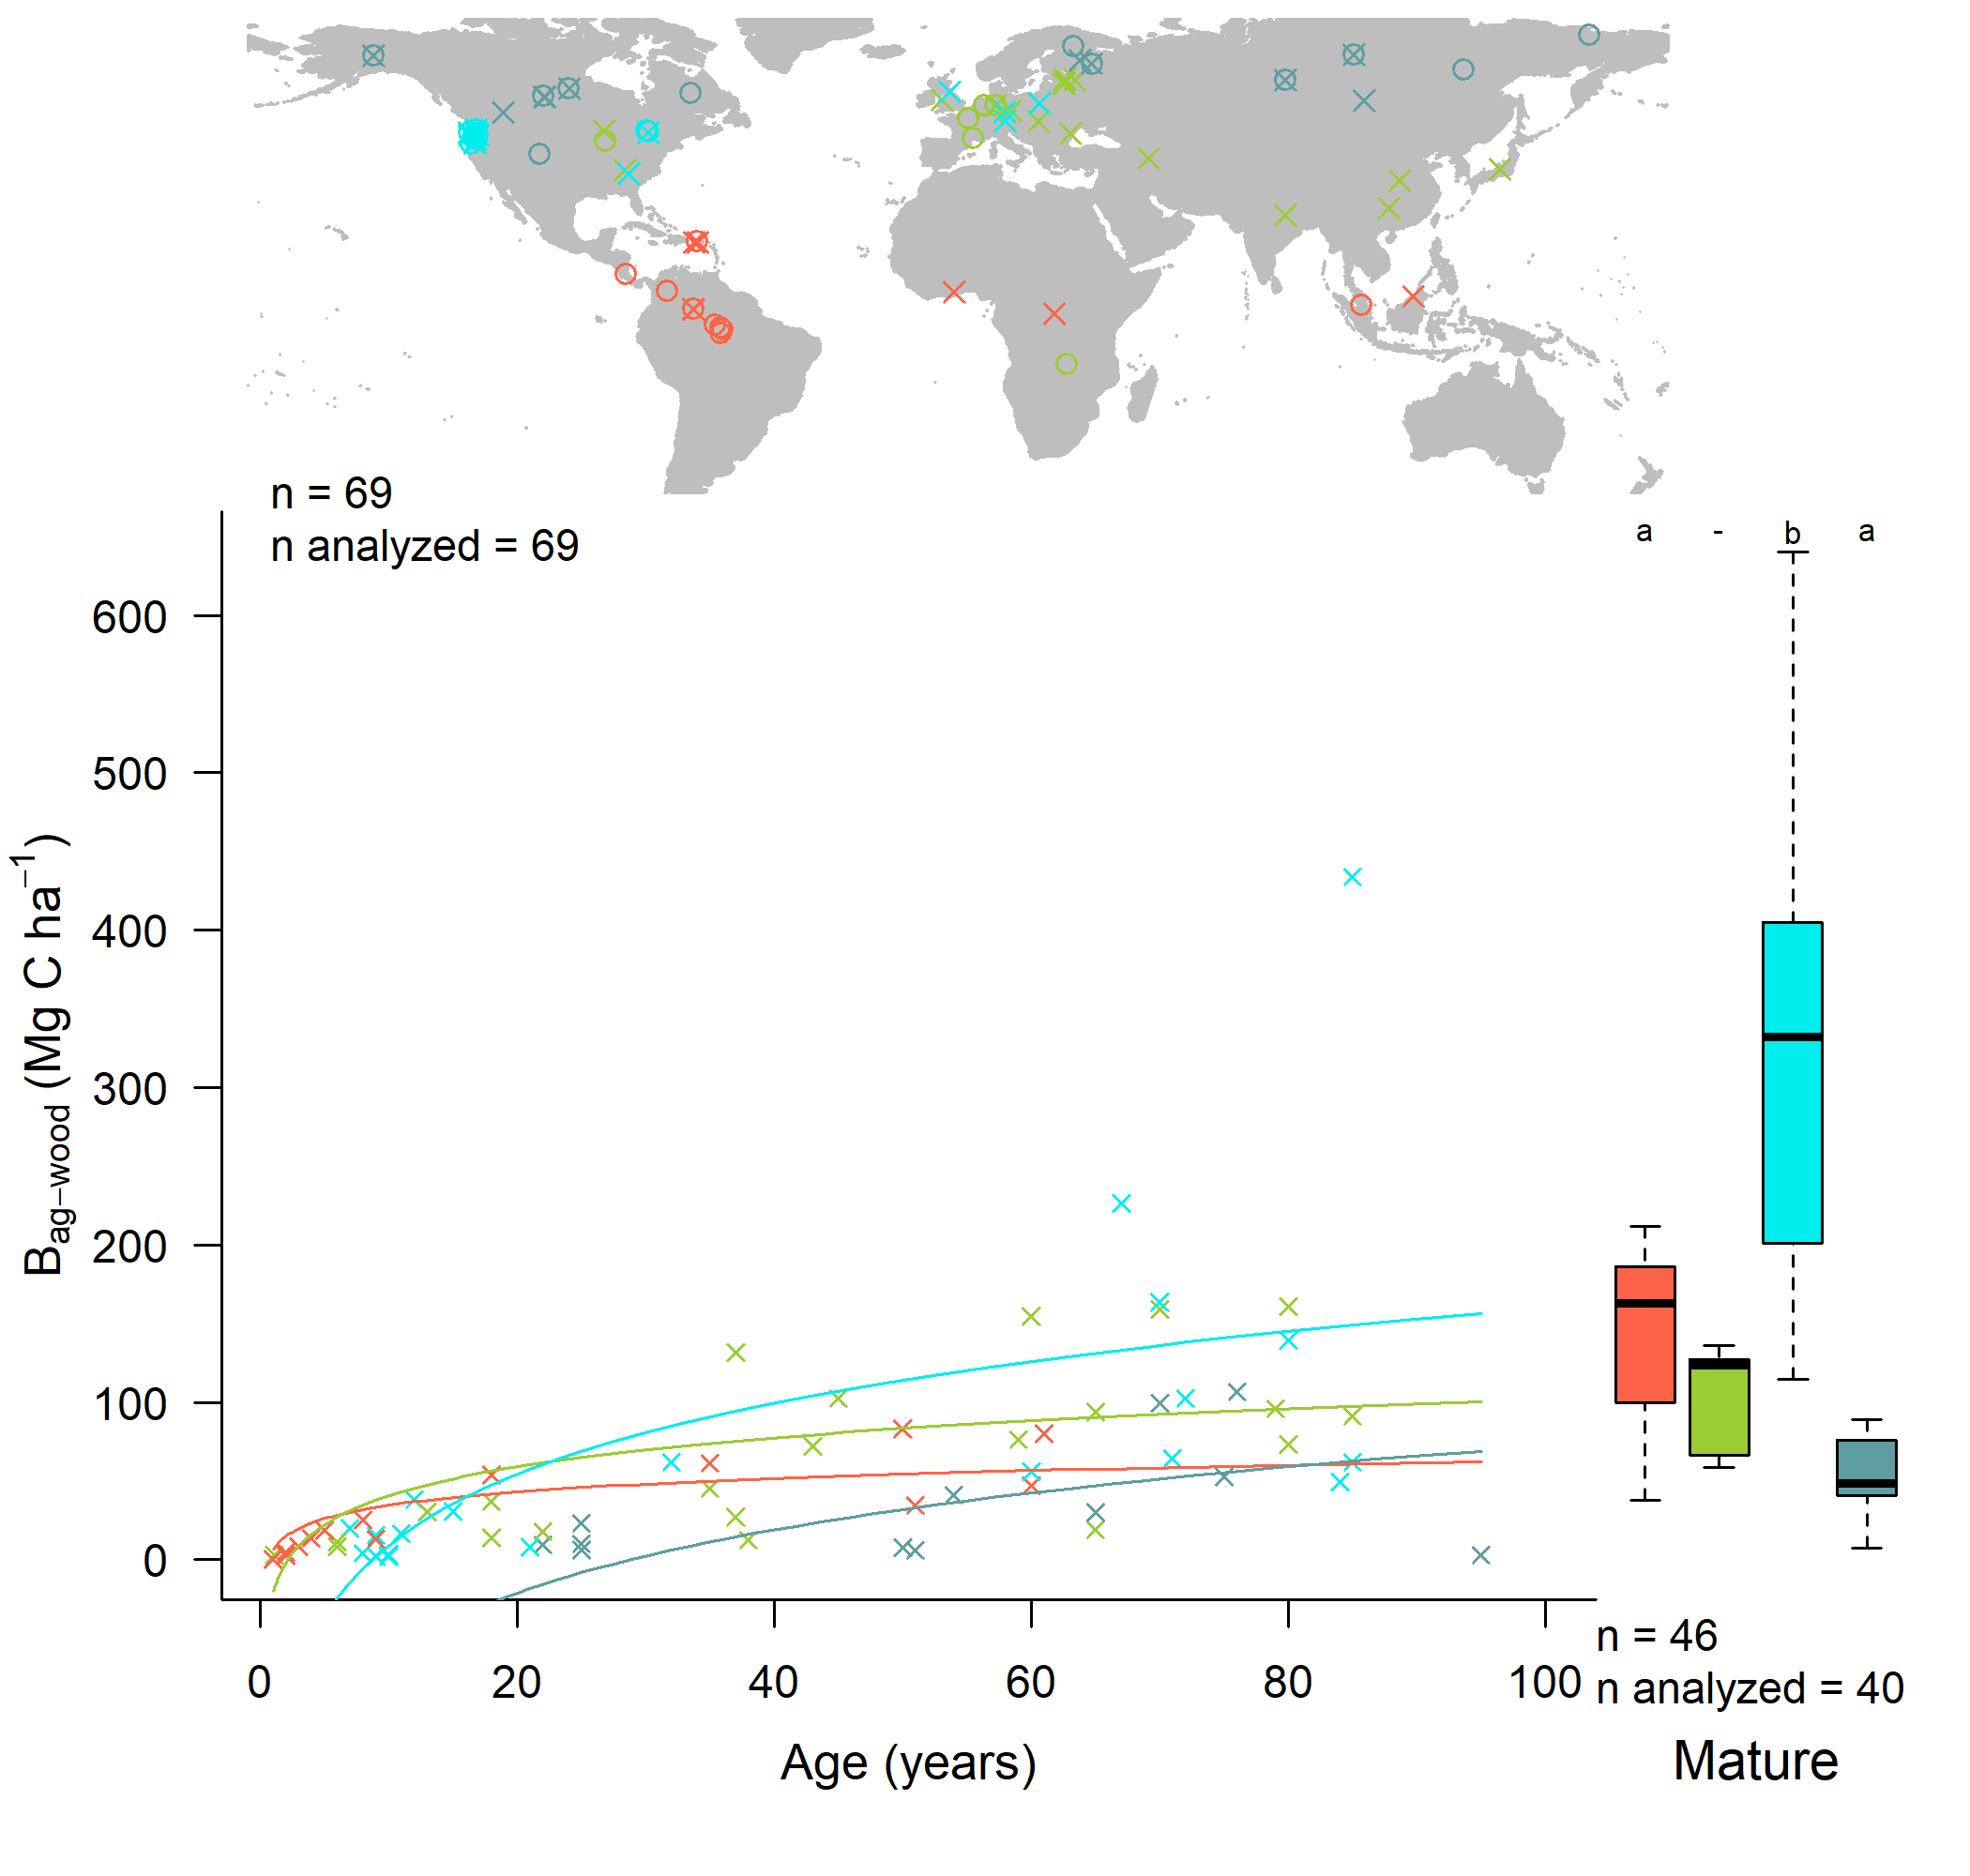
\includegraphics[width=1\linewidth]{tables_figures/age_trends/biomass_ag_woody_with_map} 

}

\caption{Age trends and biome differences for $B_{ag-wood}$. Map shows data sources ('$\times$' and '$\circ$' indicate young and mature stands, respectively). In each panel, the left scatterplot shows age trends in forests up to 100 years old, as characterized by a linear mixed effects model with fixed effects of log10(age) and biome. The fitted line indicates the effect of age (solid lines: significant at p<0.05, dashed lines: non-significant), and non-parallel lines indicate a significant log10(age) $\times$ biome interaction. Boxplot illustrates distribution across mature forests, with different letters indicating significant differences between biomes. Data from biomes that did not meet the sample size criteria (see Methods) are plotted, but lack regression lines (young forests) or test of differences across biomes (mature forests).}\label{fig:unnamed-chunk-25}
\end{figure}

\newpage

\hypertarget{figure-s23.-age-trends-and-biome-differences-for-b_foliage}{%
\subsection{\texorpdfstring{Figure S23. Age trends and biome differences
for
\(B_{foliage}\)}{Figure S23. Age trends and biome differences for B\_\{foliage\}}}\label{figure-s23.-age-trends-and-biome-differences-for-b_foliage}}

\begin{figure}[H]

{\centering 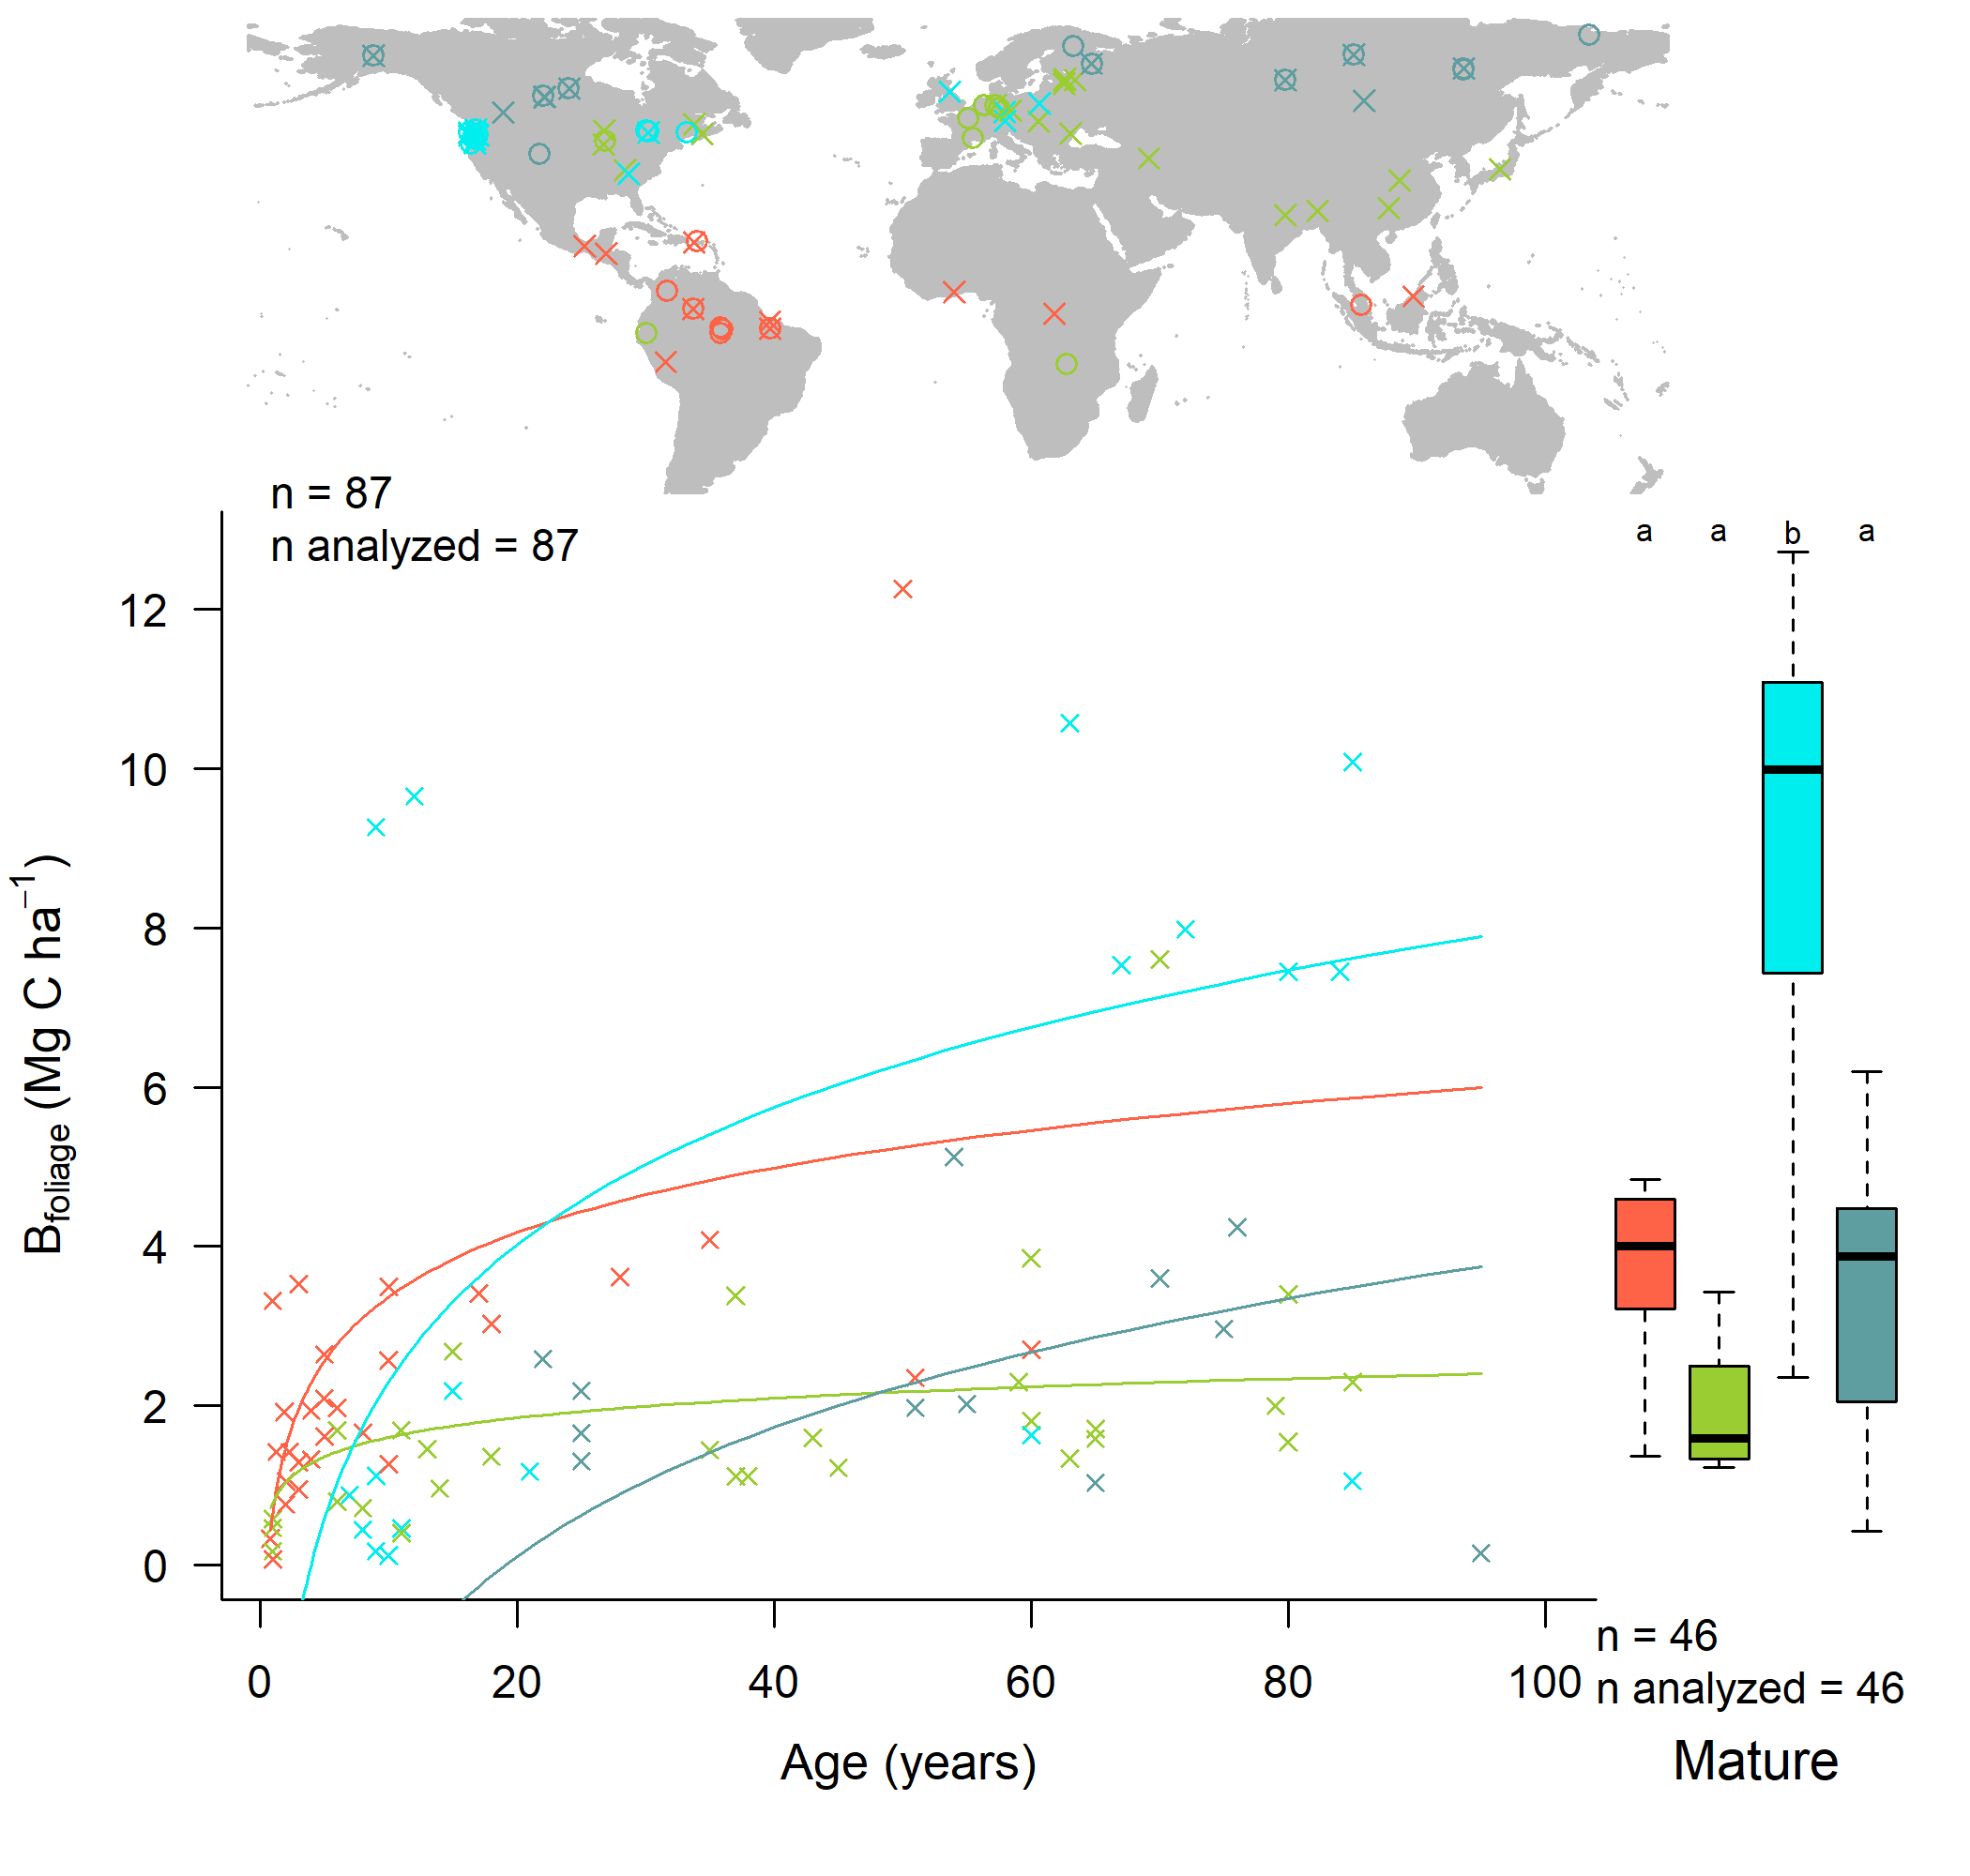
\includegraphics[width=1\linewidth]{tables_figures/age_trends/biomass_foliage_with_map} 

}

\caption{Age trends and biome differences for $B_{foliage}$. Map shows data sources ('$\times$' and '$\circ$' indicate young and mature stands, respectively). In each panel, the left scatterplot shows age trends in forests up to 100 years old, as characterized by a linear mixed effects model with fixed effects of log10(age) and biome. The fitted line indicates the effect of age (solid lines: significant at p<0.05, dashed lines: non-significant), and non-parallel lines indicate a significant log10(age) $\times$ biome interaction. Boxplot illustrates distribution across mature forests, with different letters indicating significant differences between biomes. Data from biomes that did not meet the sample size criteria (see Methods) are plotted, but lack regression lines (young forests) or test of differences across biomes (mature forests).}\label{fig:unnamed-chunk-26}
\end{figure}

\newpage

\hypertarget{figure-s24.-age-trends-and-biome-differences-for-b_root}{%
\subsection{\texorpdfstring{Figure S24. Age trends and biome differences
for
\(B_{root}\)}{Figure S24. Age trends and biome differences for B\_\{root\}}}\label{figure-s24.-age-trends-and-biome-differences-for-b_root}}

\begin{figure}[H]

{\centering 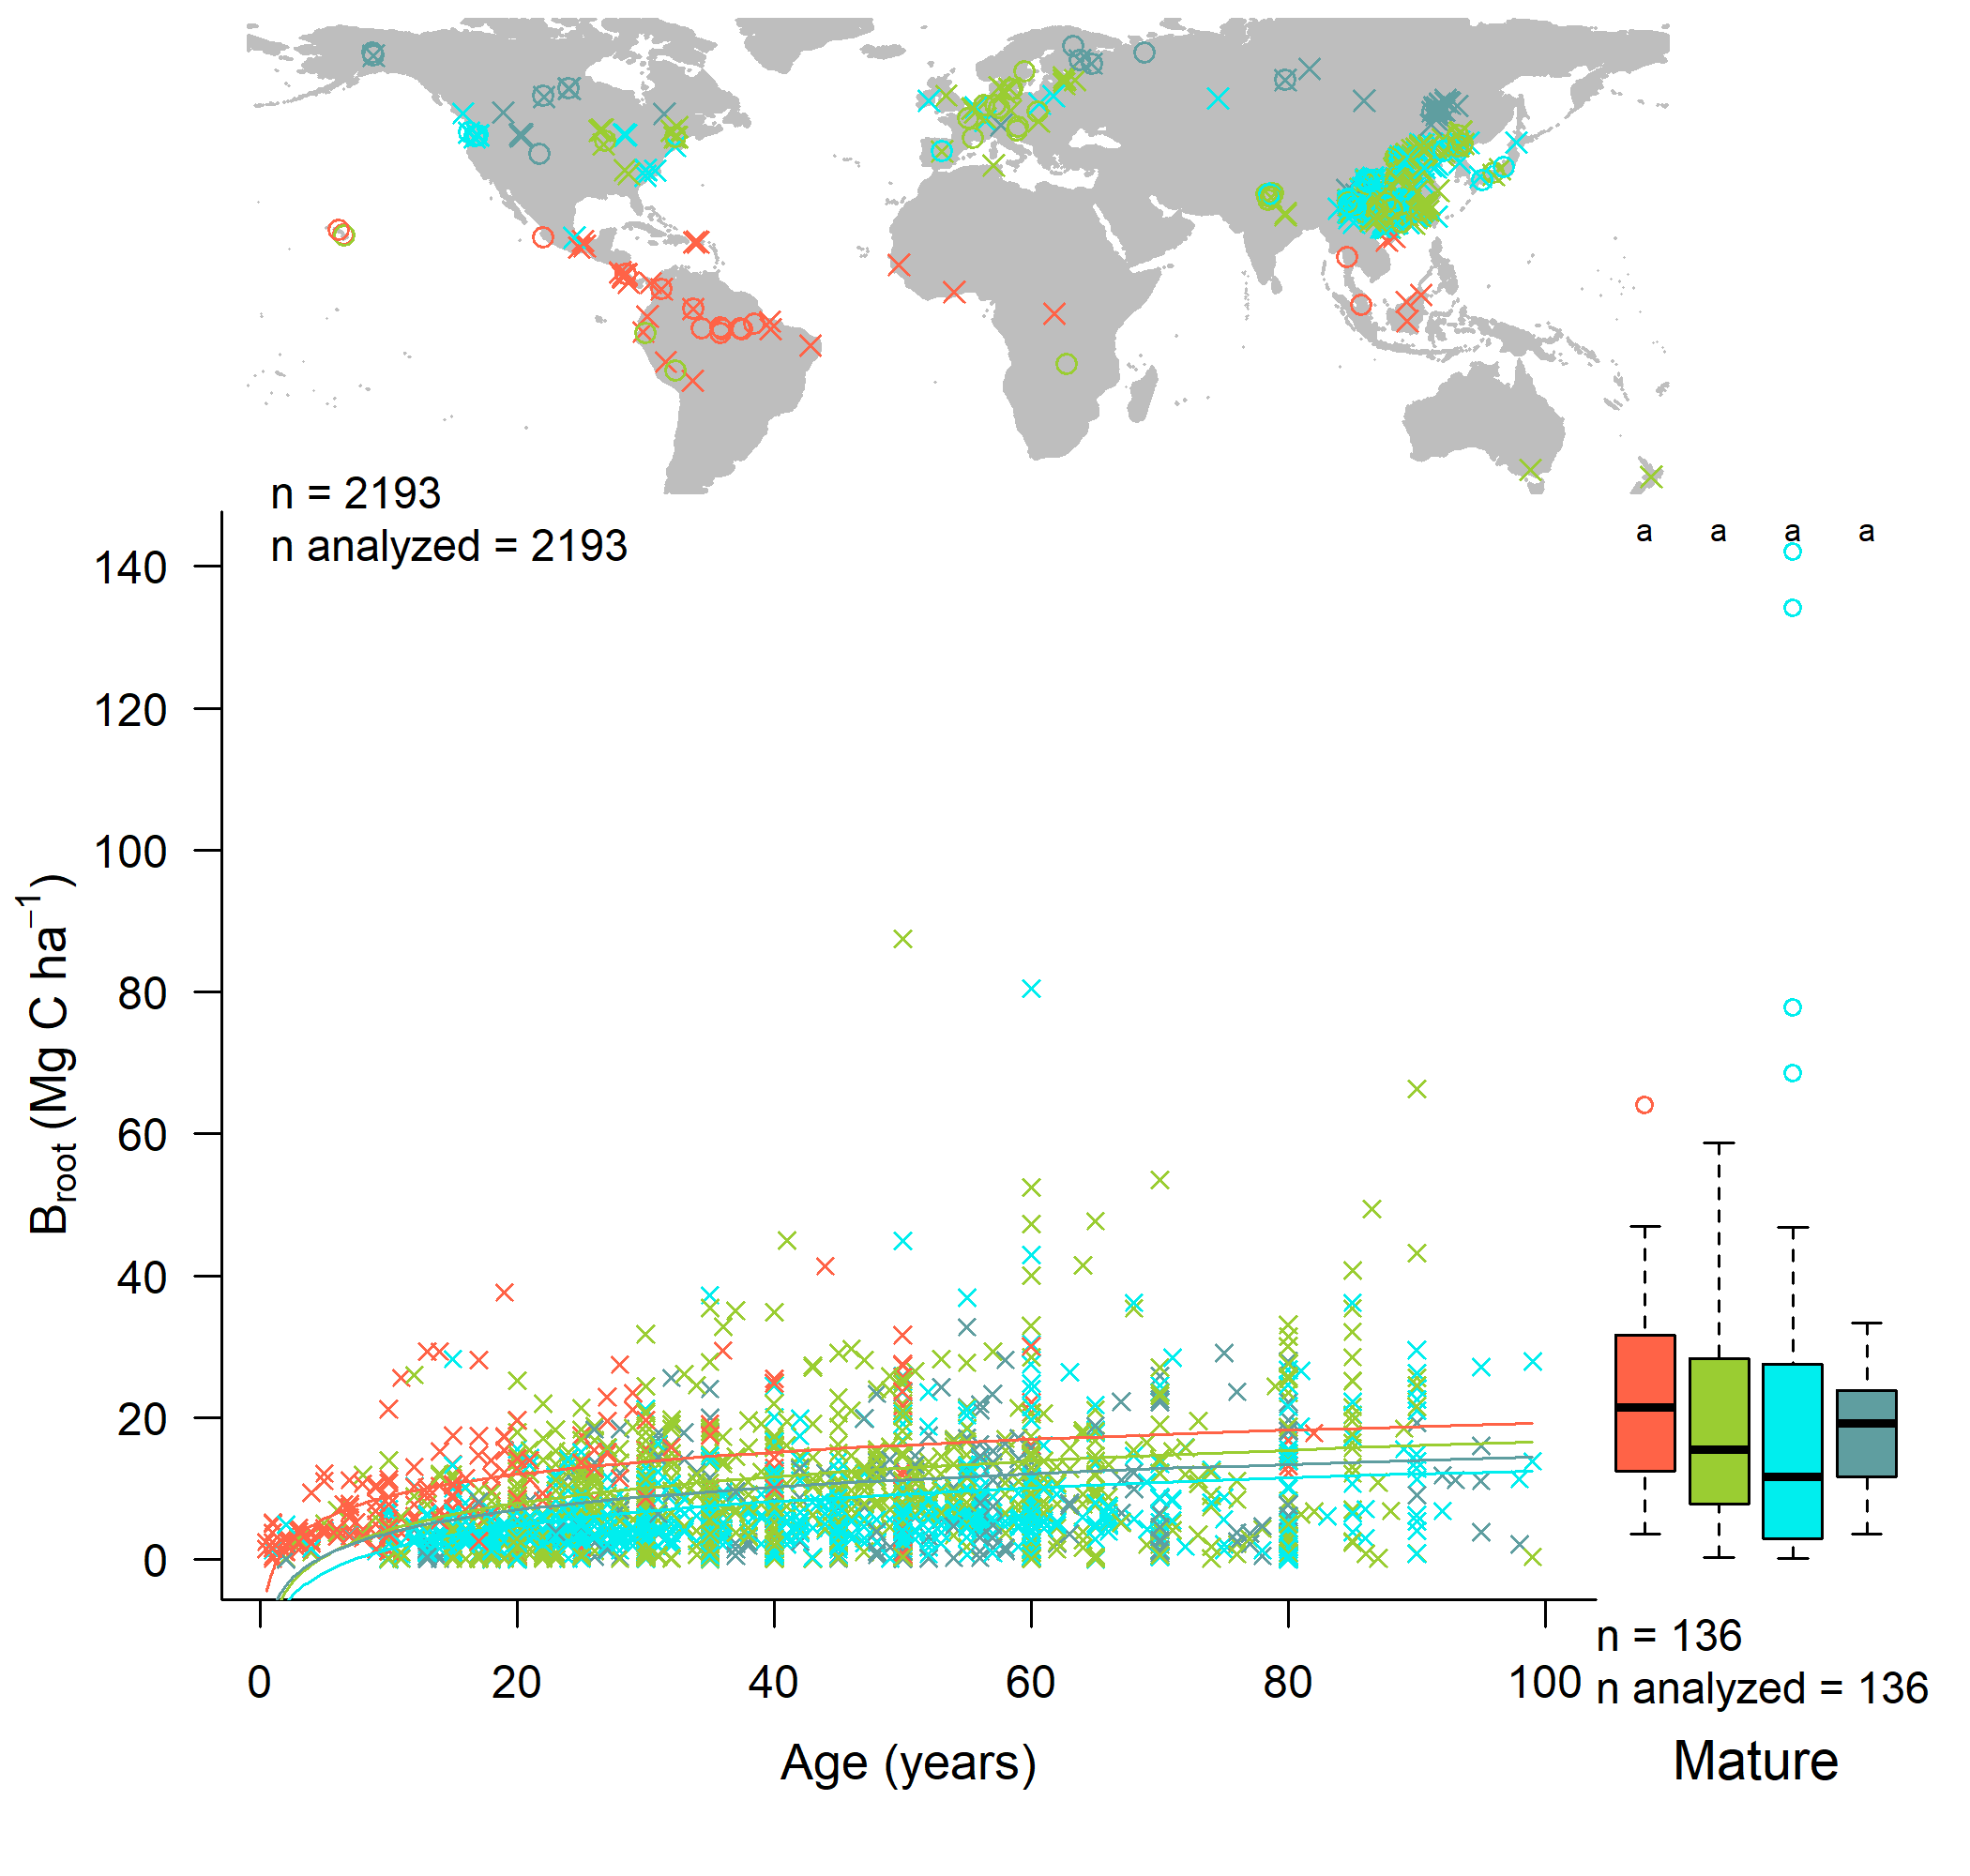
\includegraphics[width=1\linewidth]{tables_figures/age_trends/biomass_root_with_map} 

}

\caption{Age trends and biome differences for $B_{root}$. Map shows data sources ('$\times$' and '$\circ$' indicate young and mature stands, respectively). In each panel, the left scatterplot shows age trends in forests up to 100 years old, as characterized by a linear mixed effects model with fixed effects of log10(age) and biome. The fitted line indicates the effect of age (solid lines: significant at p<0.05, dashed lines: non-significant), and non-parallel lines indicate a significant log10(age) $\times$ biome interaction. Boxplot illustrates distribution across mature forests, with different letters indicating significant differences between biomes. Data from biomes that did not meet the sample size criteria (see Methods) are plotted, but lack regression lines (young forests) or test of differences across biomes (mature forests).}\label{fig:unnamed-chunk-27}
\end{figure}

\newpage

\hypertarget{figure-s25.-age-trends-and-biome-differences-for-b_root-coarse}{%
\subsection{\texorpdfstring{Figure S25. Age trends and biome differences
for
\(B_{root-coarse}\)}{Figure S25. Age trends and biome differences for B\_\{root-coarse\}}}\label{figure-s25.-age-trends-and-biome-differences-for-b_root-coarse}}

\begin{figure}[H]

{\centering 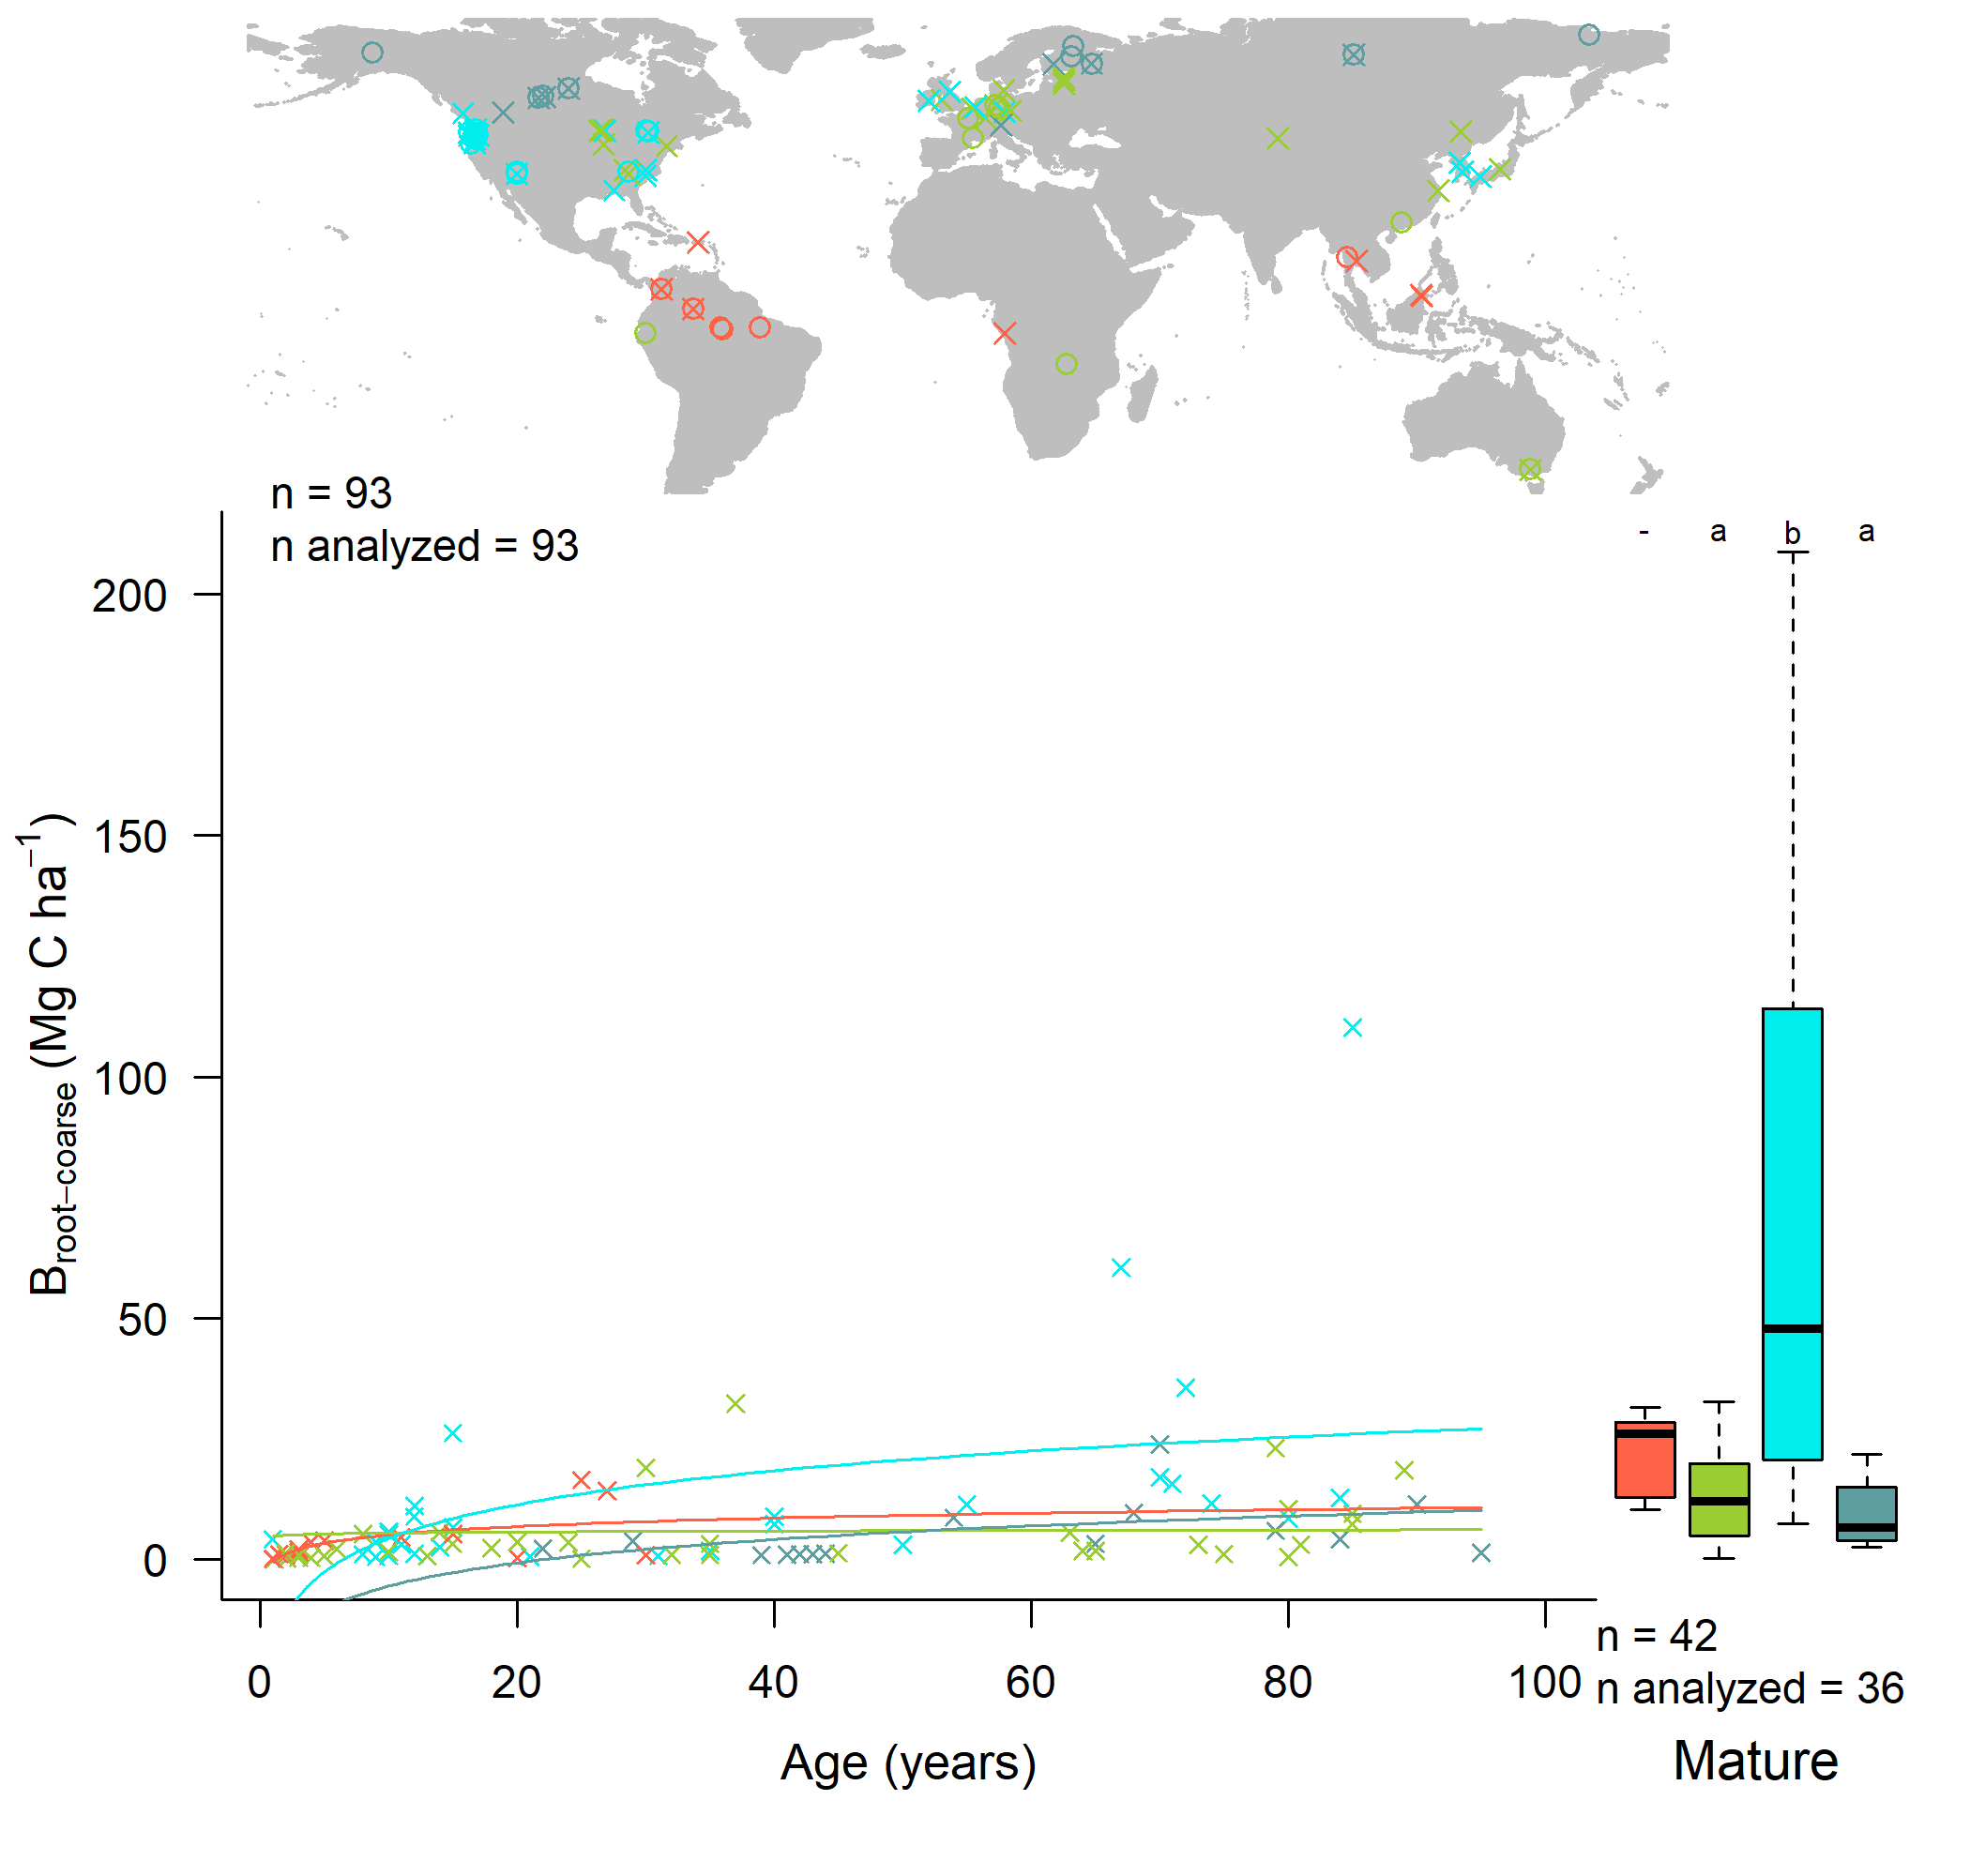
\includegraphics[width=1\linewidth]{tables_figures/age_trends/biomass_root_coarse_with_map} 

}

\caption{Age trends and biome differences for $B_{root-coarse}$. Map shows data sources ('$\times$' and '$\circ$' indicate young and mature stands, respectively). In each panel, the left scatterplot shows age trends in forests up to 100 years old, as characterized by a linear mixed effects model with fixed effects of log10(age) and biome. The fitted line indicates the effect of age (solid lines: significant at p<0.05, dashed lines: non-significant), and non-parallel lines indicate a significant log10(age) $\times$ biome interaction. Boxplot illustrates distribution across mature forests, with different letters indicating significant differences between biomes. Data from biomes that did not meet the sample size criteria (see Methods) are plotted, but lack regression lines (young forests) or test of differences across biomes (mature forests).}\label{fig:unnamed-chunk-28}
\end{figure}

\newpage

\hypertarget{figure-s26.-age-trends-and-biome-differences-for-b_root-fine}{%
\subsection{\texorpdfstring{Figure S26. Age trends and biome differences
for
\(B_{root-fine}\)}{Figure S26. Age trends and biome differences for B\_\{root-fine\}}}\label{figure-s26.-age-trends-and-biome-differences-for-b_root-fine}}

\begin{figure}[H]

{\centering 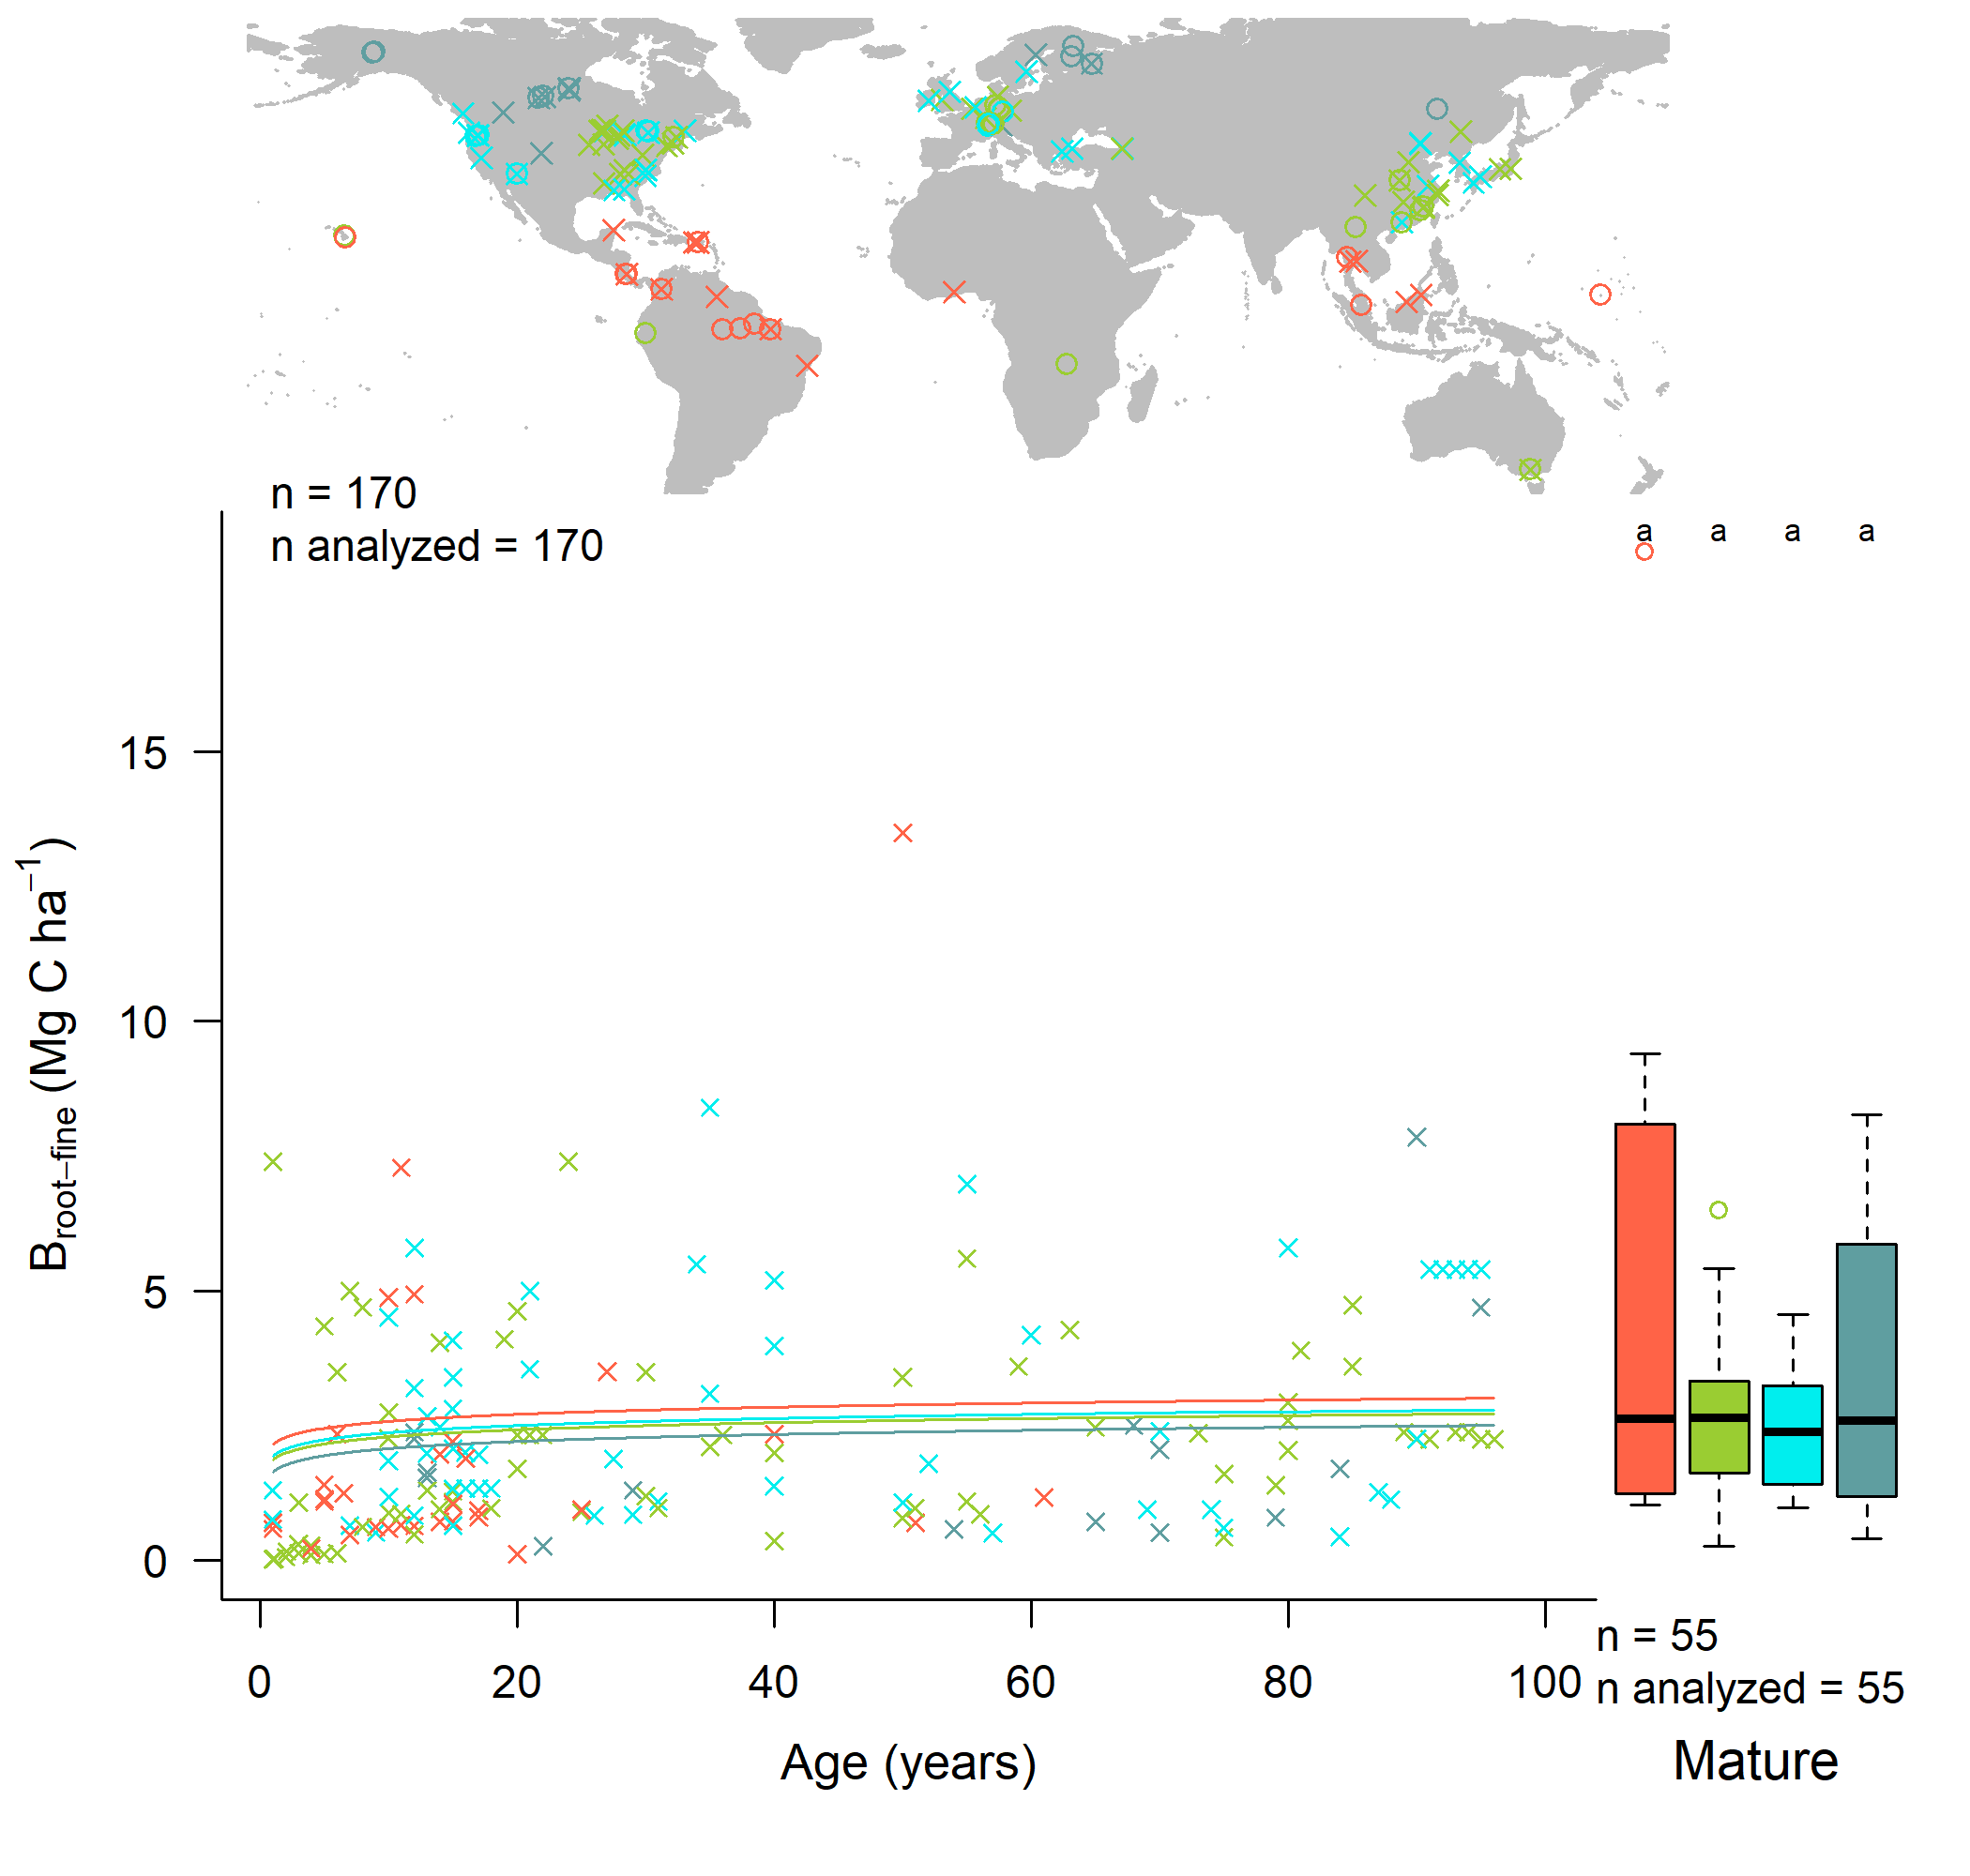
\includegraphics[width=1\linewidth]{tables_figures/age_trends/biomass_root_fine_with_map} 

}

\caption{Age trends and biome differences for $B_{root-fine}$. Map shows data sources ('$\times$' and '$\circ$' indicate young and mature stands, respectively). In each panel, the left scatterplot shows age trends in forests up to 100 years old, as characterized by a linear mixed effects model with fixed effects of log10(age) and biome. The fitted line indicates the effect of age (solid lines: significant at p<0.05, dashed lines: non-significant), and non-parallel lines indicate a significant log10(age) $\times$ biome interaction. Boxplot illustrates distribution across mature forests, with different letters indicating significant differences between biomes. Data from biomes that did not meet the sample size criteria (see Methods) are plotted, but lack regression lines (young forests) or test of differences across biomes (mature forests).}\label{fig:unnamed-chunk-29}
\end{figure}

\newpage

\hypertarget{figure-s27.-age-trends-and-biome-differences-for-dw_tot}{%
\subsection{\texorpdfstring{Figure S27. Age trends and biome differences
for
\(DW_{tot}\)}{Figure S27. Age trends and biome differences for DW\_\{tot\}}}\label{figure-s27.-age-trends-and-biome-differences-for-dw_tot}}

\begin{figure}[H]

{\centering 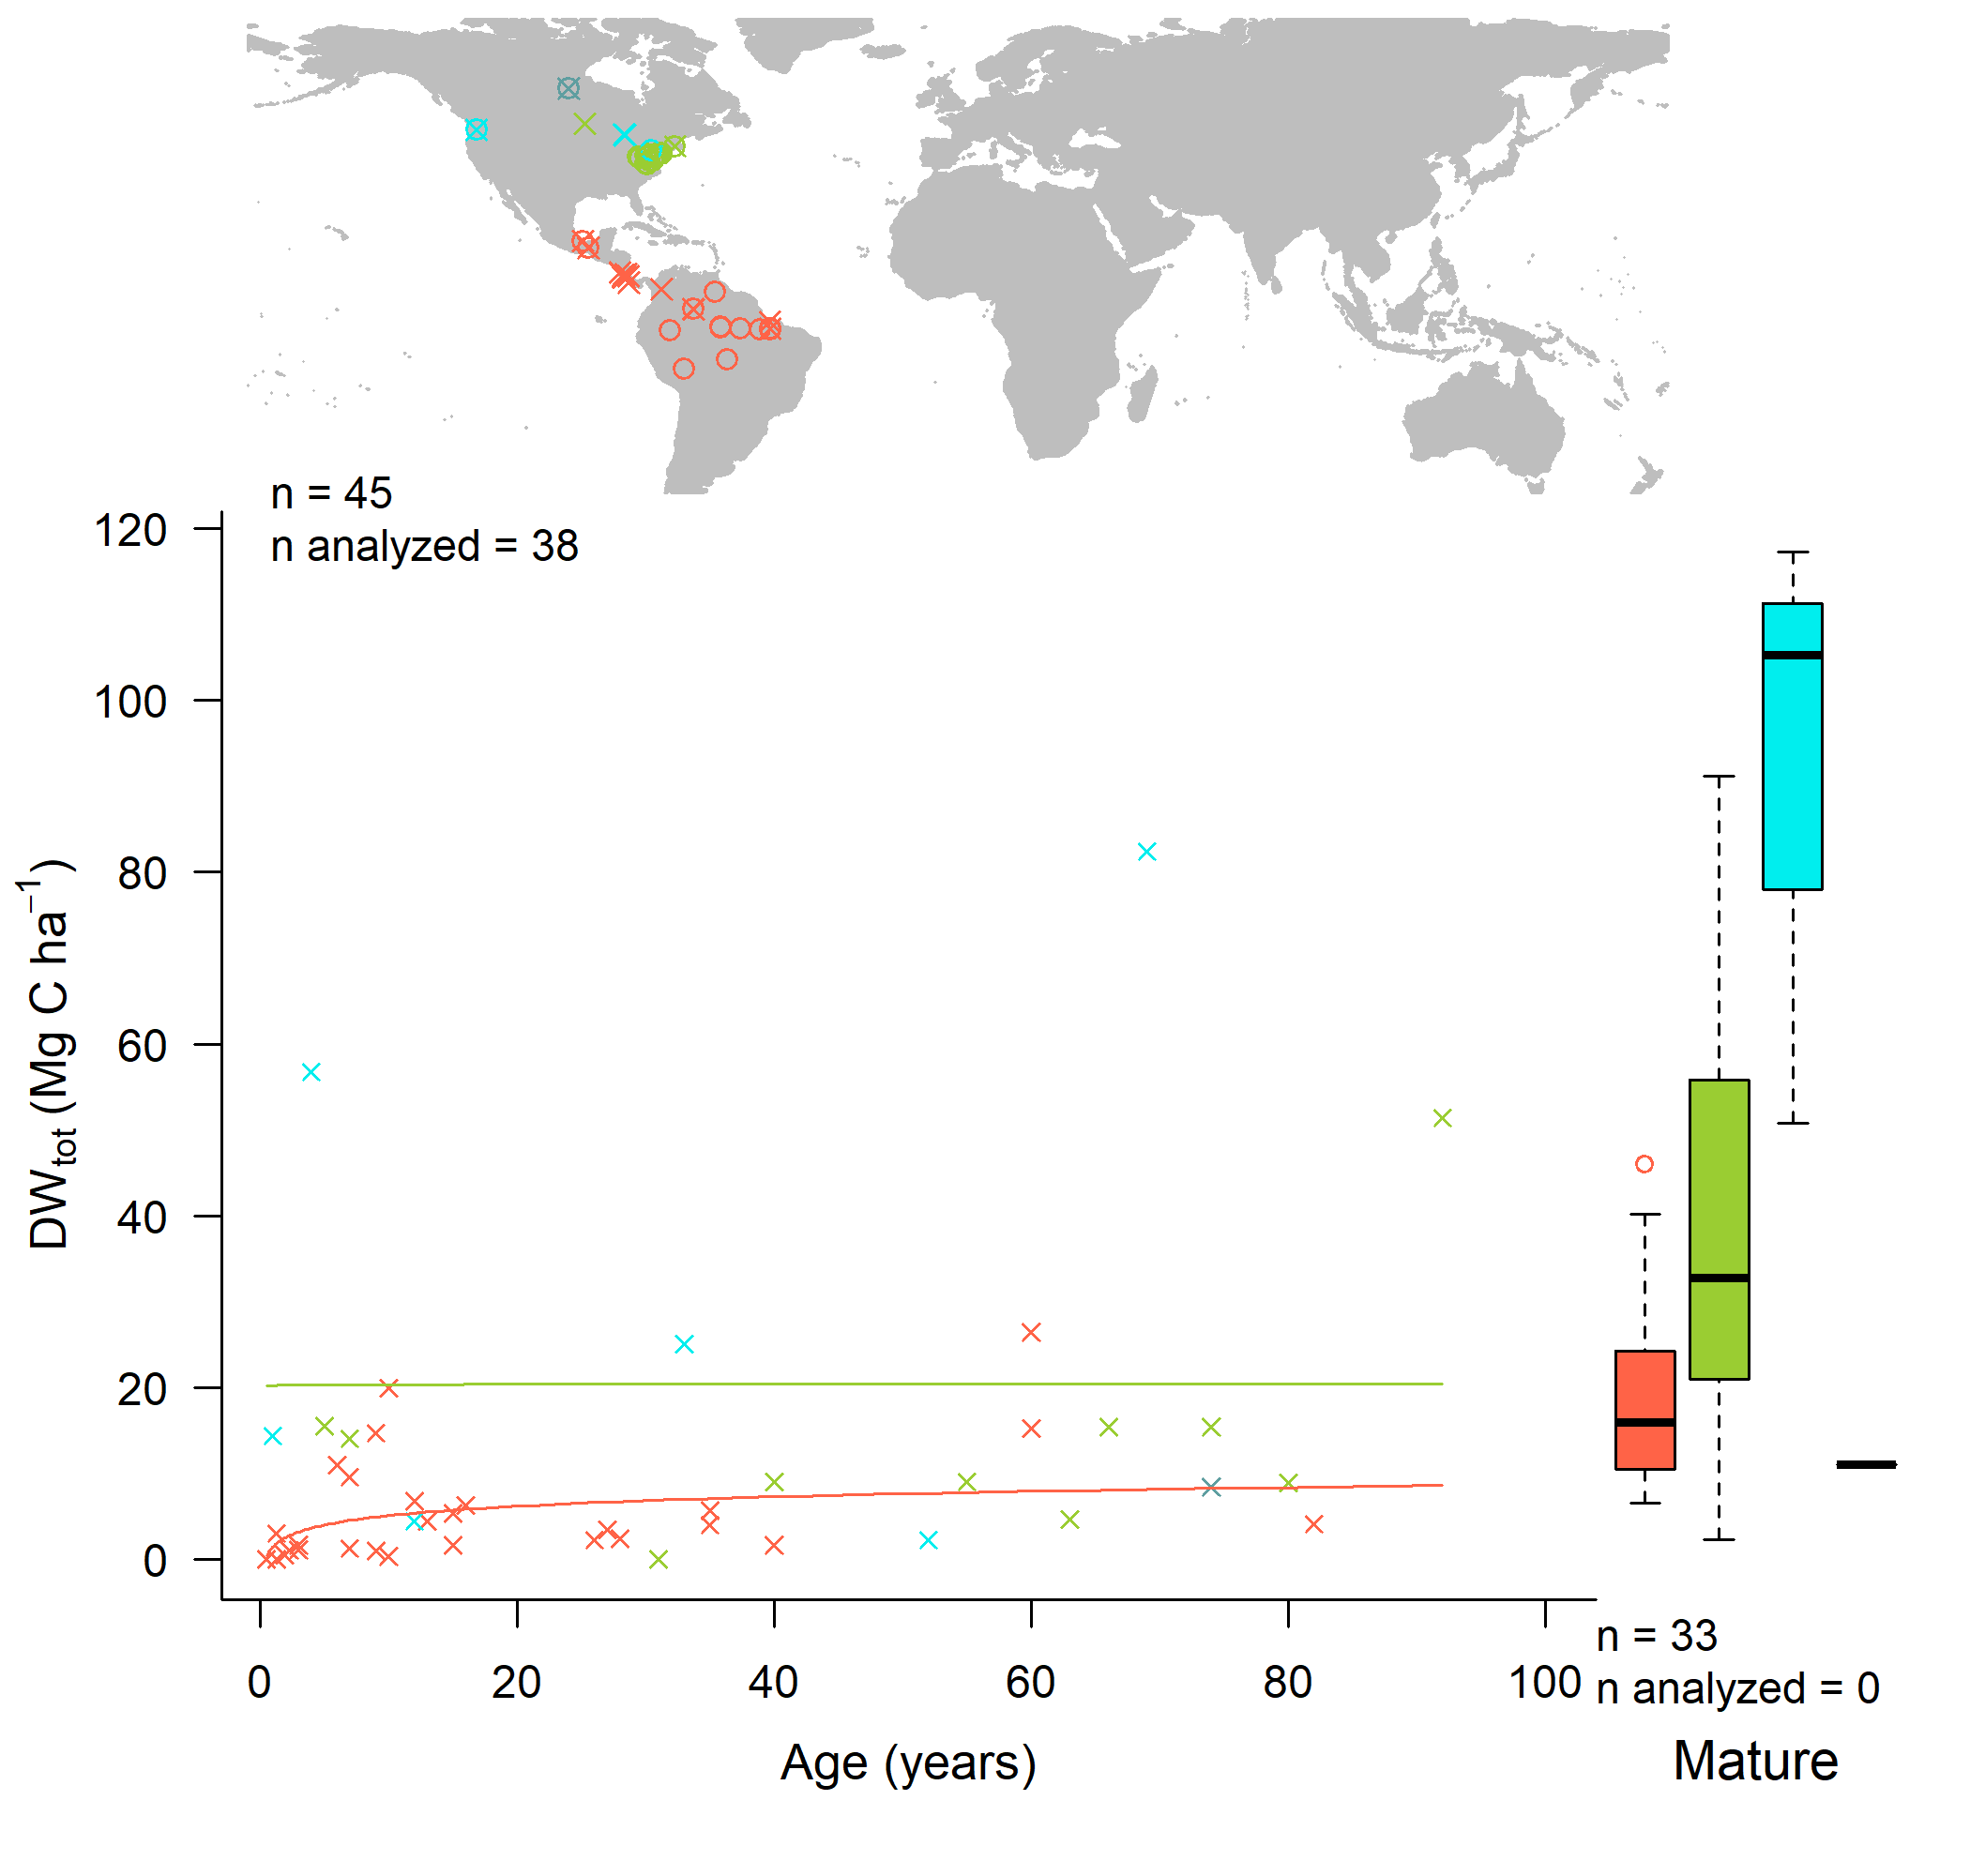
\includegraphics[width=1\linewidth]{tables_figures/age_trends/deadwood_with_map} 

}

\caption{Age trends and biome differences for $DW_{tot}$. Map shows data sources ('$\times$' and '$\circ$' indicate young and mature stands, respectively). In each panel, the left scatterplot shows age trends in forests up to 100 years old, as characterized by a linear mixed effects model with fixed effects of log10(age) and biome. The fitted line indicates the effect of age (solid lines: significant at p<0.05, dashed lines: non-significant), and non-parallel lines indicate a significant log10(age) $\times$ biome interaction. Boxplot illustrates distribution across mature forests, with different letters indicating significant differences between biomes. Data from biomes that did not meet the sample size criteria (see Methods) are plotted, but lack regression lines (young forests) or test of differences across biomes (mature forests).}\label{fig:unnamed-chunk-30}
\end{figure}

\newpage

\hypertarget{figure-s28.-age-trends-and-biome-differences-for-dw_standing}{%
\subsection{\texorpdfstring{Figure S28. Age trends and biome differences
for
\(DW_{standing}\)}{Figure S28. Age trends and biome differences for DW\_\{standing\}}}\label{figure-s28.-age-trends-and-biome-differences-for-dw_standing}}

\begin{figure}[H]

{\centering 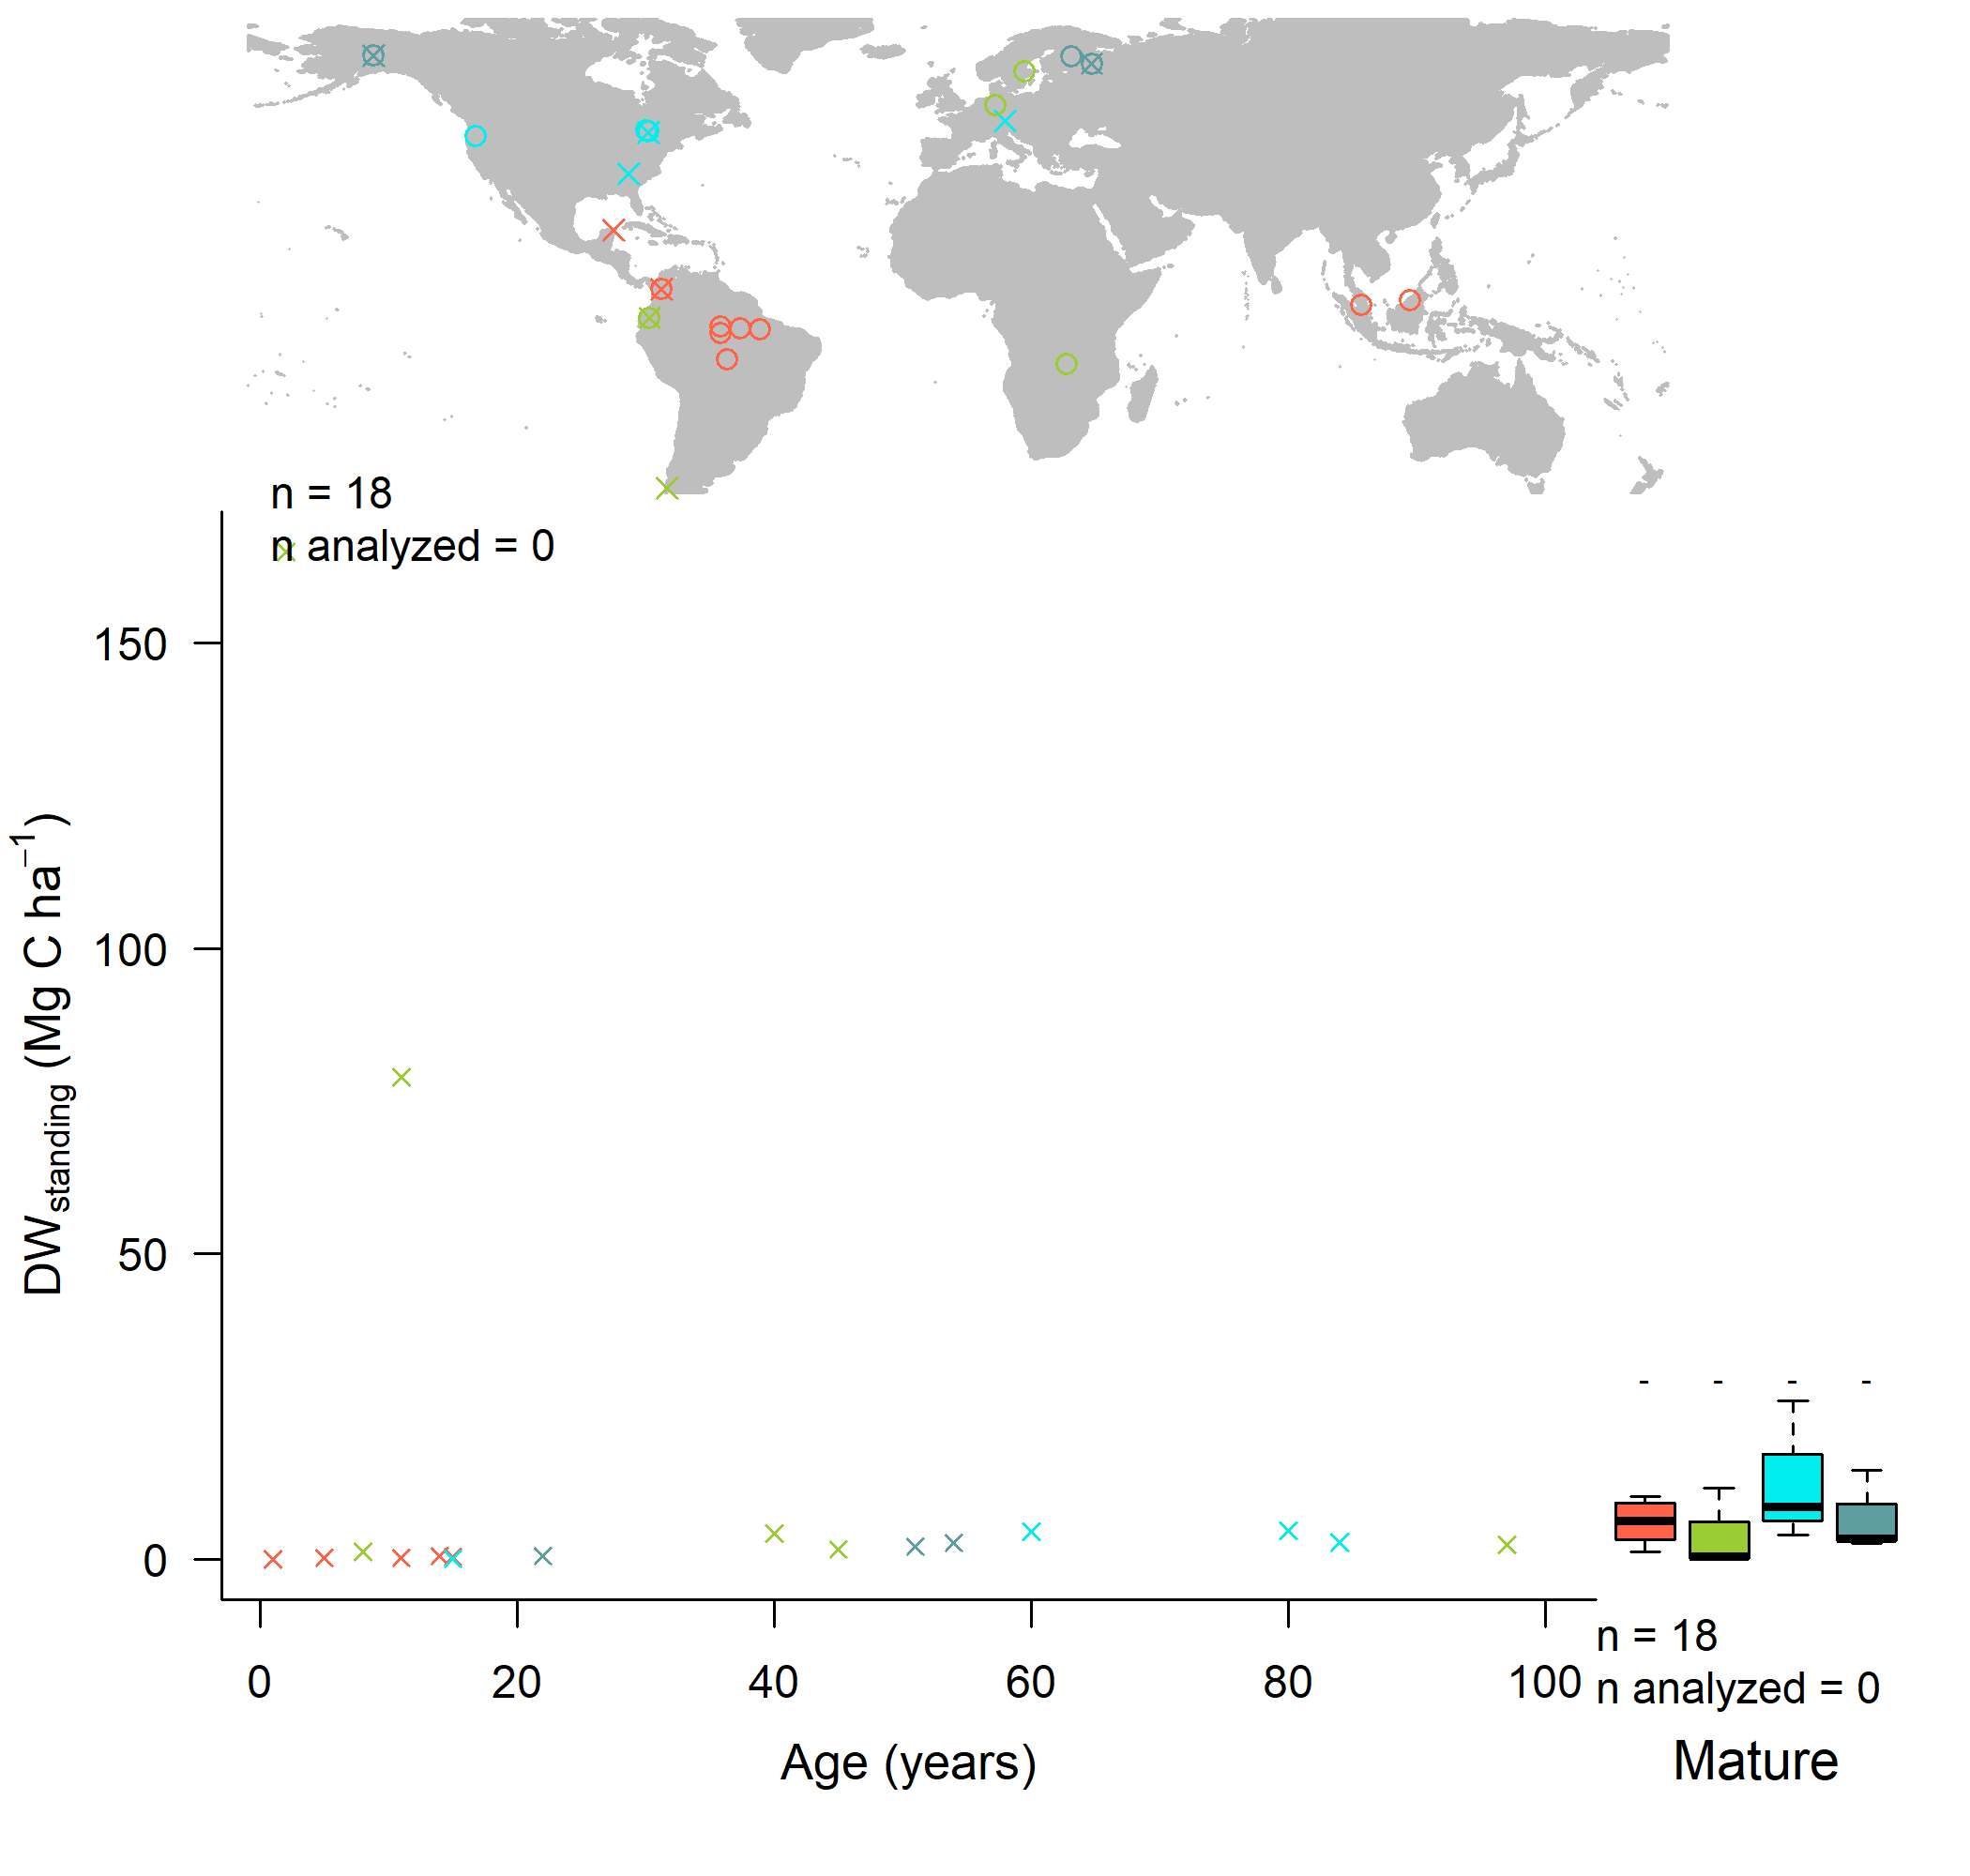
\includegraphics[width=1\linewidth]{tables_figures/age_trends/deadwood_standing_with_map} 

}

\caption{Age trends and biome differences for $DW_{standing}$. Map shows data sources ('$\times$' and '$\circ$' indicate young and mature stands, respectively). In each panel, the left scatterplot shows age trends in forests up to 100 years old, as characterized by a linear mixed effects model with fixed effects of log10(age) and biome. The fitted line indicates the effect of age (solid lines: significant at p<0.05, dashed lines: non-significant), and non-parallel lines indicate a significant log10(age) $\times$ biome interaction. Boxplot illustrates distribution across mature forests, with different letters indicating significant differences between biomes. Data from biomes that did not meet the sample size criteria (see Methods) are plotted, but lack regression lines (young forests) or test of differences across biomes (mature forests).}\label{fig:unnamed-chunk-31}
\end{figure}

\newpage

\hypertarget{figure-s29.-age-trends-and-biome-differences-for-dw_down}{%
\subsection{\texorpdfstring{Figure S29. Age trends and biome differences
for
\(DW_{down}\)}{Figure S29. Age trends and biome differences for DW\_\{down\}}}\label{figure-s29.-age-trends-and-biome-differences-for-dw_down}}

\begin{figure}[H]

{\centering 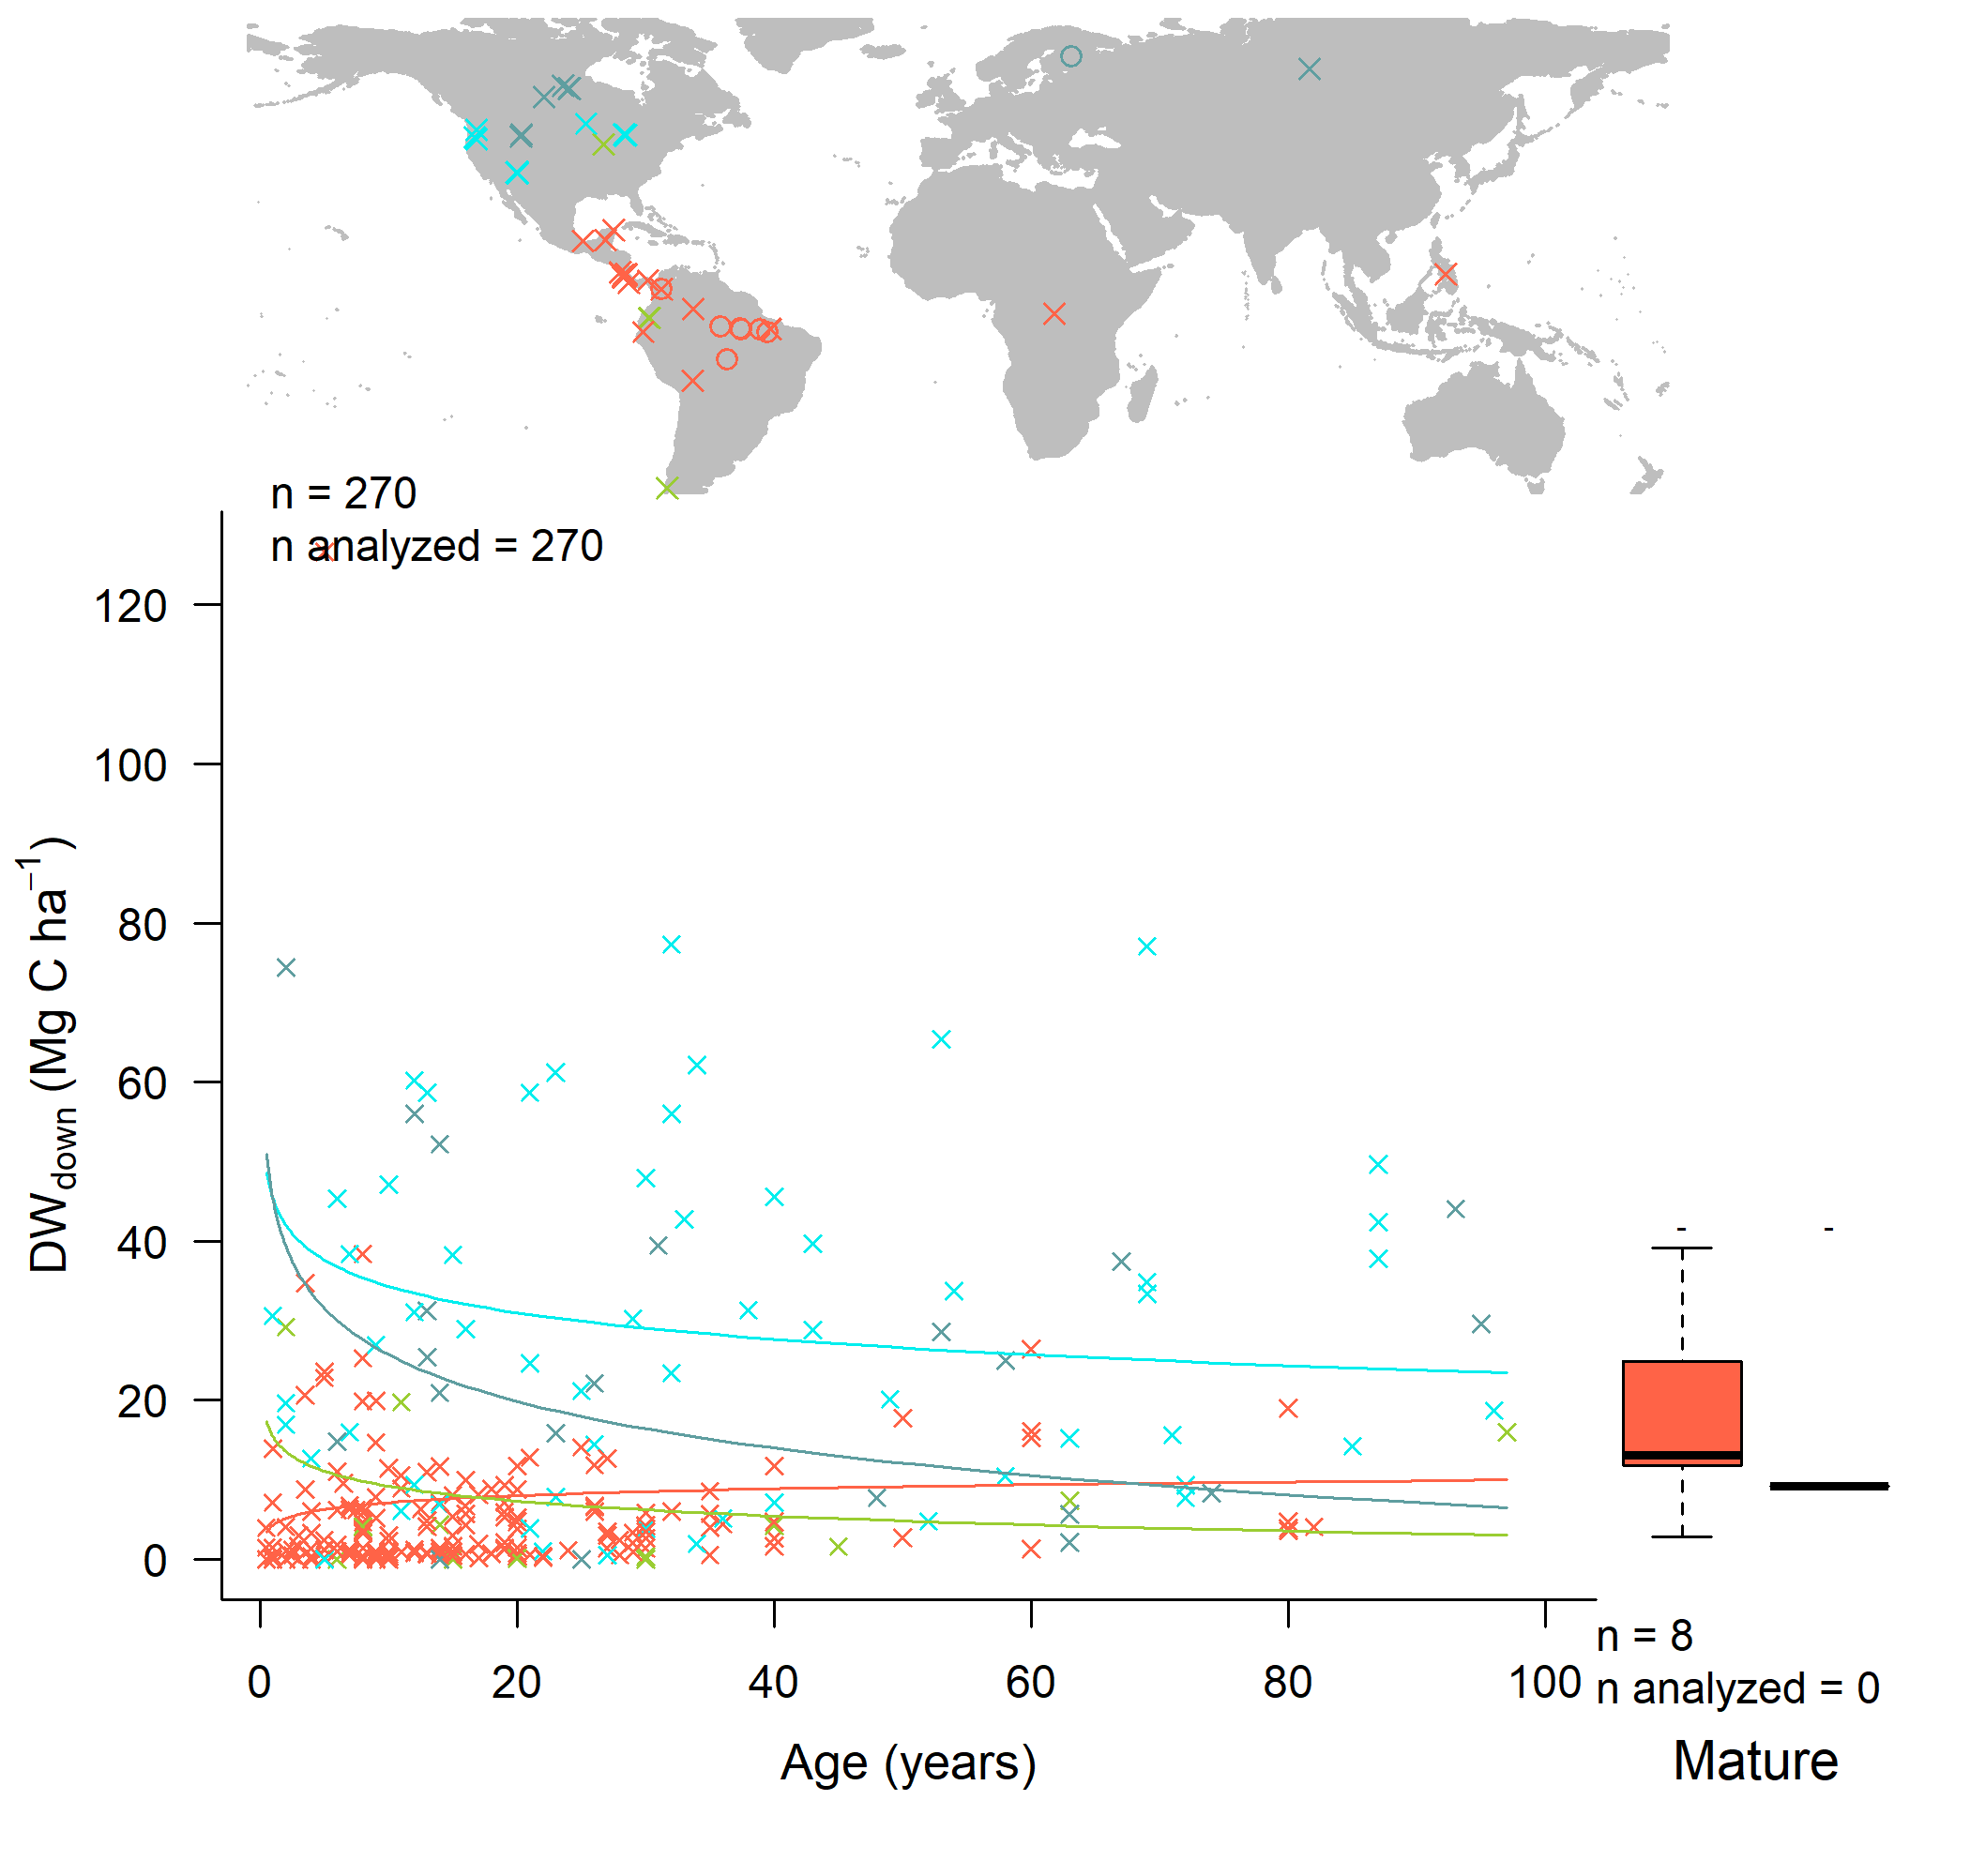
\includegraphics[width=1\linewidth]{tables_figures/age_trends/deadwood_down_with_map} 

}

\caption{Age trends and biome differences for $DW_{down}$. Map shows data sources ('$\times$' and '$\circ$' indicate young and mature stands, respectively). In each panel, the left scatterplot shows age trends in forests up to 100 years old, as characterized by a linear mixed effects model with fixed effects of log10(age) and biome. The fitted line indicates the effect of age (solid lines: significant at p<0.05, dashed lines: non-significant), and non-parallel lines indicate a significant log10(age) $\times$ biome interaction. Boxplot illustrates distribution across mature forests, with different letters indicating significant differences between biomes. Data from biomes that did not meet the sample size criteria (see Methods) are plotted, but lack regression lines (young forests) or test of differences across biomes (mature forests).}\label{fig:unnamed-chunk-32}
\end{figure}

\newpage

\hypertarget{figure-s30.-age-trends-and-biome-differences-for-ol}{%
\subsection{\texorpdfstring{Figure S30. Age trends and biome differences
for
\(OL\)}{Figure S30. Age trends and biome differences for OL}}\label{figure-s30.-age-trends-and-biome-differences-for-ol}}

\begin{figure}[H]

{\centering 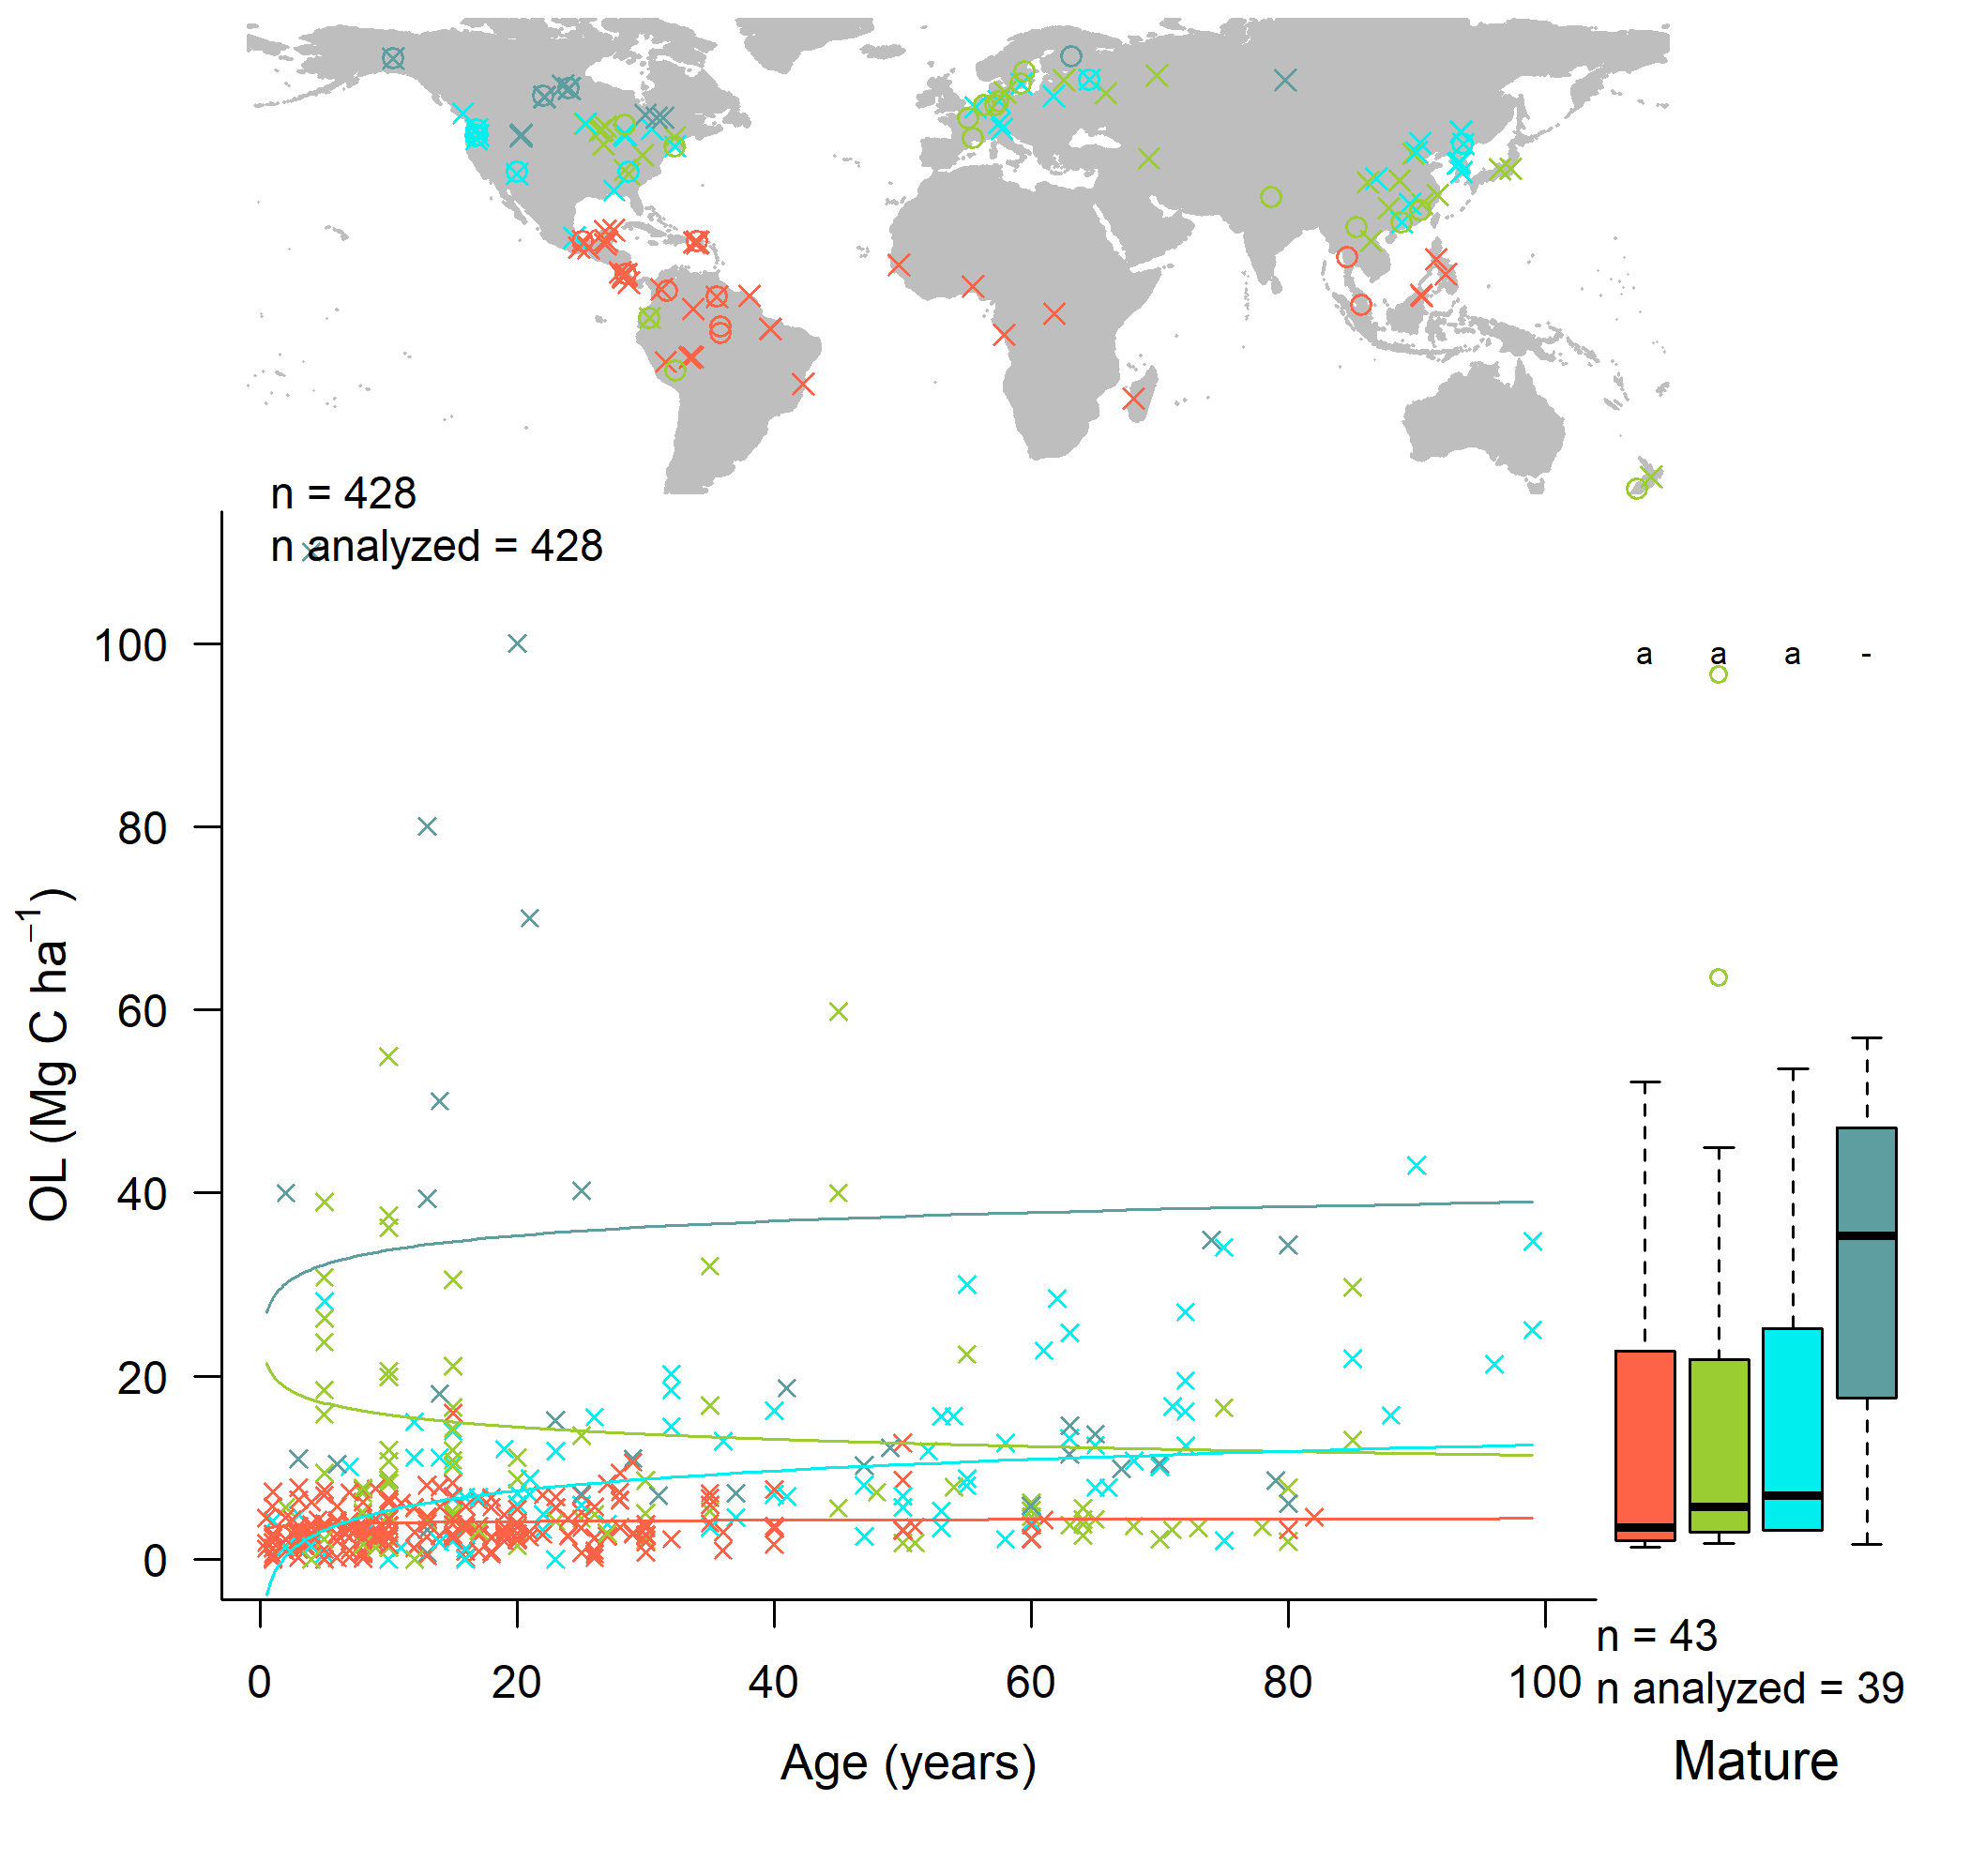
\includegraphics[width=1\linewidth]{tables_figures/age_trends/organic_layer_with_map} 

}

\caption{Age trends and biome differences for $OL$. Map shows data sources ('$\times$' and '$\circ$' indicate young and mature stands, respectively). In each panel, the left scatterplot shows age trends in forests up to 100 years old, as characterized by a linear mixed effects model with fixed effects of log10(age) and biome. The fitted line indicates the effect of age (solid lines: significant at p<0.05, dashed lines: non-significant), and non-parallel lines indicate a significant log10(age) $\times$ biome interaction. Boxplot illustrates distribution across mature forests, with different letters indicating significant differences between biomes. Data from biomes that did not meet the sample size criteria (see Methods) are plotted, but lack regression lines (young forests) or test of differences across biomes (mature forests).}\label{fig:unnamed-chunk-33}
\end{figure}

\end{document}
